\documentclass[twoside]{book}

% Packages required by doxygen
\usepackage{fixltx2e}
\usepackage{calc}
\usepackage{doxygen}
\usepackage[export]{adjustbox} % also loads graphicx
\usepackage{graphicx}
\usepackage[utf8]{inputenc}
\usepackage{makeidx}
\usepackage{multicol}
\usepackage{multirow}
\PassOptionsToPackage{warn}{textcomp}
\usepackage{textcomp}
\usepackage[nointegrals]{wasysym}
\usepackage[table]{xcolor}

% Font selection
\usepackage[T1]{fontenc}
\usepackage[scaled=.90]{helvet}
\usepackage{courier}
\usepackage{amssymb}
\usepackage{sectsty}
\renewcommand{\familydefault}{\sfdefault}
\allsectionsfont{%
  \fontseries{bc}\selectfont%
  \color{darkgray}%
}
\renewcommand{\DoxyLabelFont}{%
  \fontseries{bc}\selectfont%
  \color{darkgray}%
}
\newcommand{\+}{\discretionary{\mbox{\scriptsize$\hookleftarrow$}}{}{}}

% Page & text layout
\usepackage{geometry}
\geometry{%
  a4paper,%
  top=2.5cm,%
  bottom=2.5cm,%
  left=2.5cm,%
  right=2.5cm%
}
\tolerance=750
\hfuzz=15pt
\hbadness=750
\setlength{\emergencystretch}{15pt}
\setlength{\parindent}{0cm}
\setlength{\parskip}{3ex plus 2ex minus 2ex}
\makeatletter
\renewcommand{\paragraph}{%
  \@startsection{paragraph}{4}{0ex}{-1.0ex}{1.0ex}{%
    \normalfont\normalsize\bfseries\SS@parafont%
  }%
}
\renewcommand{\subparagraph}{%
  \@startsection{subparagraph}{5}{0ex}{-1.0ex}{1.0ex}{%
    \normalfont\normalsize\bfseries\SS@subparafont%
  }%
}
\makeatother

% Headers & footers
\usepackage{fancyhdr}
\pagestyle{fancyplain}
\fancyhead[LE]{\fancyplain{}{\bfseries\thepage}}
\fancyhead[CE]{\fancyplain{}{}}
\fancyhead[RE]{\fancyplain{}{\bfseries\leftmark}}
\fancyhead[LO]{\fancyplain{}{\bfseries\rightmark}}
\fancyhead[CO]{\fancyplain{}{}}
\fancyhead[RO]{\fancyplain{}{\bfseries\thepage}}
\fancyfoot[LE]{\fancyplain{}{}}
\fancyfoot[CE]{\fancyplain{}{}}
\fancyfoot[RE]{\fancyplain{}{\bfseries\scriptsize Generated by Doxygen }}
\fancyfoot[LO]{\fancyplain{}{\bfseries\scriptsize Generated by Doxygen }}
\fancyfoot[CO]{\fancyplain{}{}}
\fancyfoot[RO]{\fancyplain{}{}}
\renewcommand{\footrulewidth}{0.4pt}
\renewcommand{\chaptermark}[1]{%
  \markboth{#1}{}%
}
\renewcommand{\sectionmark}[1]{%
  \markright{\thesection\ #1}%
}

% Indices & bibliography
\usepackage{natbib}
\usepackage[titles]{tocloft}
\setcounter{tocdepth}{3}
\setcounter{secnumdepth}{5}
\makeindex

% Hyperlinks (required, but should be loaded last)
\usepackage{ifpdf}
\ifpdf
  \usepackage[pdftex,pagebackref=true]{hyperref}
\else
  \usepackage[ps2pdf,pagebackref=true]{hyperref}
\fi
\hypersetup{%
  colorlinks=true,%
  linkcolor=blue,%
  citecolor=blue,%
  unicode%
}

% Custom commands
\newcommand{\clearemptydoublepage}{%
  \newpage{\pagestyle{empty}\cleardoublepage}%
}

\usepackage{caption}
\captionsetup{labelsep=space,justification=centering,font={bf},singlelinecheck=off,skip=4pt,position=top}

%===== C O N T E N T S =====

\begin{document}

% Titlepage & ToC
\hypersetup{pageanchor=false,
             bookmarksnumbered=true,
             pdfencoding=unicode
            }
\pagenumbering{alph}
\begin{titlepage}
\vspace*{7cm}
\begin{center}%
{\Large Final-\/\+Project-\/\+Group3 }\\
\vspace*{1cm}
{\large Generated by Doxygen 1.8.13}\\
\end{center}
\end{titlepage}
\clearemptydoublepage
\pagenumbering{roman}
\tableofcontents
\clearemptydoublepage
\pagenumbering{arabic}
\hypersetup{pageanchor=true}

%--- Begin generated contents ---
\chapter{Namespace Index}
\section{Namespace List}
Here is a list of all namespaces with brief descriptions\+:\begin{DoxyCompactList}
\item\contentsline{section}{\hyperlink{namespacefp}{fp} }{\pageref{namespacefp}}{}
\end{DoxyCompactList}

\chapter{Hierarchical Index}
\section{Class Hierarchy}
This inheritance list is sorted roughly, but not completely, alphabetically\+:\begin{DoxyCompactList}
\item \contentsline{section}{fp\+:\+:Algorithm}{\pageref{classfp_1_1_algorithm}}{}
\item \contentsline{section}{fp\+:\+:A\+PI}{\pageref{classfp_1_1_a_p_i}}{}
\item \contentsline{section}{fp\+:\+:Land\+Based\+Robot}{\pageref{classfp_1_1_land_based_robot}}{}
\begin{DoxyCompactList}
\item \contentsline{section}{fp\+:\+:Land\+Based\+Tracked}{\pageref{classfp_1_1_land_based_tracked}}{}
\item \contentsline{section}{fp\+:\+:Land\+Based\+Wheeled}{\pageref{classfp_1_1_land_based_wheeled}}{}
\end{DoxyCompactList}
\item \contentsline{section}{fp\+:\+:Maze}{\pageref{classfp_1_1_maze}}{}
\item \contentsline{section}{fp\+:\+:Algorithm\+:\+:Position}{\pageref{structfp_1_1_algorithm_1_1_position}}{}
\end{DoxyCompactList}

\chapter{Class Index}
\section{Class List}
Here are the classes, structs, unions and interfaces with brief descriptions\+:\begin{DoxyCompactList}
\item\contentsline{section}{\hyperlink{classrwa3_1_1_land_based_robot}{rwa3\+::\+Land\+Based\+Robot} }{\pageref{classrwa3_1_1_land_based_robot}}{}
\item\contentsline{section}{\hyperlink{classrwa3_1_1_land_based_tracked}{rwa3\+::\+Land\+Based\+Tracked} }{\pageref{classrwa3_1_1_land_based_tracked}}{}
\item\contentsline{section}{\hyperlink{classrwa3_1_1_land_based_wheeled}{rwa3\+::\+Land\+Based\+Wheeled} }{\pageref{classrwa3_1_1_land_based_wheeled}}{}
\end{DoxyCompactList}

\chapter{File Index}
\section{File List}
Here is a list of all files with brief descriptions\+:\begin{DoxyCompactList}
\item\contentsline{section}{\hyperlink{main_01__backup_8cpp}{main \+\_\+backup.\+cpp} }{\pageref{main_01__backup_8cpp}}{}
\item\contentsline{section}{\hyperlink{main_8cpp}{main.\+cpp} }{\pageref{main_8cpp}}{}
\end{DoxyCompactList}

\chapter{Namespace Documentation}
\hypertarget{namespacefp}{}\section{fp Namespace Reference}
\label{namespacefp}\index{fp@{fp}}
\subsection*{Classes}
\begin{DoxyCompactItemize}
\item 
class \hyperlink{classfp_1_1_algorithm}{Algorithm}
\item 
class \hyperlink{classfp_1_1_a_p_i}{A\+PI}
\item 
class \hyperlink{classfp_1_1_land_based_robot}{Land\+Based\+Robot}
\item 
class \hyperlink{classfp_1_1_land_based_tracked}{Land\+Based\+Tracked}
\item 
class \hyperlink{classfp_1_1_land_based_wheeled}{Land\+Based\+Wheeled}
\item 
class \hyperlink{classfp_1_1_maze}{Maze}
\end{DoxyCompactItemize}


\subsection{Detailed Description}
\hyperlink{_maze_8h}{Maze.\+h}

$<$ \hyperlink{landbasedwheeled_8h}{Land\+Based\+Wheeled.\+h} , Derived concrete class

$<$ \hyperlink{_land_based_robot_8h}{Land\+Based\+Robot.\+h} , Base abstract class

Header for \hyperlink{classfp_1_1_a_p_i}{A\+PI} Class Scenario\+: A robot navigates through a maze to reach the center of the maze. This project uses an open source simulator (\href{https://github.com/mackorone/mms}{\tt https\+://github.\+com/mackorone/mms}) to visualize path planning algorithms. The interaction between this program and the simulator can be performed using built-\/in methods from the \hyperlink{classfp_1_1_a_p_i}{A\+PI} class. These methods can be found at \href{https://github.com/mackorone/mms}{\tt https\+://github.\+com/mackorone/mms} and have been implemented in the function definitions below.

\hyperlink{_algorithm_8h}{Algorithm.\+h} 
\chapter{Class Documentation}
\hypertarget{classfp_1_1_algorithm}{}\section{fp\+:\+:Algorithm Class Reference}
\label{classfp_1_1_algorithm}\index{fp\+::\+Algorithm@{fp\+::\+Algorithm}}


{\ttfamily \#include $<$Algorithm.\+h$>$}



Collaboration diagram for fp\+:\+:Algorithm\+:\nopagebreak
\begin{figure}[H]
\begin{center}
\leavevmode
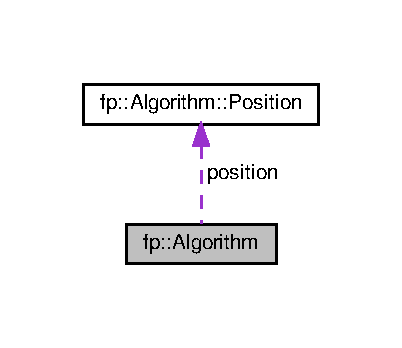
\includegraphics[width=266pt]{classfp_1_1_algorithm__coll__graph}
\end{center}
\end{figure}
\subsection*{Classes}
\begin{DoxyCompactItemize}
\item 
struct \hyperlink{structfp_1_1_algorithm_1_1_position}{Position}
\end{DoxyCompactItemize}
\subsection*{Public Member Functions}
\begin{DoxyCompactItemize}
\item 
void \hyperlink{classfp_1_1_algorithm_ab91291b423ce58ba86e317112ca0c5ba}{Update\+Direction} (char \&current\+\_\+direction, char turn)
\item 
void \hyperlink{classfp_1_1_algorithm_a14f37fd87d690a5db6a38ea63cd1aeb1}{Update\+Position} (char current\+\_\+direction, char move, std\+::array$<$ int, 2 $>$ \&\hyperlink{classfp_1_1_algorithm_a88395e8c0b52c4aef33b41caff21300c}{curr\+\_\+node})
\item 
void \hyperlink{classfp_1_1_algorithm_ac6e4cae1f140d0155f2feaaaf1d287c1}{Solve} ()
\item 
void \hyperlink{classfp_1_1_algorithm_a5c0c5a23c677797bbe4b9616f1bfded6}{D\+FS} (bool start, char current\+\_\+direction, const std\+::shared\+\_\+ptr$<$ \hyperlink{classfp_1_1_land_based_robot}{fp\+::\+Land\+Based\+Robot} $>$ \&robot)
\item 
bool \hyperlink{classfp_1_1_algorithm_a169e9e4e400a85687aa6554a3cbd2e04}{Reset\+Pressed} ()
\item 
void \hyperlink{classfp_1_1_algorithm_a182de09af3489ef37ea0fd4a4baeacbc}{reset} ()
\item 
void \hyperlink{classfp_1_1_algorithm_a434cfecd6898f4e89ba632433fa19afd}{Call\+Set\+Maze} ()
\item 
void \hyperlink{classfp_1_1_algorithm_ac82185822a00aa4b08266207ca4b7e26}{Check\+Wall} (std\+::array$<$ int, 2 $>$ \hyperlink{classfp_1_1_algorithm_a88395e8c0b52c4aef33b41caff21300c}{curr\+\_\+node}, char \&current\+\_\+direction, std\+::array$<$ std\+::array$<$ bool, 16 $>$, 16 $>$ \hyperlink{classfp_1_1_algorithm_a41904cf962dd8c46901d39ab03d77545}{visited\+\_\+node\+\_\+})
\item 
void \hyperlink{classfp_1_1_algorithm_a363e9198e1a2f95caa581b5b9e90efb6}{Find\+Next\+Node} (std\+::array$<$ int, 2 $>$ \hyperlink{classfp_1_1_algorithm_a88395e8c0b52c4aef33b41caff21300c}{curr\+\_\+node}, char \&current\+\_\+direction, bool \hyperlink{classfp_1_1_algorithm_a7a37ba8431c685c42f305a73812efecb}{path\+\_\+blocked\+\_\+})
\item 
bool \hyperlink{classfp_1_1_algorithm_a2309270f8f6276d6f421328239269d3a}{Check\+Dead\+End} (std\+::array$<$ int, 2 $>$ \hyperlink{classfp_1_1_algorithm_a88395e8c0b52c4aef33b41caff21300c}{curr\+\_\+node}, char current\+\_\+direction)
\item 
void \hyperlink{classfp_1_1_algorithm_ab272faa6f88e5edbe2f8c19b2988ae16}{Back\+Track} (std\+::array$<$ int, 2 $>$ \hyperlink{classfp_1_1_algorithm_a88395e8c0b52c4aef33b41caff21300c}{curr\+\_\+node}, char \&current\+\_\+direction, std\+::array$<$ std\+::array$<$ bool, 16 $>$, 16 $>$ \&\hyperlink{classfp_1_1_algorithm_a41904cf962dd8c46901d39ab03d77545}{visited\+\_\+node\+\_\+})
\item 
bool \hyperlink{classfp_1_1_algorithm_a9270347a0ca5be0f7717e6772de5f87c}{Check\+Path} (std\+::array$<$ int, 2 $>$ \hyperlink{classfp_1_1_algorithm_ac3672498d86469ee445fe66a140952cb}{next\+\_\+node}, std\+::array$<$ std\+::array$<$ bool, 16 $>$, 16 $>$ \hyperlink{classfp_1_1_algorithm_a41904cf962dd8c46901d39ab03d77545}{visited\+\_\+node\+\_\+})
\item 
\hyperlink{classfp_1_1_algorithm_adaa1af41614b0d95c2a940cc87c68a2e}{Algorithm} ()
\item 
\hyperlink{classfp_1_1_algorithm_aefb8012b9e6457191d7fc16affe5a700}{$\sim$\+Algorithm} ()=default
\end{DoxyCompactItemize}
\subsection*{Static Public Member Functions}
\begin{DoxyCompactItemize}
\item 
static void \hyperlink{classfp_1_1_algorithm_ad8d891300bf2a5be160a629a93e7058d}{log} (const std\+::string \&text)
\item 
static void \hyperlink{classfp_1_1_algorithm_a69fe7bd633b0e23593e7808babe4e90d}{Initialize\+Maze} (\hyperlink{structfp_1_1_algorithm_1_1_position}{fp\+::\+Algorithm\+::\+Position} \&\hyperlink{classfp_1_1_algorithm_a841339b57c3d2739325f3f421ada43b6}{position}, char \&\hyperlink{classfp_1_1_algorithm_afdbf632b658aea1aef75caa90e60a8fc}{direction})
\end{DoxyCompactItemize}
\subsection*{Public Attributes}
\begin{DoxyCompactItemize}
\item 
struct \hyperlink{structfp_1_1_algorithm_1_1_position}{fp\+::\+Algorithm\+::\+Position} \hyperlink{classfp_1_1_algorithm_a841339b57c3d2739325f3f421ada43b6}{position}
\item 
struct \hyperlink{structfp_1_1_algorithm_1_1_position}{fp\+::\+Algorithm\+::\+Position} \hyperlink{classfp_1_1_algorithm_a94d3b3797f19988f49fbda76013c3899}{current\+\_\+pos}
\item 
std\+::stack$<$ std\+::array$<$ int, 2 $>$ $>$ \hyperlink{classfp_1_1_algorithm_a3a646d05e1d457e73608134417b55113}{stack\+\_\+}
\item 
std\+::shared\+\_\+ptr$<$ \hyperlink{classfp_1_1_land_based_robot}{fp\+::\+Land\+Based\+Robot} $>$ \hyperlink{classfp_1_1_algorithm_a9937e133d060b6216a30055dc400ac10}{robot\+\_\+}
\end{DoxyCompactItemize}
\subsection*{Protected Member Functions}
\begin{DoxyCompactItemize}
\item 
void \hyperlink{classfp_1_1_algorithm_ac289d75b6850d5ad4a888360b3cfeda9}{Clear\+Stack} ()
\end{DoxyCompactItemize}
\subsection*{Protected Attributes}
\begin{DoxyCompactItemize}
\item 
\hyperlink{classfp_1_1_maze}{Maze} \hyperlink{classfp_1_1_algorithm_a5eaa9074986ebf65f2f549f78eedd0f2}{maze}
\item 
char \hyperlink{classfp_1_1_algorithm_afdbf632b658aea1aef75caa90e60a8fc}{direction} \{\textquotesingle{}n\textquotesingle{}\}
\item 
std\+::array$<$ std\+::array$<$ bool, 16 $>$, 16 $>$ \hyperlink{classfp_1_1_algorithm_a41904cf962dd8c46901d39ab03d77545}{visited\+\_\+node\+\_\+} \{false\}
\item 
std\+::array$<$ int, 2 $>$ \hyperlink{classfp_1_1_algorithm_a88395e8c0b52c4aef33b41caff21300c}{curr\+\_\+node} = \{0, 0\}
\item 
std\+::array$<$ int, 2 $>$ \hyperlink{classfp_1_1_algorithm_ac3672498d86469ee445fe66a140952cb}{next\+\_\+node}
\item 
std\+::array$<$ int, 2 $>$ \hyperlink{classfp_1_1_algorithm_ac90048223f33b81908e9c7367ec355bc}{parent\+\_\+node}
\item 
std\+::array$<$ int, 2 $>$ \hyperlink{classfp_1_1_algorithm_a9fcc4bf2df720fef33da5705cd317480}{goal\+\_\+1}
\item 
std\+::array$<$ int, 2 $>$ \hyperlink{classfp_1_1_algorithm_aa01beb678f2db28d33e32f1060341bcc}{goal\+\_\+2}
\item 
std\+::array$<$ int, 2 $>$ \hyperlink{classfp_1_1_algorithm_a8e8b41783484c3a30ae85bcd978d5e46}{goal\+\_\+3}
\item 
std\+::array$<$ int, 2 $>$ \hyperlink{classfp_1_1_algorithm_a9832306da6877eba455ef5160c4a7f86}{goal\+\_\+4}
\item 
bool \hyperlink{classfp_1_1_algorithm_a7a37ba8431c685c42f305a73812efecb}{path\+\_\+blocked\+\_\+} \{true\}
\end{DoxyCompactItemize}


\subsection{Constructor \& Destructor Documentation}
\mbox{\Hypertarget{classfp_1_1_algorithm_adaa1af41614b0d95c2a940cc87c68a2e}\label{classfp_1_1_algorithm_adaa1af41614b0d95c2a940cc87c68a2e}} 
\index{fp\+::\+Algorithm@{fp\+::\+Algorithm}!Algorithm@{Algorithm}}
\index{Algorithm@{Algorithm}!fp\+::\+Algorithm@{fp\+::\+Algorithm}}
\subsubsection{\texorpdfstring{Algorithm()}{Algorithm()}}
{\footnotesize\ttfamily fp\+::\+Algorithm\+::\+Algorithm (\begin{DoxyParamCaption}{ }\end{DoxyParamCaption})\hspace{0.3cm}{\ttfamily [inline]}}

\mbox{\Hypertarget{classfp_1_1_algorithm_aefb8012b9e6457191d7fc16affe5a700}\label{classfp_1_1_algorithm_aefb8012b9e6457191d7fc16affe5a700}} 
\index{fp\+::\+Algorithm@{fp\+::\+Algorithm}!````~Algorithm@{$\sim$\+Algorithm}}
\index{````~Algorithm@{$\sim$\+Algorithm}!fp\+::\+Algorithm@{fp\+::\+Algorithm}}
\subsubsection{\texorpdfstring{$\sim$\+Algorithm()}{~Algorithm()}}
{\footnotesize\ttfamily fp\+::\+Algorithm\+::$\sim$\+Algorithm (\begin{DoxyParamCaption}{ }\end{DoxyParamCaption})\hspace{0.3cm}{\ttfamily [default]}}



\subsection{Member Function Documentation}
\mbox{\Hypertarget{classfp_1_1_algorithm_ab272faa6f88e5edbe2f8c19b2988ae16}\label{classfp_1_1_algorithm_ab272faa6f88e5edbe2f8c19b2988ae16}} 
\index{fp\+::\+Algorithm@{fp\+::\+Algorithm}!Back\+Track@{Back\+Track}}
\index{Back\+Track@{Back\+Track}!fp\+::\+Algorithm@{fp\+::\+Algorithm}}
\subsubsection{\texorpdfstring{Back\+Track()}{BackTrack()}}
{\footnotesize\ttfamily void fp\+::\+Algorithm\+::\+Back\+Track (\begin{DoxyParamCaption}\item[{std\+::array$<$ int, 2 $>$}]{curr\+\_\+node,  }\item[{char \&}]{current\+\_\+direction,  }\item[{std\+::array$<$ std\+::array$<$ bool, 16 $>$, 16 $>$ \&}]{visited\+\_\+node\+\_\+ }\end{DoxyParamCaption})}


\begin{DoxyParams}{Parameters}
{\em curr\+\_\+node} & \\
\hline
{\em visited\+\_\+node\+\_\+} & \\
\hline
\end{DoxyParams}
\mbox{\Hypertarget{classfp_1_1_algorithm_a434cfecd6898f4e89ba632433fa19afd}\label{classfp_1_1_algorithm_a434cfecd6898f4e89ba632433fa19afd}} 
\index{fp\+::\+Algorithm@{fp\+::\+Algorithm}!Call\+Set\+Maze@{Call\+Set\+Maze}}
\index{Call\+Set\+Maze@{Call\+Set\+Maze}!fp\+::\+Algorithm@{fp\+::\+Algorithm}}
\subsubsection{\texorpdfstring{Call\+Set\+Maze()}{CallSetMaze()}}
{\footnotesize\ttfamily void fp\+::\+Algorithm\+::\+Call\+Set\+Maze (\begin{DoxyParamCaption}{ }\end{DoxyParamCaption})}

Function to set the center and perimeter of the maze \mbox{\Hypertarget{classfp_1_1_algorithm_a2309270f8f6276d6f421328239269d3a}\label{classfp_1_1_algorithm_a2309270f8f6276d6f421328239269d3a}} 
\index{fp\+::\+Algorithm@{fp\+::\+Algorithm}!Check\+Dead\+End@{Check\+Dead\+End}}
\index{Check\+Dead\+End@{Check\+Dead\+End}!fp\+::\+Algorithm@{fp\+::\+Algorithm}}
\subsubsection{\texorpdfstring{Check\+Dead\+End()}{CheckDeadEnd()}}
{\footnotesize\ttfamily bool fp\+::\+Algorithm\+::\+Check\+Dead\+End (\begin{DoxyParamCaption}\item[{std\+::array$<$ int, 2 $>$}]{curr\+\_\+node,  }\item[{char}]{current\+\_\+direction }\end{DoxyParamCaption})}

\mbox{\Hypertarget{classfp_1_1_algorithm_a9270347a0ca5be0f7717e6772de5f87c}\label{classfp_1_1_algorithm_a9270347a0ca5be0f7717e6772de5f87c}} 
\index{fp\+::\+Algorithm@{fp\+::\+Algorithm}!Check\+Path@{Check\+Path}}
\index{Check\+Path@{Check\+Path}!fp\+::\+Algorithm@{fp\+::\+Algorithm}}
\subsubsection{\texorpdfstring{Check\+Path()}{CheckPath()}}
{\footnotesize\ttfamily bool fp\+::\+Algorithm\+::\+Check\+Path (\begin{DoxyParamCaption}\item[{std\+::array$<$ int, 2 $>$}]{next\+\_\+node,  }\item[{std\+::array$<$ std\+::array$<$ bool, 16 $>$, 16 $>$}]{visited\+\_\+node\+\_\+ }\end{DoxyParamCaption})}

Check\+Path function sees if the next node has been visited or a wall 
\begin{DoxyParams}{Parameters}
{\em path\+\_\+blocked\+\_\+} & boolean to see if path is blocked by a wall \\
\hline
{\em next\+\_\+node} & next node array in terms of position \\
\hline
{\em visited\+\_\+node\+\_\+} & 16x16 boolean array to determine if a node has been visited \\
\hline
\end{DoxyParams}
\begin{DoxyReturn}{Returns}
true or false if path can be moved to 
\end{DoxyReturn}
\mbox{\Hypertarget{classfp_1_1_algorithm_ac82185822a00aa4b08266207ca4b7e26}\label{classfp_1_1_algorithm_ac82185822a00aa4b08266207ca4b7e26}} 
\index{fp\+::\+Algorithm@{fp\+::\+Algorithm}!Check\+Wall@{Check\+Wall}}
\index{Check\+Wall@{Check\+Wall}!fp\+::\+Algorithm@{fp\+::\+Algorithm}}
\subsubsection{\texorpdfstring{Check\+Wall()}{CheckWall()}}
{\footnotesize\ttfamily void fp\+::\+Algorithm\+::\+Check\+Wall (\begin{DoxyParamCaption}\item[{std\+::array$<$ int, 2 $>$}]{curr\+\_\+node,  }\item[{char \&}]{current\+\_\+direction,  }\item[{std\+::array$<$ std\+::array$<$ bool, 16 $>$, 16 $>$}]{visited\+\_\+node\+\_\+ }\end{DoxyParamCaption})}

Check\+Wall is a method to check if there is a wall in the front, left, and right side of the robot 
\begin{DoxyParams}{Parameters}
{\em current\+\_\+position} & current position of the robot \\
\hline
{\em direction} & direction that the robot is facing \\
\hline
\end{DoxyParams}
\begin{DoxyReturn}{Returns}

\end{DoxyReturn}
\mbox{\Hypertarget{classfp_1_1_algorithm_ac289d75b6850d5ad4a888360b3cfeda9}\label{classfp_1_1_algorithm_ac289d75b6850d5ad4a888360b3cfeda9}} 
\index{fp\+::\+Algorithm@{fp\+::\+Algorithm}!Clear\+Stack@{Clear\+Stack}}
\index{Clear\+Stack@{Clear\+Stack}!fp\+::\+Algorithm@{fp\+::\+Algorithm}}
\subsubsection{\texorpdfstring{Clear\+Stack()}{ClearStack()}}
{\footnotesize\ttfamily void fp\+::\+Algorithm\+::\+Clear\+Stack (\begin{DoxyParamCaption}{ }\end{DoxyParamCaption})\hspace{0.3cm}{\ttfamily [protected]}}

\mbox{\Hypertarget{classfp_1_1_algorithm_a5c0c5a23c677797bbe4b9616f1bfded6}\label{classfp_1_1_algorithm_a5c0c5a23c677797bbe4b9616f1bfded6}} 
\index{fp\+::\+Algorithm@{fp\+::\+Algorithm}!D\+FS@{D\+FS}}
\index{D\+FS@{D\+FS}!fp\+::\+Algorithm@{fp\+::\+Algorithm}}
\subsubsection{\texorpdfstring{D\+F\+S()}{DFS()}}
{\footnotesize\ttfamily void fp\+::\+Algorithm\+::\+D\+FS (\begin{DoxyParamCaption}\item[{bool}]{start,  }\item[{char}]{current\+\_\+direction,  }\item[{const std\+::shared\+\_\+ptr$<$ \hyperlink{classfp_1_1_land_based_robot}{fp\+::\+Land\+Based\+Robot} $>$ \&}]{robot }\end{DoxyParamCaption})}

Depth First Search \hyperlink{classfp_1_1_algorithm}{Algorithm} to traverse through the maze and save visited nodes, starts with checking south then east, north, and west, in counterclockwise order 
\begin{DoxyParams}{Parameters}
{\em start} & tells the algorithm if first time starting it \\
\hline
{\em current\+\_\+direction} & current direction of the robot \\
\hline
{\em robot} & pointer to one of the available robots, wheeled/tracked \\
\hline
\end{DoxyParams}
\mbox{\Hypertarget{classfp_1_1_algorithm_a363e9198e1a2f95caa581b5b9e90efb6}\label{classfp_1_1_algorithm_a363e9198e1a2f95caa581b5b9e90efb6}} 
\index{fp\+::\+Algorithm@{fp\+::\+Algorithm}!Find\+Next\+Node@{Find\+Next\+Node}}
\index{Find\+Next\+Node@{Find\+Next\+Node}!fp\+::\+Algorithm@{fp\+::\+Algorithm}}
\subsubsection{\texorpdfstring{Find\+Next\+Node()}{FindNextNode()}}
{\footnotesize\ttfamily void fp\+::\+Algorithm\+::\+Find\+Next\+Node (\begin{DoxyParamCaption}\item[{std\+::array$<$ int, 2 $>$}]{curr\+\_\+node,  }\item[{char \&}]{current\+\_\+direction,  }\item[{bool}]{path\+\_\+blocked\+\_\+ }\end{DoxyParamCaption})}

Find\+Next\+Node function checks 1 node forward in every direction and sees if the path is blocked or is visited to determine which direction the robot can go to 
\begin{DoxyParams}{Parameters}
{\em curr\+\_\+node} & current node array, for x and y position \\
\hline
{\em current\+\_\+direction} & current direction of the robot \\
\hline
{\em path\+\_\+blocked\+\_\+} & boolean to see if the path is blocked \\
\hline
\end{DoxyParams}
Arrays to define the possible direction of the nodes , north, south, east, west\mbox{\Hypertarget{classfp_1_1_algorithm_a69fe7bd633b0e23593e7808babe4e90d}\label{classfp_1_1_algorithm_a69fe7bd633b0e23593e7808babe4e90d}} 
\index{fp\+::\+Algorithm@{fp\+::\+Algorithm}!Initialize\+Maze@{Initialize\+Maze}}
\index{Initialize\+Maze@{Initialize\+Maze}!fp\+::\+Algorithm@{fp\+::\+Algorithm}}
\subsubsection{\texorpdfstring{Initialize\+Maze()}{InitializeMaze()}}
{\footnotesize\ttfamily void fp\+::\+Algorithm\+::\+Initialize\+Maze (\begin{DoxyParamCaption}\item[{\hyperlink{structfp_1_1_algorithm_1_1_position}{fp\+::\+Algorithm\+::\+Position} \&}]{position,  }\item[{char \&}]{direction }\end{DoxyParamCaption})\hspace{0.3cm}{\ttfamily [static]}}

Initializes the maze with default settings 
\begin{DoxyParams}{Parameters}
{\em position} & structure for x y coordinates, sets to 0 for initialization \\
\hline
{\em direction} & character to assign the robot direction n, s, e, w \\
\hline
\end{DoxyParams}
\mbox{\Hypertarget{classfp_1_1_algorithm_ad8d891300bf2a5be160a629a93e7058d}\label{classfp_1_1_algorithm_ad8d891300bf2a5be160a629a93e7058d}} 
\index{fp\+::\+Algorithm@{fp\+::\+Algorithm}!log@{log}}
\index{log@{log}!fp\+::\+Algorithm@{fp\+::\+Algorithm}}
\subsubsection{\texorpdfstring{log()}{log()}}
{\footnotesize\ttfamily void fp\+::\+Algorithm\+::log (\begin{DoxyParamCaption}\item[{const std\+::string \&}]{text }\end{DoxyParamCaption})\hspace{0.3cm}{\ttfamily [static]}}

A method to print out text to the maze simulator 
\begin{DoxyParams}{Parameters}
{\em text} & Message\\
\hline
\end{DoxyParams}
\hyperlink{_algorithm_8cpp}{Algorithm.\+cpp} \mbox{\Hypertarget{classfp_1_1_algorithm_a182de09af3489ef37ea0fd4a4baeacbc}\label{classfp_1_1_algorithm_a182de09af3489ef37ea0fd4a4baeacbc}} 
\index{fp\+::\+Algorithm@{fp\+::\+Algorithm}!reset@{reset}}
\index{reset@{reset}!fp\+::\+Algorithm@{fp\+::\+Algorithm}}
\subsubsection{\texorpdfstring{reset()}{reset()}}
{\footnotesize\ttfamily void fp\+::\+Algorithm\+::reset (\begin{DoxyParamCaption}{ }\end{DoxyParamCaption})}

Resets the maze if the button is pressed \mbox{\Hypertarget{classfp_1_1_algorithm_a169e9e4e400a85687aa6554a3cbd2e04}\label{classfp_1_1_algorithm_a169e9e4e400a85687aa6554a3cbd2e04}} 
\index{fp\+::\+Algorithm@{fp\+::\+Algorithm}!Reset\+Pressed@{Reset\+Pressed}}
\index{Reset\+Pressed@{Reset\+Pressed}!fp\+::\+Algorithm@{fp\+::\+Algorithm}}
\subsubsection{\texorpdfstring{Reset\+Pressed()}{ResetPressed()}}
{\footnotesize\ttfamily bool fp\+::\+Algorithm\+::\+Reset\+Pressed (\begin{DoxyParamCaption}{ }\end{DoxyParamCaption})}

If the reset button is pressed \begin{DoxyReturn}{Returns}
reset 
\end{DoxyReturn}
\mbox{\Hypertarget{classfp_1_1_algorithm_ac6e4cae1f140d0155f2feaaaf1d287c1}\label{classfp_1_1_algorithm_ac6e4cae1f140d0155f2feaaaf1d287c1}} 
\index{fp\+::\+Algorithm@{fp\+::\+Algorithm}!Solve@{Solve}}
\index{Solve@{Solve}!fp\+::\+Algorithm@{fp\+::\+Algorithm}}
\subsubsection{\texorpdfstring{Solve()}{Solve()}}
{\footnotesize\ttfamily void fp\+::\+Algorithm\+::\+Solve (\begin{DoxyParamCaption}{ }\end{DoxyParamCaption})}

Starts the setup for the maze and algorithm \mbox{\Hypertarget{classfp_1_1_algorithm_ab91291b423ce58ba86e317112ca0c5ba}\label{classfp_1_1_algorithm_ab91291b423ce58ba86e317112ca0c5ba}} 
\index{fp\+::\+Algorithm@{fp\+::\+Algorithm}!Update\+Direction@{Update\+Direction}}
\index{Update\+Direction@{Update\+Direction}!fp\+::\+Algorithm@{fp\+::\+Algorithm}}
\subsubsection{\texorpdfstring{Update\+Direction()}{UpdateDirection()}}
{\footnotesize\ttfamily void fp\+::\+Algorithm\+::\+Update\+Direction (\begin{DoxyParamCaption}\item[{char \&}]{current\+\_\+direction,  }\item[{char}]{turn }\end{DoxyParamCaption})}

Function to update the direction of the robot 
\begin{DoxyParams}{Parameters}
{\em current\+\_\+direction} & char direction of N/\+S/\+E/W \\
\hline
{\em turn} & char to specify if the robot is turning left or right \\
\hline
\end{DoxyParams}
\mbox{\Hypertarget{classfp_1_1_algorithm_a14f37fd87d690a5db6a38ea63cd1aeb1}\label{classfp_1_1_algorithm_a14f37fd87d690a5db6a38ea63cd1aeb1}} 
\index{fp\+::\+Algorithm@{fp\+::\+Algorithm}!Update\+Position@{Update\+Position}}
\index{Update\+Position@{Update\+Position}!fp\+::\+Algorithm@{fp\+::\+Algorithm}}
\subsubsection{\texorpdfstring{Update\+Position()}{UpdatePosition()}}
{\footnotesize\ttfamily void fp\+::\+Algorithm\+::\+Update\+Position (\begin{DoxyParamCaption}\item[{char}]{current\+\_\+direction,  }\item[{char}]{move,  }\item[{std\+::array$<$ int, 2 $>$ \&}]{curr\+\_\+node }\end{DoxyParamCaption})}

Function to update the position of the robot 
\begin{DoxyParams}{Parameters}
{\em current\+\_\+direction} & char direction of N/\+S/\+E/W \\
\hline
{\em move} & character to define if the robot moved forward \\
\hline
{\em curr\+\_\+pos} & array to specify current node/cell of robot \\
\hline
\end{DoxyParams}


\subsection{Member Data Documentation}
\mbox{\Hypertarget{classfp_1_1_algorithm_a88395e8c0b52c4aef33b41caff21300c}\label{classfp_1_1_algorithm_a88395e8c0b52c4aef33b41caff21300c}} 
\index{fp\+::\+Algorithm@{fp\+::\+Algorithm}!curr\+\_\+node@{curr\+\_\+node}}
\index{curr\+\_\+node@{curr\+\_\+node}!fp\+::\+Algorithm@{fp\+::\+Algorithm}}
\subsubsection{\texorpdfstring{curr\+\_\+node}{curr\_node}}
{\footnotesize\ttfamily std\+::array$<$int, 2$>$ fp\+::\+Algorithm\+::curr\+\_\+node = \{0, 0\}\hspace{0.3cm}{\ttfamily [protected]}}

\mbox{\Hypertarget{classfp_1_1_algorithm_a94d3b3797f19988f49fbda76013c3899}\label{classfp_1_1_algorithm_a94d3b3797f19988f49fbda76013c3899}} 
\index{fp\+::\+Algorithm@{fp\+::\+Algorithm}!current\+\_\+pos@{current\+\_\+pos}}
\index{current\+\_\+pos@{current\+\_\+pos}!fp\+::\+Algorithm@{fp\+::\+Algorithm}}
\subsubsection{\texorpdfstring{current\+\_\+pos}{current\_pos}}
{\footnotesize\ttfamily struct \hyperlink{structfp_1_1_algorithm_1_1_position}{fp\+::\+Algorithm\+::\+Position}  fp\+::\+Algorithm\+::current\+\_\+pos}

\mbox{\Hypertarget{classfp_1_1_algorithm_afdbf632b658aea1aef75caa90e60a8fc}\label{classfp_1_1_algorithm_afdbf632b658aea1aef75caa90e60a8fc}} 
\index{fp\+::\+Algorithm@{fp\+::\+Algorithm}!direction@{direction}}
\index{direction@{direction}!fp\+::\+Algorithm@{fp\+::\+Algorithm}}
\subsubsection{\texorpdfstring{direction}{direction}}
{\footnotesize\ttfamily char fp\+::\+Algorithm\+::direction \{\textquotesingle{}n\textquotesingle{}\}\hspace{0.3cm}{\ttfamily [protected]}}

\mbox{\Hypertarget{classfp_1_1_algorithm_a9fcc4bf2df720fef33da5705cd317480}\label{classfp_1_1_algorithm_a9fcc4bf2df720fef33da5705cd317480}} 
\index{fp\+::\+Algorithm@{fp\+::\+Algorithm}!goal\+\_\+1@{goal\+\_\+1}}
\index{goal\+\_\+1@{goal\+\_\+1}!fp\+::\+Algorithm@{fp\+::\+Algorithm}}
\subsubsection{\texorpdfstring{goal\+\_\+1}{goal\_1}}
{\footnotesize\ttfamily std\+::array$<$int, 2$>$ fp\+::\+Algorithm\+::goal\+\_\+1\hspace{0.3cm}{\ttfamily [protected]}}

\mbox{\Hypertarget{classfp_1_1_algorithm_aa01beb678f2db28d33e32f1060341bcc}\label{classfp_1_1_algorithm_aa01beb678f2db28d33e32f1060341bcc}} 
\index{fp\+::\+Algorithm@{fp\+::\+Algorithm}!goal\+\_\+2@{goal\+\_\+2}}
\index{goal\+\_\+2@{goal\+\_\+2}!fp\+::\+Algorithm@{fp\+::\+Algorithm}}
\subsubsection{\texorpdfstring{goal\+\_\+2}{goal\_2}}
{\footnotesize\ttfamily std\+::array$<$int, 2$>$ fp\+::\+Algorithm\+::goal\+\_\+2\hspace{0.3cm}{\ttfamily [protected]}}

\mbox{\Hypertarget{classfp_1_1_algorithm_a8e8b41783484c3a30ae85bcd978d5e46}\label{classfp_1_1_algorithm_a8e8b41783484c3a30ae85bcd978d5e46}} 
\index{fp\+::\+Algorithm@{fp\+::\+Algorithm}!goal\+\_\+3@{goal\+\_\+3}}
\index{goal\+\_\+3@{goal\+\_\+3}!fp\+::\+Algorithm@{fp\+::\+Algorithm}}
\subsubsection{\texorpdfstring{goal\+\_\+3}{goal\_3}}
{\footnotesize\ttfamily std\+::array$<$int, 2$>$ fp\+::\+Algorithm\+::goal\+\_\+3\hspace{0.3cm}{\ttfamily [protected]}}

\mbox{\Hypertarget{classfp_1_1_algorithm_a9832306da6877eba455ef5160c4a7f86}\label{classfp_1_1_algorithm_a9832306da6877eba455ef5160c4a7f86}} 
\index{fp\+::\+Algorithm@{fp\+::\+Algorithm}!goal\+\_\+4@{goal\+\_\+4}}
\index{goal\+\_\+4@{goal\+\_\+4}!fp\+::\+Algorithm@{fp\+::\+Algorithm}}
\subsubsection{\texorpdfstring{goal\+\_\+4}{goal\_4}}
{\footnotesize\ttfamily std\+::array$<$int, 2$>$ fp\+::\+Algorithm\+::goal\+\_\+4\hspace{0.3cm}{\ttfamily [protected]}}

\mbox{\Hypertarget{classfp_1_1_algorithm_a5eaa9074986ebf65f2f549f78eedd0f2}\label{classfp_1_1_algorithm_a5eaa9074986ebf65f2f549f78eedd0f2}} 
\index{fp\+::\+Algorithm@{fp\+::\+Algorithm}!maze@{maze}}
\index{maze@{maze}!fp\+::\+Algorithm@{fp\+::\+Algorithm}}
\subsubsection{\texorpdfstring{maze}{maze}}
{\footnotesize\ttfamily \hyperlink{classfp_1_1_maze}{Maze} fp\+::\+Algorithm\+::maze\hspace{0.3cm}{\ttfamily [protected]}}

\mbox{\Hypertarget{classfp_1_1_algorithm_ac3672498d86469ee445fe66a140952cb}\label{classfp_1_1_algorithm_ac3672498d86469ee445fe66a140952cb}} 
\index{fp\+::\+Algorithm@{fp\+::\+Algorithm}!next\+\_\+node@{next\+\_\+node}}
\index{next\+\_\+node@{next\+\_\+node}!fp\+::\+Algorithm@{fp\+::\+Algorithm}}
\subsubsection{\texorpdfstring{next\+\_\+node}{next\_node}}
{\footnotesize\ttfamily std\+::array$<$int, 2$>$ fp\+::\+Algorithm\+::next\+\_\+node\hspace{0.3cm}{\ttfamily [protected]}}

\mbox{\Hypertarget{classfp_1_1_algorithm_ac90048223f33b81908e9c7367ec355bc}\label{classfp_1_1_algorithm_ac90048223f33b81908e9c7367ec355bc}} 
\index{fp\+::\+Algorithm@{fp\+::\+Algorithm}!parent\+\_\+node@{parent\+\_\+node}}
\index{parent\+\_\+node@{parent\+\_\+node}!fp\+::\+Algorithm@{fp\+::\+Algorithm}}
\subsubsection{\texorpdfstring{parent\+\_\+node}{parent\_node}}
{\footnotesize\ttfamily std\+::array$<$int, 2$>$ fp\+::\+Algorithm\+::parent\+\_\+node\hspace{0.3cm}{\ttfamily [protected]}}

\mbox{\Hypertarget{classfp_1_1_algorithm_a7a37ba8431c685c42f305a73812efecb}\label{classfp_1_1_algorithm_a7a37ba8431c685c42f305a73812efecb}} 
\index{fp\+::\+Algorithm@{fp\+::\+Algorithm}!path\+\_\+blocked\+\_\+@{path\+\_\+blocked\+\_\+}}
\index{path\+\_\+blocked\+\_\+@{path\+\_\+blocked\+\_\+}!fp\+::\+Algorithm@{fp\+::\+Algorithm}}
\subsubsection{\texorpdfstring{path\+\_\+blocked\+\_\+}{path\_blocked\_}}
{\footnotesize\ttfamily bool fp\+::\+Algorithm\+::path\+\_\+blocked\+\_\+ \{true\}\hspace{0.3cm}{\ttfamily [protected]}}

\mbox{\Hypertarget{classfp_1_1_algorithm_a841339b57c3d2739325f3f421ada43b6}\label{classfp_1_1_algorithm_a841339b57c3d2739325f3f421ada43b6}} 
\index{fp\+::\+Algorithm@{fp\+::\+Algorithm}!position@{position}}
\index{position@{position}!fp\+::\+Algorithm@{fp\+::\+Algorithm}}
\subsubsection{\texorpdfstring{position}{position}}
{\footnotesize\ttfamily struct \hyperlink{structfp_1_1_algorithm_1_1_position}{fp\+::\+Algorithm\+::\+Position} fp\+::\+Algorithm\+::position}

\mbox{\Hypertarget{classfp_1_1_algorithm_a9937e133d060b6216a30055dc400ac10}\label{classfp_1_1_algorithm_a9937e133d060b6216a30055dc400ac10}} 
\index{fp\+::\+Algorithm@{fp\+::\+Algorithm}!robot\+\_\+@{robot\+\_\+}}
\index{robot\+\_\+@{robot\+\_\+}!fp\+::\+Algorithm@{fp\+::\+Algorithm}}
\subsubsection{\texorpdfstring{robot\+\_\+}{robot\_}}
{\footnotesize\ttfamily std\+::shared\+\_\+ptr$<$\hyperlink{classfp_1_1_land_based_robot}{fp\+::\+Land\+Based\+Robot}$>$ fp\+::\+Algorithm\+::robot\+\_\+}

Shared pointer for the robot \mbox{\Hypertarget{classfp_1_1_algorithm_a3a646d05e1d457e73608134417b55113}\label{classfp_1_1_algorithm_a3a646d05e1d457e73608134417b55113}} 
\index{fp\+::\+Algorithm@{fp\+::\+Algorithm}!stack\+\_\+@{stack\+\_\+}}
\index{stack\+\_\+@{stack\+\_\+}!fp\+::\+Algorithm@{fp\+::\+Algorithm}}
\subsubsection{\texorpdfstring{stack\+\_\+}{stack\_}}
{\footnotesize\ttfamily std\+::stack$<$std\+::array$<$int, 2$>$ $>$ fp\+::\+Algorithm\+::stack\+\_\+}

Stack where nodes will be pushed \mbox{\Hypertarget{classfp_1_1_algorithm_a41904cf962dd8c46901d39ab03d77545}\label{classfp_1_1_algorithm_a41904cf962dd8c46901d39ab03d77545}} 
\index{fp\+::\+Algorithm@{fp\+::\+Algorithm}!visited\+\_\+node\+\_\+@{visited\+\_\+node\+\_\+}}
\index{visited\+\_\+node\+\_\+@{visited\+\_\+node\+\_\+}!fp\+::\+Algorithm@{fp\+::\+Algorithm}}
\subsubsection{\texorpdfstring{visited\+\_\+node\+\_\+}{visited\_node\_}}
{\footnotesize\ttfamily std\+::array$<$std\+::array $<$bool, 16$>$, 16$>$ fp\+::\+Algorithm\+::visited\+\_\+node\+\_\+ \{false\}\hspace{0.3cm}{\ttfamily [protected]}}

Defining the nodes of arrays 

The documentation for this class was generated from the following files\+:\begin{DoxyCompactItemize}
\item 
/home/diane/\+One\+Drive/\+Fall 2020/\+E\+N\+P\+M809\+Y Intro Robot Programming/\+Homework/\+Final-\/\+Project-\/\+Group3/src/\+Algorithm/\hyperlink{_algorithm_8h}{Algorithm.\+h}\item 
/home/diane/\+One\+Drive/\+Fall 2020/\+E\+N\+P\+M809\+Y Intro Robot Programming/\+Homework/\+Final-\/\+Project-\/\+Group3/src/\+Algorithm/\hyperlink{_algorithm_8cpp}{Algorithm.\+cpp}\end{DoxyCompactItemize}

\hypertarget{classfp_1_1_a_p_i}{}\section{fp\+:\+:A\+PI Class Reference}
\label{classfp_1_1_a_p_i}\index{fp\+::\+A\+PI@{fp\+::\+A\+PI}}


{\ttfamily \#include $<$api.\+h$>$}

\subsection*{Static Public Member Functions}
\begin{DoxyCompactItemize}
\item 
static int \hyperlink{classfp_1_1_a_p_i_af8adb8d6fe6b921de4172111b32fc710}{maze\+Width} ()
\item 
static int \hyperlink{classfp_1_1_a_p_i_a7d9285544497a39f87e841fcfe49deab}{maze\+Height} ()
\item 
static bool \hyperlink{classfp_1_1_a_p_i_a52c23ca6b94cd561727e63c4a568bb86}{wall\+Front} ()
\item 
static bool \hyperlink{classfp_1_1_a_p_i_aeaebbd3b022bc0ed768dc3112ea1db94}{wall\+Right} ()
\item 
static bool \hyperlink{classfp_1_1_a_p_i_a49efec34a5521b6a7f202759f7f758d2}{wall\+Left} ()
\item 
static void \hyperlink{classfp_1_1_a_p_i_a4863c0dec23d677c5eefb7c03088b29c}{move\+Forward} ()
\item 
static void \hyperlink{classfp_1_1_a_p_i_ac346f1c3ae7a39829c16681be2f25e92}{turn\+Right} ()
\item 
static void \hyperlink{classfp_1_1_a_p_i_aacf09d263f8c47e7f3eae1f348db0b91}{turn\+Left} ()
\item 
static void \hyperlink{classfp_1_1_a_p_i_a5f209e53ce63ad478bb67b120b34c7dd}{set\+Wall} (int x, int y, char direction)
\item 
static void \hyperlink{classfp_1_1_a_p_i_a19710a245ad8c075066046617ea3377b}{clear\+Wall} (int x, int y, char direction)
\item 
static void \hyperlink{classfp_1_1_a_p_i_a5a7c59cffb4ca483e8c1334a99a04dbb}{set\+Color} (int x, int y, char color)
\item 
static void \hyperlink{classfp_1_1_a_p_i_a5ab1560f68fb54993c8b3316177040a5}{clear\+Color} (int x, int y)
\item 
static void \hyperlink{classfp_1_1_a_p_i_a68f86debe50e6e2ae0c1fde795a1cfb6}{clear\+All\+Color} ()
\item 
static void \hyperlink{classfp_1_1_a_p_i_a4635f5c0c48d2ab53f4436be402c5566}{set\+Text} (int x, int y, const std\+::string \&text)
\item 
static void \hyperlink{classfp_1_1_a_p_i_a0b23c3b22476d1826987b93b518010d1}{clear\+Text} (int x, int y)
\item 
static void \hyperlink{classfp_1_1_a_p_i_ae0b4d27428aad11e98647b88947f2c34}{clear\+All\+Text} ()
\item 
static bool \hyperlink{classfp_1_1_a_p_i_a390976eee05262068b7387f1421d906a}{was\+Reset} ()
\item 
static void \hyperlink{classfp_1_1_a_p_i_a0c30419c7237b12bc916ce17f93a5be4}{ack\+Reset} ()
\end{DoxyCompactItemize}


\subsection{Member Function Documentation}
\mbox{\Hypertarget{classfp_1_1_a_p_i_a0c30419c7237b12bc916ce17f93a5be4}\label{classfp_1_1_a_p_i_a0c30419c7237b12bc916ce17f93a5be4}} 
\index{fp\+::\+A\+PI@{fp\+::\+A\+PI}!ack\+Reset@{ack\+Reset}}
\index{ack\+Reset@{ack\+Reset}!fp\+::\+A\+PI@{fp\+::\+A\+PI}}
\subsubsection{\texorpdfstring{ack\+Reset()}{ackReset()}}
{\footnotesize\ttfamily void fp\+::\+A\+P\+I\+::ack\+Reset (\begin{DoxyParamCaption}{ }\end{DoxyParamCaption})\hspace{0.3cm}{\ttfamily [static]}}

A function that resets the simulation 
\begin{DoxyParams}{Parameters}
{\em void} & \\
\hline
\end{DoxyParams}
\mbox{\Hypertarget{classfp_1_1_a_p_i_a68f86debe50e6e2ae0c1fde795a1cfb6}\label{classfp_1_1_a_p_i_a68f86debe50e6e2ae0c1fde795a1cfb6}} 
\index{fp\+::\+A\+PI@{fp\+::\+A\+PI}!clear\+All\+Color@{clear\+All\+Color}}
\index{clear\+All\+Color@{clear\+All\+Color}!fp\+::\+A\+PI@{fp\+::\+A\+PI}}
\subsubsection{\texorpdfstring{clear\+All\+Color()}{clearAllColor()}}
{\footnotesize\ttfamily void fp\+::\+A\+P\+I\+::clear\+All\+Color (\begin{DoxyParamCaption}{ }\end{DoxyParamCaption})\hspace{0.3cm}{\ttfamily [static]}}

A function that clear the color of all cells 
\begin{DoxyParams}{Parameters}
{\em void} & \\
\hline
\end{DoxyParams}
\mbox{\Hypertarget{classfp_1_1_a_p_i_ae0b4d27428aad11e98647b88947f2c34}\label{classfp_1_1_a_p_i_ae0b4d27428aad11e98647b88947f2c34}} 
\index{fp\+::\+A\+PI@{fp\+::\+A\+PI}!clear\+All\+Text@{clear\+All\+Text}}
\index{clear\+All\+Text@{clear\+All\+Text}!fp\+::\+A\+PI@{fp\+::\+A\+PI}}
\subsubsection{\texorpdfstring{clear\+All\+Text()}{clearAllText()}}
{\footnotesize\ttfamily void fp\+::\+A\+P\+I\+::clear\+All\+Text (\begin{DoxyParamCaption}{ }\end{DoxyParamCaption})\hspace{0.3cm}{\ttfamily [static]}}

A function that clears the text of all cells 
\begin{DoxyParams}{Parameters}
{\em void} & \\
\hline
\end{DoxyParams}
\mbox{\Hypertarget{classfp_1_1_a_p_i_a5ab1560f68fb54993c8b3316177040a5}\label{classfp_1_1_a_p_i_a5ab1560f68fb54993c8b3316177040a5}} 
\index{fp\+::\+A\+PI@{fp\+::\+A\+PI}!clear\+Color@{clear\+Color}}
\index{clear\+Color@{clear\+Color}!fp\+::\+A\+PI@{fp\+::\+A\+PI}}
\subsubsection{\texorpdfstring{clear\+Color()}{clearColor()}}
{\footnotesize\ttfamily void fp\+::\+A\+P\+I\+::clear\+Color (\begin{DoxyParamCaption}\item[{int}]{x,  }\item[{int}]{y }\end{DoxyParamCaption})\hspace{0.3cm}{\ttfamily [static]}}

A function that clears the color of a cell 
\begin{DoxyParams}{Parameters}
{\em x} & the x location of the cell, where x=0 is the left-\/most size of the maze and x increases to the right \\
\hline
{\em y} & the y location of the cell, where y=0 is the bottom-\/most size of the maze and y increases upwards \\
\hline
\end{DoxyParams}
\mbox{\Hypertarget{classfp_1_1_a_p_i_a0b23c3b22476d1826987b93b518010d1}\label{classfp_1_1_a_p_i_a0b23c3b22476d1826987b93b518010d1}} 
\index{fp\+::\+A\+PI@{fp\+::\+A\+PI}!clear\+Text@{clear\+Text}}
\index{clear\+Text@{clear\+Text}!fp\+::\+A\+PI@{fp\+::\+A\+PI}}
\subsubsection{\texorpdfstring{clear\+Text()}{clearText()}}
{\footnotesize\ttfamily void fp\+::\+A\+P\+I\+::clear\+Text (\begin{DoxyParamCaption}\item[{int}]{x,  }\item[{int}]{y }\end{DoxyParamCaption})\hspace{0.3cm}{\ttfamily [static]}}

A function that clears the text of a cell 
\begin{DoxyParams}{Parameters}
{\em x} & the x location of the cell, where x=0 is the left-\/most size of the maze and x increases to the right \\
\hline
{\em y} & the y location of the cell, where y=0 is the bottom-\/most size of the maze and y increases upwards \\
\hline
\end{DoxyParams}
\mbox{\Hypertarget{classfp_1_1_a_p_i_a19710a245ad8c075066046617ea3377b}\label{classfp_1_1_a_p_i_a19710a245ad8c075066046617ea3377b}} 
\index{fp\+::\+A\+PI@{fp\+::\+A\+PI}!clear\+Wall@{clear\+Wall}}
\index{clear\+Wall@{clear\+Wall}!fp\+::\+A\+PI@{fp\+::\+A\+PI}}
\subsubsection{\texorpdfstring{clear\+Wall()}{clearWall()}}
{\footnotesize\ttfamily void fp\+::\+A\+P\+I\+::clear\+Wall (\begin{DoxyParamCaption}\item[{int}]{x,  }\item[{int}]{y,  }\item[{char}]{direction }\end{DoxyParamCaption})\hspace{0.3cm}{\ttfamily [static]}}

A function that clears a wall from maze 
\begin{DoxyParams}{Parameters}
{\em x} & the x location of the cell, where x=0 is the left-\/most size of the maze and x increases to the right \\
\hline
{\em y} & the y location of the cell, where y=0 is the bottom-\/most size of the maze and y increases upwards \\
\hline
{\em direction} & the direction of the wall which borders the cell (n,s,e, or w) \\
\hline
\end{DoxyParams}
\mbox{\Hypertarget{classfp_1_1_a_p_i_a7d9285544497a39f87e841fcfe49deab}\label{classfp_1_1_a_p_i_a7d9285544497a39f87e841fcfe49deab}} 
\index{fp\+::\+A\+PI@{fp\+::\+A\+PI}!maze\+Height@{maze\+Height}}
\index{maze\+Height@{maze\+Height}!fp\+::\+A\+PI@{fp\+::\+A\+PI}}
\subsubsection{\texorpdfstring{maze\+Height()}{mazeHeight()}}
{\footnotesize\ttfamily int fp\+::\+A\+P\+I\+::maze\+Height (\begin{DoxyParamCaption}{ }\end{DoxyParamCaption})\hspace{0.3cm}{\ttfamily [static]}}

A function that returns the height of the maze. 
\begin{DoxyParams}{Parameters}
{\em void} & \\
\hline
\end{DoxyParams}
\mbox{\Hypertarget{classfp_1_1_a_p_i_af8adb8d6fe6b921de4172111b32fc710}\label{classfp_1_1_a_p_i_af8adb8d6fe6b921de4172111b32fc710}} 
\index{fp\+::\+A\+PI@{fp\+::\+A\+PI}!maze\+Width@{maze\+Width}}
\index{maze\+Width@{maze\+Width}!fp\+::\+A\+PI@{fp\+::\+A\+PI}}
\subsubsection{\texorpdfstring{maze\+Width()}{mazeWidth()}}
{\footnotesize\ttfamily int fp\+::\+A\+P\+I\+::maze\+Width (\begin{DoxyParamCaption}{ }\end{DoxyParamCaption})\hspace{0.3cm}{\ttfamily [static]}}

A function that returns the width of the maze. 
\begin{DoxyParams}{Parameters}
{\em void} & \\
\hline
\end{DoxyParams}
\mbox{\Hypertarget{classfp_1_1_a_p_i_a4863c0dec23d677c5eefb7c03088b29c}\label{classfp_1_1_a_p_i_a4863c0dec23d677c5eefb7c03088b29c}} 
\index{fp\+::\+A\+PI@{fp\+::\+A\+PI}!move\+Forward@{move\+Forward}}
\index{move\+Forward@{move\+Forward}!fp\+::\+A\+PI@{fp\+::\+A\+PI}}
\subsubsection{\texorpdfstring{move\+Forward()}{moveForward()}}
{\footnotesize\ttfamily void fp\+::\+A\+P\+I\+::move\+Forward (\begin{DoxyParamCaption}{ }\end{DoxyParamCaption})\hspace{0.3cm}{\ttfamily [static]}}

A function that moves the robot forward by one cell 
\begin{DoxyParams}{Parameters}
{\em void} & \\
\hline
\end{DoxyParams}
\mbox{\Hypertarget{classfp_1_1_a_p_i_a5a7c59cffb4ca483e8c1334a99a04dbb}\label{classfp_1_1_a_p_i_a5a7c59cffb4ca483e8c1334a99a04dbb}} 
\index{fp\+::\+A\+PI@{fp\+::\+A\+PI}!set\+Color@{set\+Color}}
\index{set\+Color@{set\+Color}!fp\+::\+A\+PI@{fp\+::\+A\+PI}}
\subsubsection{\texorpdfstring{set\+Color()}{setColor()}}
{\footnotesize\ttfamily void fp\+::\+A\+P\+I\+::set\+Color (\begin{DoxyParamCaption}\item[{int}]{x,  }\item[{int}]{y,  }\item[{char}]{color }\end{DoxyParamCaption})\hspace{0.3cm}{\ttfamily [static]}}

A function that sets the color of a cell 
\begin{DoxyParams}{Parameters}
{\em x} & the x location of the cell, where x=0 is the left-\/most size of the maze and x increases to the right \\
\hline
{\em y} & the y location of the cell, where y=0 is the bottom-\/most size of the maze and y increases upwards \\
\hline
{\em color} & the color of the cell \\
\hline
\end{DoxyParams}
\mbox{\Hypertarget{classfp_1_1_a_p_i_a4635f5c0c48d2ab53f4436be402c5566}\label{classfp_1_1_a_p_i_a4635f5c0c48d2ab53f4436be402c5566}} 
\index{fp\+::\+A\+PI@{fp\+::\+A\+PI}!set\+Text@{set\+Text}}
\index{set\+Text@{set\+Text}!fp\+::\+A\+PI@{fp\+::\+A\+PI}}
\subsubsection{\texorpdfstring{set\+Text()}{setText()}}
{\footnotesize\ttfamily void fp\+::\+A\+P\+I\+::set\+Text (\begin{DoxyParamCaption}\item[{int}]{x,  }\item[{int}]{y,  }\item[{const std\+::string \&}]{text }\end{DoxyParamCaption})\hspace{0.3cm}{\ttfamily [static]}}

A function that sets the text of a cell 
\begin{DoxyParams}{Parameters}
{\em x} & the x location of the cell, where x=0 is the left-\/most size of the maze and x increases to the right \\
\hline
{\em y} & the y location of the cell, where y=0 is the bottom-\/most size of the maze and y increases upwards \\
\hline
{\em text} & the text to be displayed in the cell \\
\hline
\end{DoxyParams}
\mbox{\Hypertarget{classfp_1_1_a_p_i_a5f209e53ce63ad478bb67b120b34c7dd}\label{classfp_1_1_a_p_i_a5f209e53ce63ad478bb67b120b34c7dd}} 
\index{fp\+::\+A\+PI@{fp\+::\+A\+PI}!set\+Wall@{set\+Wall}}
\index{set\+Wall@{set\+Wall}!fp\+::\+A\+PI@{fp\+::\+A\+PI}}
\subsubsection{\texorpdfstring{set\+Wall()}{setWall()}}
{\footnotesize\ttfamily void fp\+::\+A\+P\+I\+::set\+Wall (\begin{DoxyParamCaption}\item[{int}]{x,  }\item[{int}]{y,  }\item[{char}]{direction }\end{DoxyParamCaption})\hspace{0.3cm}{\ttfamily [static]}}

A function that displays a wall in maze. 
\begin{DoxyParams}{Parameters}
{\em x} & the x location of the wall, where x=0 is the left-\/most size of the maze and x increases to the right \\
\hline
{\em y} & the y location of the wall, where y=0 is the bottom-\/most size of the maze and y increases upwards \\
\hline
{\em direction} & the direction of the wall which borders the cell (n,s,e, or w) \\
\hline
\end{DoxyParams}
\mbox{\Hypertarget{classfp_1_1_a_p_i_aacf09d263f8c47e7f3eae1f348db0b91}\label{classfp_1_1_a_p_i_aacf09d263f8c47e7f3eae1f348db0b91}} 
\index{fp\+::\+A\+PI@{fp\+::\+A\+PI}!turn\+Left@{turn\+Left}}
\index{turn\+Left@{turn\+Left}!fp\+::\+A\+PI@{fp\+::\+A\+PI}}
\subsubsection{\texorpdfstring{turn\+Left()}{turnLeft()}}
{\footnotesize\ttfamily void fp\+::\+A\+P\+I\+::turn\+Left (\begin{DoxyParamCaption}{ }\end{DoxyParamCaption})\hspace{0.3cm}{\ttfamily [static]}}

A function that turns the robot 90 degrees to the left 
\begin{DoxyParams}{Parameters}
{\em void} & \\
\hline
\end{DoxyParams}
\mbox{\Hypertarget{classfp_1_1_a_p_i_ac346f1c3ae7a39829c16681be2f25e92}\label{classfp_1_1_a_p_i_ac346f1c3ae7a39829c16681be2f25e92}} 
\index{fp\+::\+A\+PI@{fp\+::\+A\+PI}!turn\+Right@{turn\+Right}}
\index{turn\+Right@{turn\+Right}!fp\+::\+A\+PI@{fp\+::\+A\+PI}}
\subsubsection{\texorpdfstring{turn\+Right()}{turnRight()}}
{\footnotesize\ttfamily void fp\+::\+A\+P\+I\+::turn\+Right (\begin{DoxyParamCaption}{ }\end{DoxyParamCaption})\hspace{0.3cm}{\ttfamily [static]}}

A function that turns the robot 90 degrees to the right 
\begin{DoxyParams}{Parameters}
{\em void} & \\
\hline
\end{DoxyParams}
\mbox{\Hypertarget{classfp_1_1_a_p_i_a52c23ca6b94cd561727e63c4a568bb86}\label{classfp_1_1_a_p_i_a52c23ca6b94cd561727e63c4a568bb86}} 
\index{fp\+::\+A\+PI@{fp\+::\+A\+PI}!wall\+Front@{wall\+Front}}
\index{wall\+Front@{wall\+Front}!fp\+::\+A\+PI@{fp\+::\+A\+PI}}
\subsubsection{\texorpdfstring{wall\+Front()}{wallFront()}}
{\footnotesize\ttfamily bool fp\+::\+A\+P\+I\+::wall\+Front (\begin{DoxyParamCaption}{ }\end{DoxyParamCaption})\hspace{0.3cm}{\ttfamily [static]}}

A function that returns true if there is a wall in front of the robot, else false. 
\begin{DoxyParams}{Parameters}
{\em void} & \\
\hline
\end{DoxyParams}
\mbox{\Hypertarget{classfp_1_1_a_p_i_a49efec34a5521b6a7f202759f7f758d2}\label{classfp_1_1_a_p_i_a49efec34a5521b6a7f202759f7f758d2}} 
\index{fp\+::\+A\+PI@{fp\+::\+A\+PI}!wall\+Left@{wall\+Left}}
\index{wall\+Left@{wall\+Left}!fp\+::\+A\+PI@{fp\+::\+A\+PI}}
\subsubsection{\texorpdfstring{wall\+Left()}{wallLeft()}}
{\footnotesize\ttfamily bool fp\+::\+A\+P\+I\+::wall\+Left (\begin{DoxyParamCaption}{ }\end{DoxyParamCaption})\hspace{0.3cm}{\ttfamily [static]}}

A function that returns true if there is a wall to the left of the robot, else false 
\begin{DoxyParams}{Parameters}
{\em void} & \\
\hline
\end{DoxyParams}
\mbox{\Hypertarget{classfp_1_1_a_p_i_aeaebbd3b022bc0ed768dc3112ea1db94}\label{classfp_1_1_a_p_i_aeaebbd3b022bc0ed768dc3112ea1db94}} 
\index{fp\+::\+A\+PI@{fp\+::\+A\+PI}!wall\+Right@{wall\+Right}}
\index{wall\+Right@{wall\+Right}!fp\+::\+A\+PI@{fp\+::\+A\+PI}}
\subsubsection{\texorpdfstring{wall\+Right()}{wallRight()}}
{\footnotesize\ttfamily bool fp\+::\+A\+P\+I\+::wall\+Right (\begin{DoxyParamCaption}{ }\end{DoxyParamCaption})\hspace{0.3cm}{\ttfamily [static]}}

A function that returns true if there is a wall to the right of the robot, else false 
\begin{DoxyParams}{Parameters}
{\em void} & \\
\hline
\end{DoxyParams}
\mbox{\Hypertarget{classfp_1_1_a_p_i_a390976eee05262068b7387f1421d906a}\label{classfp_1_1_a_p_i_a390976eee05262068b7387f1421d906a}} 
\index{fp\+::\+A\+PI@{fp\+::\+A\+PI}!was\+Reset@{was\+Reset}}
\index{was\+Reset@{was\+Reset}!fp\+::\+A\+PI@{fp\+::\+A\+PI}}
\subsubsection{\texorpdfstring{was\+Reset()}{wasReset()}}
{\footnotesize\ttfamily bool fp\+::\+A\+P\+I\+::was\+Reset (\begin{DoxyParamCaption}{ }\end{DoxyParamCaption})\hspace{0.3cm}{\ttfamily [static]}}

A function that returns true if the reset button was pressed, else false 
\begin{DoxyParams}{Parameters}
{\em void} & \\
\hline
\end{DoxyParams}


The documentation for this class was generated from the following files\+:\begin{DoxyCompactItemize}
\item 
/home/diane/\+One\+Drive/\+Fall 2020/\+E\+N\+P\+M809\+Y Intro Robot Programming/\+Homework/\+Final-\/\+Project-\/\+Group3/src/\+A\+P\+I/\hyperlink{api_8h}{api.\+h}\item 
/home/diane/\+One\+Drive/\+Fall 2020/\+E\+N\+P\+M809\+Y Intro Robot Programming/\+Homework/\+Final-\/\+Project-\/\+Group3/src/\+A\+P\+I/\hyperlink{api_8cpp}{api.\+cpp}\end{DoxyCompactItemize}

\hypertarget{classfp_1_1_land_based_robot}{}\section{fp\+:\+:Land\+Based\+Robot Class Reference}
\label{classfp_1_1_land_based_robot}\index{fp\+::\+Land\+Based\+Robot@{fp\+::\+Land\+Based\+Robot}}


{\ttfamily \#include $<$Land\+Based\+Robot.\+h$>$}



Inheritance diagram for fp\+:\+:Land\+Based\+Robot\+:\nopagebreak
\begin{figure}[H]
\begin{center}
\leavevmode
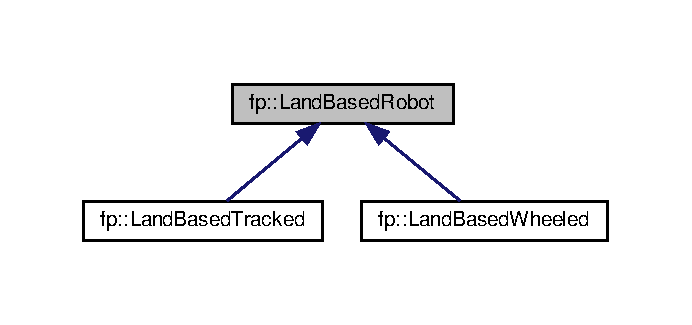
\includegraphics[width=332pt]{classfp_1_1_land_based_robot__inherit__graph}
\end{center}
\end{figure}
\subsection*{Public Member Functions}
\begin{DoxyCompactItemize}
\item 
double \hyperlink{classfp_1_1_land_based_robot_a44fed3a00505f6679ff8505aebae4505}{get\+\_\+speed} () const
\begin{DoxyCompactList}\small\item\em Accessor function for speed. \end{DoxyCompactList}\item 
double \hyperlink{classfp_1_1_land_based_robot_a523b439167030a7ab1e0e7f6c8d42315}{get\+\_\+width} () const
\begin{DoxyCompactList}\small\item\em Accessor function for width. \end{DoxyCompactList}\item 
double \hyperlink{classfp_1_1_land_based_robot_adb03fbded9a3b0553301bcc0322cb1c1}{get\+\_\+length} () const
\begin{DoxyCompactList}\small\item\em Accessor function for length. \end{DoxyCompactList}\item 
double \hyperlink{classfp_1_1_land_based_robot_ac77253c989c417ee26654541c50669d4}{get\+\_\+height} () const
\begin{DoxyCompactList}\small\item\em Accessor function for height. \end{DoxyCompactList}\item 
double \hyperlink{classfp_1_1_land_based_robot_a24c0f6d395f3dfd6bdbcf5a2a9801de1}{get\+\_\+capacity} () const
\begin{DoxyCompactList}\small\item\em Accessor function for capacity. \end{DoxyCompactList}\item 
int \hyperlink{classfp_1_1_land_based_robot_aff91a5c22ba358b888fa4939930248ce}{getX} () const
\begin{DoxyCompactList}\small\item\em Accessor function for x. \end{DoxyCompactList}\item 
int \hyperlink{classfp_1_1_land_based_robot_ac2f55928ef37240afda0773e15ad5b17}{getY} () const
\begin{DoxyCompactList}\small\item\em Accessor function for y. \end{DoxyCompactList}\item 
double \hyperlink{classfp_1_1_land_based_robot_abddbc887170ed70d2c719cfdf9fed0b7}{set\+\_\+speed} (double \hyperlink{classfp_1_1_land_based_robot_a098908304491425d6264e59d9412e696}{speed})
\item 
double \hyperlink{classfp_1_1_land_based_robot_a04fccce1e72832a761b39889b8598c63}{set\+\_\+width} (double \hyperlink{classfp_1_1_land_based_robot_a4e49ce0ab6b8b0e4a998d5ce82303f8d}{width})
\item 
double \hyperlink{classfp_1_1_land_based_robot_a7dc263eed0275d71688a2e57fe93029a}{set\+\_\+length} (double \hyperlink{classfp_1_1_land_based_robot_aa96f1f19673132a99ce0b417faed83d3}{length})
\item 
double \hyperlink{classfp_1_1_land_based_robot_a2197cbdc219c952931fe05ad707ab9ed}{set\+\_\+height} (double \hyperlink{classfp_1_1_land_based_robot_a6b1ece64bf32bbe509042ccb80a2ab33}{height})
\item 
double \hyperlink{classfp_1_1_land_based_robot_a3db2d374deb78e67c19bdf07bca9d771}{set\+\_\+capacity} (double \hyperlink{classfp_1_1_land_based_robot_af906410bad105b30865b9a02fdd350f9}{capacity})
\item 
\hyperlink{classfp_1_1_land_based_robot_a08abaf52a0b6968a8dfce230a47adca7}{Land\+Based\+Robot} (std\+::string name=\char`\"{}robot\char`\"{}, int \hyperlink{classfp_1_1_land_based_robot_a305bb45b4478ab51080fa0d7fc7bc2d7}{x}=0, int \hyperlink{classfp_1_1_land_based_robot_ad1ff889538680eba6bc6eb135b4ccd63}{y}=0, char direction=\textquotesingle{}n\textquotesingle{})
\item 
virtual char \hyperlink{classfp_1_1_land_based_robot_a50841b6e40d4e92832770d26b427fea2}{Get\+Direction} ()=0
\item 
virtual void \hyperlink{classfp_1_1_land_based_robot_a370d28ef28553e8e7a56b1ea68884bb0}{Move\+Forward} (int \hyperlink{classfp_1_1_land_based_robot_a305bb45b4478ab51080fa0d7fc7bc2d7}{x}, int \hyperlink{classfp_1_1_land_based_robot_ad1ff889538680eba6bc6eb135b4ccd63}{y}, char direction)=0
\item 
virtual void \hyperlink{classfp_1_1_land_based_robot_acd135f01e40d4f2e32739156b56c722f}{Turn\+Left} ()=0
\item 
virtual void \hyperlink{classfp_1_1_land_based_robot_aa905ba0f9b2670bea138df1e5d6836ff}{Turn\+Right} ()=0
\item 
virtual \hyperlink{classfp_1_1_land_based_robot_acfe49650459e4e6c72b87e6eff1072d9}{$\sim$\+Land\+Based\+Robot} ()
\end{DoxyCompactItemize}
\subsection*{Public Attributes}
\begin{DoxyCompactItemize}
\item 
double \hyperlink{classfp_1_1_land_based_robot_a098908304491425d6264e59d9412e696}{speed} = \hyperlink{classfp_1_1_land_based_robot_a44fed3a00505f6679ff8505aebae4505}{get\+\_\+speed}()
\item 
double \hyperlink{classfp_1_1_land_based_robot_a4e49ce0ab6b8b0e4a998d5ce82303f8d}{width} = \hyperlink{classfp_1_1_land_based_robot_a523b439167030a7ab1e0e7f6c8d42315}{get\+\_\+width}()
\item 
double \hyperlink{classfp_1_1_land_based_robot_aa96f1f19673132a99ce0b417faed83d3}{length} = \hyperlink{classfp_1_1_land_based_robot_adb03fbded9a3b0553301bcc0322cb1c1}{get\+\_\+length}()
\item 
double \hyperlink{classfp_1_1_land_based_robot_a6b1ece64bf32bbe509042ccb80a2ab33}{height} = \hyperlink{classfp_1_1_land_based_robot_ac77253c989c417ee26654541c50669d4}{get\+\_\+height}()
\item 
double \hyperlink{classfp_1_1_land_based_robot_af906410bad105b30865b9a02fdd350f9}{capacity} = \hyperlink{classfp_1_1_land_based_robot_a24c0f6d395f3dfd6bdbcf5a2a9801de1}{get\+\_\+capacity}()
\item 
int \hyperlink{classfp_1_1_land_based_robot_a305bb45b4478ab51080fa0d7fc7bc2d7}{x} = \hyperlink{classfp_1_1_land_based_robot_aff91a5c22ba358b888fa4939930248ce}{getX}()
\item 
int \hyperlink{classfp_1_1_land_based_robot_ad1ff889538680eba6bc6eb135b4ccd63}{y} = \hyperlink{classfp_1_1_land_based_robot_ac2f55928ef37240afda0773e15ad5b17}{getY}()
\end{DoxyCompactItemize}
\subsection*{Protected Attributes}
\begin{DoxyCompactItemize}
\item 
const std\+::string \hyperlink{classfp_1_1_land_based_robot_a548e8bdaead3c8ddbcaa9eac1121d1c5}{name\+\_\+}
\item 
double \hyperlink{classfp_1_1_land_based_robot_ae969157e5f910ed0a85198dc7f6c3cef}{speed\+\_\+} \{\}
\item 
double \hyperlink{classfp_1_1_land_based_robot_aae605323e9ce63f29dcded204421b1fc}{width\+\_\+} \{\}
\item 
double \hyperlink{classfp_1_1_land_based_robot_a9475d5886f329c92e68f0d86b4da58c0}{length\+\_\+} \{\}
\item 
double \hyperlink{classfp_1_1_land_based_robot_a34238a27d9055c416a3e6cfedc8ed248}{height\+\_\+} \{\}
\item 
double \hyperlink{classfp_1_1_land_based_robot_a542d90c7c62899e3c3cf28791bbb6c8e}{capacity\+\_\+} \{\}
\item 
int \hyperlink{classfp_1_1_land_based_robot_a55c2b5865fd60fb0158a135031f8b271}{x\+\_\+}
\item 
int \hyperlink{classfp_1_1_land_based_robot_a130cfd6ad383116076dc891ee3a52671}{y\+\_\+}
\item 
char \hyperlink{classfp_1_1_land_based_robot_adc8e6123fa8ffe86576e46000b0ae779}{direction\+\_\+} \{\textquotesingle{}n\textquotesingle{}\}
\end{DoxyCompactItemize}


\subsection{Constructor \& Destructor Documentation}
\mbox{\Hypertarget{classfp_1_1_land_based_robot_a08abaf52a0b6968a8dfce230a47adca7}\label{classfp_1_1_land_based_robot_a08abaf52a0b6968a8dfce230a47adca7}} 
\index{fp\+::\+Land\+Based\+Robot@{fp\+::\+Land\+Based\+Robot}!Land\+Based\+Robot@{Land\+Based\+Robot}}
\index{Land\+Based\+Robot@{Land\+Based\+Robot}!fp\+::\+Land\+Based\+Robot@{fp\+::\+Land\+Based\+Robot}}
\subsubsection{\texorpdfstring{Land\+Based\+Robot()}{LandBasedRobot()}}
{\footnotesize\ttfamily fp\+::\+Land\+Based\+Robot\+::\+Land\+Based\+Robot (\begin{DoxyParamCaption}\item[{std\+::string}]{name = {\ttfamily \char`\"{}robot\char`\"{}},  }\item[{int}]{x = {\ttfamily 0},  }\item[{int}]{y = {\ttfamily 0},  }\item[{char}]{direction = {\ttfamily \textquotesingle{}n\textquotesingle{}} }\end{DoxyParamCaption})\hspace{0.3cm}{\ttfamily [inline]}, {\ttfamily [explicit]}}

\hyperlink{classfp_1_1_land_based_robot}{Land\+Based\+Robot} Constructor 
\begin{DoxyParams}{Parameters}
{\em name} & name of the robot \\
\hline
{\em x} & x coordinate of the robot \\
\hline
{\em y} & y coordinate of the robot \\
\hline
{\em direction} & direction that the robot is facing in the maze \\
\hline
\end{DoxyParams}
\mbox{\Hypertarget{classfp_1_1_land_based_robot_acfe49650459e4e6c72b87e6eff1072d9}\label{classfp_1_1_land_based_robot_acfe49650459e4e6c72b87e6eff1072d9}} 
\index{fp\+::\+Land\+Based\+Robot@{fp\+::\+Land\+Based\+Robot}!````~Land\+Based\+Robot@{$\sim$\+Land\+Based\+Robot}}
\index{````~Land\+Based\+Robot@{$\sim$\+Land\+Based\+Robot}!fp\+::\+Land\+Based\+Robot@{fp\+::\+Land\+Based\+Robot}}
\subsubsection{\texorpdfstring{$\sim$\+Land\+Based\+Robot()}{~LandBasedRobot()}}
{\footnotesize\ttfamily virtual fp\+::\+Land\+Based\+Robot\+::$\sim$\+Land\+Based\+Robot (\begin{DoxyParamCaption}{ }\end{DoxyParamCaption})\hspace{0.3cm}{\ttfamily [inline]}, {\ttfamily [virtual]}}

$<$ Destructor for \hyperlink{classfp_1_1_land_based_robot}{Land\+Based\+Robot} 

\subsection{Member Function Documentation}
\mbox{\Hypertarget{classfp_1_1_land_based_robot_a24c0f6d395f3dfd6bdbcf5a2a9801de1}\label{classfp_1_1_land_based_robot_a24c0f6d395f3dfd6bdbcf5a2a9801de1}} 
\index{fp\+::\+Land\+Based\+Robot@{fp\+::\+Land\+Based\+Robot}!get\+\_\+capacity@{get\+\_\+capacity}}
\index{get\+\_\+capacity@{get\+\_\+capacity}!fp\+::\+Land\+Based\+Robot@{fp\+::\+Land\+Based\+Robot}}
\subsubsection{\texorpdfstring{get\+\_\+capacity()}{get\_capacity()}}
{\footnotesize\ttfamily double fp\+::\+Land\+Based\+Robot\+::get\+\_\+capacity (\begin{DoxyParamCaption}{ }\end{DoxyParamCaption}) const\hspace{0.3cm}{\ttfamily [inline]}}



Accessor function for capacity. 

\begin{DoxyReturn}{Returns}

\end{DoxyReturn}
\mbox{\Hypertarget{classfp_1_1_land_based_robot_ac77253c989c417ee26654541c50669d4}\label{classfp_1_1_land_based_robot_ac77253c989c417ee26654541c50669d4}} 
\index{fp\+::\+Land\+Based\+Robot@{fp\+::\+Land\+Based\+Robot}!get\+\_\+height@{get\+\_\+height}}
\index{get\+\_\+height@{get\+\_\+height}!fp\+::\+Land\+Based\+Robot@{fp\+::\+Land\+Based\+Robot}}
\subsubsection{\texorpdfstring{get\+\_\+height()}{get\_height()}}
{\footnotesize\ttfamily double fp\+::\+Land\+Based\+Robot\+::get\+\_\+height (\begin{DoxyParamCaption}{ }\end{DoxyParamCaption}) const\hspace{0.3cm}{\ttfamily [inline]}}



Accessor function for height. 

\begin{DoxyReturn}{Returns}
height\+\_\+ 
\end{DoxyReturn}
\mbox{\Hypertarget{classfp_1_1_land_based_robot_adb03fbded9a3b0553301bcc0322cb1c1}\label{classfp_1_1_land_based_robot_adb03fbded9a3b0553301bcc0322cb1c1}} 
\index{fp\+::\+Land\+Based\+Robot@{fp\+::\+Land\+Based\+Robot}!get\+\_\+length@{get\+\_\+length}}
\index{get\+\_\+length@{get\+\_\+length}!fp\+::\+Land\+Based\+Robot@{fp\+::\+Land\+Based\+Robot}}
\subsubsection{\texorpdfstring{get\+\_\+length()}{get\_length()}}
{\footnotesize\ttfamily double fp\+::\+Land\+Based\+Robot\+::get\+\_\+length (\begin{DoxyParamCaption}{ }\end{DoxyParamCaption}) const\hspace{0.3cm}{\ttfamily [inline]}}



Accessor function for length. 

\begin{DoxyReturn}{Returns}
length\+\_\+ 
\end{DoxyReturn}
\mbox{\Hypertarget{classfp_1_1_land_based_robot_a44fed3a00505f6679ff8505aebae4505}\label{classfp_1_1_land_based_robot_a44fed3a00505f6679ff8505aebae4505}} 
\index{fp\+::\+Land\+Based\+Robot@{fp\+::\+Land\+Based\+Robot}!get\+\_\+speed@{get\+\_\+speed}}
\index{get\+\_\+speed@{get\+\_\+speed}!fp\+::\+Land\+Based\+Robot@{fp\+::\+Land\+Based\+Robot}}
\subsubsection{\texorpdfstring{get\+\_\+speed()}{get\_speed()}}
{\footnotesize\ttfamily double fp\+::\+Land\+Based\+Robot\+::get\+\_\+speed (\begin{DoxyParamCaption}{ }\end{DoxyParamCaption}) const\hspace{0.3cm}{\ttfamily [inline]}}



Accessor function for speed. 

\begin{DoxyReturn}{Returns}
speed\+\_\+ 
\end{DoxyReturn}
\mbox{\Hypertarget{classfp_1_1_land_based_robot_a523b439167030a7ab1e0e7f6c8d42315}\label{classfp_1_1_land_based_robot_a523b439167030a7ab1e0e7f6c8d42315}} 
\index{fp\+::\+Land\+Based\+Robot@{fp\+::\+Land\+Based\+Robot}!get\+\_\+width@{get\+\_\+width}}
\index{get\+\_\+width@{get\+\_\+width}!fp\+::\+Land\+Based\+Robot@{fp\+::\+Land\+Based\+Robot}}
\subsubsection{\texorpdfstring{get\+\_\+width()}{get\_width()}}
{\footnotesize\ttfamily double fp\+::\+Land\+Based\+Robot\+::get\+\_\+width (\begin{DoxyParamCaption}{ }\end{DoxyParamCaption}) const\hspace{0.3cm}{\ttfamily [inline]}}



Accessor function for width. 

\begin{DoxyReturn}{Returns}
width\+\_\+ 
\end{DoxyReturn}
\mbox{\Hypertarget{classfp_1_1_land_based_robot_a50841b6e40d4e92832770d26b427fea2}\label{classfp_1_1_land_based_robot_a50841b6e40d4e92832770d26b427fea2}} 
\index{fp\+::\+Land\+Based\+Robot@{fp\+::\+Land\+Based\+Robot}!Get\+Direction@{Get\+Direction}}
\index{Get\+Direction@{Get\+Direction}!fp\+::\+Land\+Based\+Robot@{fp\+::\+Land\+Based\+Robot}}
\subsubsection{\texorpdfstring{Get\+Direction()}{GetDirection()}}
{\footnotesize\ttfamily char fp\+::\+Land\+Based\+Robot\+::\+Get\+Direction (\begin{DoxyParamCaption}{ }\end{DoxyParamCaption})\hspace{0.3cm}{\ttfamily [pure virtual]}}

Virtual Get\+Direction Method Get the direction of the robot in the maze 
\begin{DoxyParams}{Parameters}
{\em x} & x coordinate of the robot \\
\hline
{\em y} & y coordinate of the robot \\
\hline
\end{DoxyParams}


Implemented in \hyperlink{classfp_1_1_land_based_tracked_a3e6ba37a5c5bf8f2b4abb19907e5e9b8}{fp\+::\+Land\+Based\+Tracked}, and \hyperlink{classfp_1_1_land_based_wheeled_adaafaceb388374ffb9cec28301665492}{fp\+::\+Land\+Based\+Wheeled}.

\mbox{\Hypertarget{classfp_1_1_land_based_robot_aff91a5c22ba358b888fa4939930248ce}\label{classfp_1_1_land_based_robot_aff91a5c22ba358b888fa4939930248ce}} 
\index{fp\+::\+Land\+Based\+Robot@{fp\+::\+Land\+Based\+Robot}!getX@{getX}}
\index{getX@{getX}!fp\+::\+Land\+Based\+Robot@{fp\+::\+Land\+Based\+Robot}}
\subsubsection{\texorpdfstring{get\+X()}{getX()}}
{\footnotesize\ttfamily int fp\+::\+Land\+Based\+Robot\+::getX (\begin{DoxyParamCaption}{ }\end{DoxyParamCaption}) const\hspace{0.3cm}{\ttfamily [inline]}}



Accessor function for x. 

\begin{DoxyReturn}{Returns}
none 
\end{DoxyReturn}
\mbox{\Hypertarget{classfp_1_1_land_based_robot_ac2f55928ef37240afda0773e15ad5b17}\label{classfp_1_1_land_based_robot_ac2f55928ef37240afda0773e15ad5b17}} 
\index{fp\+::\+Land\+Based\+Robot@{fp\+::\+Land\+Based\+Robot}!getY@{getY}}
\index{getY@{getY}!fp\+::\+Land\+Based\+Robot@{fp\+::\+Land\+Based\+Robot}}
\subsubsection{\texorpdfstring{get\+Y()}{getY()}}
{\footnotesize\ttfamily int fp\+::\+Land\+Based\+Robot\+::getY (\begin{DoxyParamCaption}{ }\end{DoxyParamCaption}) const\hspace{0.3cm}{\ttfamily [inline]}}



Accessor function for y. 

\begin{DoxyReturn}{Returns}
none 
\end{DoxyReturn}
\mbox{\Hypertarget{classfp_1_1_land_based_robot_a370d28ef28553e8e7a56b1ea68884bb0}\label{classfp_1_1_land_based_robot_a370d28ef28553e8e7a56b1ea68884bb0}} 
\index{fp\+::\+Land\+Based\+Robot@{fp\+::\+Land\+Based\+Robot}!Move\+Forward@{Move\+Forward}}
\index{Move\+Forward@{Move\+Forward}!fp\+::\+Land\+Based\+Robot@{fp\+::\+Land\+Based\+Robot}}
\subsubsection{\texorpdfstring{Move\+Forward()}{MoveForward()}}
{\footnotesize\ttfamily void fp\+::\+Land\+Based\+Robot\+::\+Move\+Forward (\begin{DoxyParamCaption}\item[{int}]{x,  }\item[{int}]{y,  }\item[{char}]{direction }\end{DoxyParamCaption})\hspace{0.3cm}{\ttfamily [pure virtual]}}

Virtual Move\+Forward Method Moves the robot forward in the maze 
\begin{DoxyParams}{Parameters}
{\em x} & x coordinate of the robot \\
\hline
{\em y} & y coordinate of the robot \\
\hline
\end{DoxyParams}


Implemented in \hyperlink{classfp_1_1_land_based_tracked_a3f4290b614fe0e31e361366e71501cea}{fp\+::\+Land\+Based\+Tracked}, and \hyperlink{classfp_1_1_land_based_wheeled_a90ab977baecc518185c950b08c56dfc5}{fp\+::\+Land\+Based\+Wheeled}.

\mbox{\Hypertarget{classfp_1_1_land_based_robot_a3db2d374deb78e67c19bdf07bca9d771}\label{classfp_1_1_land_based_robot_a3db2d374deb78e67c19bdf07bca9d771}} 
\index{fp\+::\+Land\+Based\+Robot@{fp\+::\+Land\+Based\+Robot}!set\+\_\+capacity@{set\+\_\+capacity}}
\index{set\+\_\+capacity@{set\+\_\+capacity}!fp\+::\+Land\+Based\+Robot@{fp\+::\+Land\+Based\+Robot}}
\subsubsection{\texorpdfstring{set\+\_\+capacity()}{set\_capacity()}}
{\footnotesize\ttfamily double fp\+::\+Land\+Based\+Robot\+::set\+\_\+capacity (\begin{DoxyParamCaption}\item[{double}]{capacity }\end{DoxyParamCaption})\hspace{0.3cm}{\ttfamily [inline]}}

Mutator (setter) function for capacity 
\begin{DoxyParams}{Parameters}
{\em capacity} & \\
\hline
\end{DoxyParams}
\begin{DoxyReturn}{Returns}

\end{DoxyReturn}
\mbox{\Hypertarget{classfp_1_1_land_based_robot_a2197cbdc219c952931fe05ad707ab9ed}\label{classfp_1_1_land_based_robot_a2197cbdc219c952931fe05ad707ab9ed}} 
\index{fp\+::\+Land\+Based\+Robot@{fp\+::\+Land\+Based\+Robot}!set\+\_\+height@{set\+\_\+height}}
\index{set\+\_\+height@{set\+\_\+height}!fp\+::\+Land\+Based\+Robot@{fp\+::\+Land\+Based\+Robot}}
\subsubsection{\texorpdfstring{set\+\_\+height()}{set\_height()}}
{\footnotesize\ttfamily double fp\+::\+Land\+Based\+Robot\+::set\+\_\+height (\begin{DoxyParamCaption}\item[{double}]{height }\end{DoxyParamCaption})\hspace{0.3cm}{\ttfamily [inline]}}

Mutator (setter) function for height 
\begin{DoxyParams}{Parameters}
{\em height} & \\
\hline
\end{DoxyParams}
\begin{DoxyReturn}{Returns}

\end{DoxyReturn}
\mbox{\Hypertarget{classfp_1_1_land_based_robot_a7dc263eed0275d71688a2e57fe93029a}\label{classfp_1_1_land_based_robot_a7dc263eed0275d71688a2e57fe93029a}} 
\index{fp\+::\+Land\+Based\+Robot@{fp\+::\+Land\+Based\+Robot}!set\+\_\+length@{set\+\_\+length}}
\index{set\+\_\+length@{set\+\_\+length}!fp\+::\+Land\+Based\+Robot@{fp\+::\+Land\+Based\+Robot}}
\subsubsection{\texorpdfstring{set\+\_\+length()}{set\_length()}}
{\footnotesize\ttfamily double fp\+::\+Land\+Based\+Robot\+::set\+\_\+length (\begin{DoxyParamCaption}\item[{double}]{length }\end{DoxyParamCaption})\hspace{0.3cm}{\ttfamily [inline]}}

Mutator (setter) function for length 
\begin{DoxyParams}{Parameters}
{\em length} & \\
\hline
\end{DoxyParams}
\begin{DoxyReturn}{Returns}

\end{DoxyReturn}
\mbox{\Hypertarget{classfp_1_1_land_based_robot_abddbc887170ed70d2c719cfdf9fed0b7}\label{classfp_1_1_land_based_robot_abddbc887170ed70d2c719cfdf9fed0b7}} 
\index{fp\+::\+Land\+Based\+Robot@{fp\+::\+Land\+Based\+Robot}!set\+\_\+speed@{set\+\_\+speed}}
\index{set\+\_\+speed@{set\+\_\+speed}!fp\+::\+Land\+Based\+Robot@{fp\+::\+Land\+Based\+Robot}}
\subsubsection{\texorpdfstring{set\+\_\+speed()}{set\_speed()}}
{\footnotesize\ttfamily double fp\+::\+Land\+Based\+Robot\+::set\+\_\+speed (\begin{DoxyParamCaption}\item[{double}]{speed }\end{DoxyParamCaption})\hspace{0.3cm}{\ttfamily [inline]}}

Mutator (setter) function for speed 
\begin{DoxyParams}{Parameters}
{\em speed} & \\
\hline
\end{DoxyParams}
\begin{DoxyReturn}{Returns}
Returns nothing 
\end{DoxyReturn}
\mbox{\Hypertarget{classfp_1_1_land_based_robot_a04fccce1e72832a761b39889b8598c63}\label{classfp_1_1_land_based_robot_a04fccce1e72832a761b39889b8598c63}} 
\index{fp\+::\+Land\+Based\+Robot@{fp\+::\+Land\+Based\+Robot}!set\+\_\+width@{set\+\_\+width}}
\index{set\+\_\+width@{set\+\_\+width}!fp\+::\+Land\+Based\+Robot@{fp\+::\+Land\+Based\+Robot}}
\subsubsection{\texorpdfstring{set\+\_\+width()}{set\_width()}}
{\footnotesize\ttfamily double fp\+::\+Land\+Based\+Robot\+::set\+\_\+width (\begin{DoxyParamCaption}\item[{double}]{width }\end{DoxyParamCaption})\hspace{0.3cm}{\ttfamily [inline]}}

Mutator (setter) function for width 
\begin{DoxyParams}{Parameters}
{\em width} & \\
\hline
\end{DoxyParams}
\begin{DoxyReturn}{Returns}

\end{DoxyReturn}
\mbox{\Hypertarget{classfp_1_1_land_based_robot_acd135f01e40d4f2e32739156b56c722f}\label{classfp_1_1_land_based_robot_acd135f01e40d4f2e32739156b56c722f}} 
\index{fp\+::\+Land\+Based\+Robot@{fp\+::\+Land\+Based\+Robot}!Turn\+Left@{Turn\+Left}}
\index{Turn\+Left@{Turn\+Left}!fp\+::\+Land\+Based\+Robot@{fp\+::\+Land\+Based\+Robot}}
\subsubsection{\texorpdfstring{Turn\+Left()}{TurnLeft()}}
{\footnotesize\ttfamily void fp\+::\+Land\+Based\+Robot\+::\+Turn\+Left (\begin{DoxyParamCaption}{ }\end{DoxyParamCaption})\hspace{0.3cm}{\ttfamily [pure virtual]}}

Turn\+Left Method Rotate the the robot 90 degrees counter-\/clockwise 

Implemented in \hyperlink{classfp_1_1_land_based_tracked_a63141c32f8f81c301be4126297103a41}{fp\+::\+Land\+Based\+Tracked}, and \hyperlink{classfp_1_1_land_based_wheeled_a240c5e9cf72006ac2f99f8e1dfc4dc5d}{fp\+::\+Land\+Based\+Wheeled}.

\mbox{\Hypertarget{classfp_1_1_land_based_robot_aa905ba0f9b2670bea138df1e5d6836ff}\label{classfp_1_1_land_based_robot_aa905ba0f9b2670bea138df1e5d6836ff}} 
\index{fp\+::\+Land\+Based\+Robot@{fp\+::\+Land\+Based\+Robot}!Turn\+Right@{Turn\+Right}}
\index{Turn\+Right@{Turn\+Right}!fp\+::\+Land\+Based\+Robot@{fp\+::\+Land\+Based\+Robot}}
\subsubsection{\texorpdfstring{Turn\+Right()}{TurnRight()}}
{\footnotesize\ttfamily void fp\+::\+Land\+Based\+Robot\+::\+Turn\+Right (\begin{DoxyParamCaption}{ }\end{DoxyParamCaption})\hspace{0.3cm}{\ttfamily [pure virtual]}}

Turn\+Right Method Rotate the the robot 90 degrees clockwise 

Implemented in \hyperlink{classfp_1_1_land_based_tracked_a813613a1eaa7a0782ea254a167d97da3}{fp\+::\+Land\+Based\+Tracked}, and \hyperlink{classfp_1_1_land_based_wheeled_a505f5c33f04681aa5c7362531947f4ca}{fp\+::\+Land\+Based\+Wheeled}.



\subsection{Member Data Documentation}
\mbox{\Hypertarget{classfp_1_1_land_based_robot_af906410bad105b30865b9a02fdd350f9}\label{classfp_1_1_land_based_robot_af906410bad105b30865b9a02fdd350f9}} 
\index{fp\+::\+Land\+Based\+Robot@{fp\+::\+Land\+Based\+Robot}!capacity@{capacity}}
\index{capacity@{capacity}!fp\+::\+Land\+Based\+Robot@{fp\+::\+Land\+Based\+Robot}}
\subsubsection{\texorpdfstring{capacity}{capacity}}
{\footnotesize\ttfamily double fp\+::\+Land\+Based\+Robot\+::capacity = \hyperlink{classfp_1_1_land_based_robot_a24c0f6d395f3dfd6bdbcf5a2a9801de1}{get\+\_\+capacity}()}

\mbox{\Hypertarget{classfp_1_1_land_based_robot_a542d90c7c62899e3c3cf28791bbb6c8e}\label{classfp_1_1_land_based_robot_a542d90c7c62899e3c3cf28791bbb6c8e}} 
\index{fp\+::\+Land\+Based\+Robot@{fp\+::\+Land\+Based\+Robot}!capacity\+\_\+@{capacity\+\_\+}}
\index{capacity\+\_\+@{capacity\+\_\+}!fp\+::\+Land\+Based\+Robot@{fp\+::\+Land\+Based\+Robot}}
\subsubsection{\texorpdfstring{capacity\+\_\+}{capacity\_}}
{\footnotesize\ttfamily double fp\+::\+Land\+Based\+Robot\+::capacity\+\_\+ \{\}\hspace{0.3cm}{\ttfamily [protected]}}

Height of the base of the robot \mbox{\Hypertarget{classfp_1_1_land_based_robot_adc8e6123fa8ffe86576e46000b0ae779}\label{classfp_1_1_land_based_robot_adc8e6123fa8ffe86576e46000b0ae779}} 
\index{fp\+::\+Land\+Based\+Robot@{fp\+::\+Land\+Based\+Robot}!direction\+\_\+@{direction\+\_\+}}
\index{direction\+\_\+@{direction\+\_\+}!fp\+::\+Land\+Based\+Robot@{fp\+::\+Land\+Based\+Robot}}
\subsubsection{\texorpdfstring{direction\+\_\+}{direction\_}}
{\footnotesize\ttfamily char fp\+::\+Land\+Based\+Robot\+::direction\+\_\+ \{\textquotesingle{}n\textquotesingle{}\}\hspace{0.3cm}{\ttfamily [protected]}}

Direction that the robot is facing in the maze \mbox{\Hypertarget{classfp_1_1_land_based_robot_a6b1ece64bf32bbe509042ccb80a2ab33}\label{classfp_1_1_land_based_robot_a6b1ece64bf32bbe509042ccb80a2ab33}} 
\index{fp\+::\+Land\+Based\+Robot@{fp\+::\+Land\+Based\+Robot}!height@{height}}
\index{height@{height}!fp\+::\+Land\+Based\+Robot@{fp\+::\+Land\+Based\+Robot}}
\subsubsection{\texorpdfstring{height}{height}}
{\footnotesize\ttfamily double fp\+::\+Land\+Based\+Robot\+::height = \hyperlink{classfp_1_1_land_based_robot_ac77253c989c417ee26654541c50669d4}{get\+\_\+height}()}

\mbox{\Hypertarget{classfp_1_1_land_based_robot_a34238a27d9055c416a3e6cfedc8ed248}\label{classfp_1_1_land_based_robot_a34238a27d9055c416a3e6cfedc8ed248}} 
\index{fp\+::\+Land\+Based\+Robot@{fp\+::\+Land\+Based\+Robot}!height\+\_\+@{height\+\_\+}}
\index{height\+\_\+@{height\+\_\+}!fp\+::\+Land\+Based\+Robot@{fp\+::\+Land\+Based\+Robot}}
\subsubsection{\texorpdfstring{height\+\_\+}{height\_}}
{\footnotesize\ttfamily double fp\+::\+Land\+Based\+Robot\+::height\+\_\+ \{\}\hspace{0.3cm}{\ttfamily [protected]}}

Height of the base of the robot \mbox{\Hypertarget{classfp_1_1_land_based_robot_aa96f1f19673132a99ce0b417faed83d3}\label{classfp_1_1_land_based_robot_aa96f1f19673132a99ce0b417faed83d3}} 
\index{fp\+::\+Land\+Based\+Robot@{fp\+::\+Land\+Based\+Robot}!length@{length}}
\index{length@{length}!fp\+::\+Land\+Based\+Robot@{fp\+::\+Land\+Based\+Robot}}
\subsubsection{\texorpdfstring{length}{length}}
{\footnotesize\ttfamily double fp\+::\+Land\+Based\+Robot\+::length = \hyperlink{classfp_1_1_land_based_robot_adb03fbded9a3b0553301bcc0322cb1c1}{get\+\_\+length}()}

\mbox{\Hypertarget{classfp_1_1_land_based_robot_a9475d5886f329c92e68f0d86b4da58c0}\label{classfp_1_1_land_based_robot_a9475d5886f329c92e68f0d86b4da58c0}} 
\index{fp\+::\+Land\+Based\+Robot@{fp\+::\+Land\+Based\+Robot}!length\+\_\+@{length\+\_\+}}
\index{length\+\_\+@{length\+\_\+}!fp\+::\+Land\+Based\+Robot@{fp\+::\+Land\+Based\+Robot}}
\subsubsection{\texorpdfstring{length\+\_\+}{length\_}}
{\footnotesize\ttfamily double fp\+::\+Land\+Based\+Robot\+::length\+\_\+ \{\}\hspace{0.3cm}{\ttfamily [protected]}}

Width of the base of the robot \mbox{\Hypertarget{classfp_1_1_land_based_robot_a548e8bdaead3c8ddbcaa9eac1121d1c5}\label{classfp_1_1_land_based_robot_a548e8bdaead3c8ddbcaa9eac1121d1c5}} 
\index{fp\+::\+Land\+Based\+Robot@{fp\+::\+Land\+Based\+Robot}!name\+\_\+@{name\+\_\+}}
\index{name\+\_\+@{name\+\_\+}!fp\+::\+Land\+Based\+Robot@{fp\+::\+Land\+Based\+Robot}}
\subsubsection{\texorpdfstring{name\+\_\+}{name\_}}
{\footnotesize\ttfamily const std\+::string fp\+::\+Land\+Based\+Robot\+::name\+\_\+\hspace{0.3cm}{\ttfamily [protected]}}

$<$ Attributes Name of the robot \mbox{\Hypertarget{classfp_1_1_land_based_robot_a098908304491425d6264e59d9412e696}\label{classfp_1_1_land_based_robot_a098908304491425d6264e59d9412e696}} 
\index{fp\+::\+Land\+Based\+Robot@{fp\+::\+Land\+Based\+Robot}!speed@{speed}}
\index{speed@{speed}!fp\+::\+Land\+Based\+Robot@{fp\+::\+Land\+Based\+Robot}}
\subsubsection{\texorpdfstring{speed}{speed}}
{\footnotesize\ttfamily double fp\+::\+Land\+Based\+Robot\+::speed = \hyperlink{classfp_1_1_land_based_robot_a44fed3a00505f6679ff8505aebae4505}{get\+\_\+speed}()}

\mbox{\Hypertarget{classfp_1_1_land_based_robot_ae969157e5f910ed0a85198dc7f6c3cef}\label{classfp_1_1_land_based_robot_ae969157e5f910ed0a85198dc7f6c3cef}} 
\index{fp\+::\+Land\+Based\+Robot@{fp\+::\+Land\+Based\+Robot}!speed\+\_\+@{speed\+\_\+}}
\index{speed\+\_\+@{speed\+\_\+}!fp\+::\+Land\+Based\+Robot@{fp\+::\+Land\+Based\+Robot}}
\subsubsection{\texorpdfstring{speed\+\_\+}{speed\_}}
{\footnotesize\ttfamily double fp\+::\+Land\+Based\+Robot\+::speed\+\_\+ \{\}\hspace{0.3cm}{\ttfamily [protected]}}

Driving speed of the robot \mbox{\Hypertarget{classfp_1_1_land_based_robot_a4e49ce0ab6b8b0e4a998d5ce82303f8d}\label{classfp_1_1_land_based_robot_a4e49ce0ab6b8b0e4a998d5ce82303f8d}} 
\index{fp\+::\+Land\+Based\+Robot@{fp\+::\+Land\+Based\+Robot}!width@{width}}
\index{width@{width}!fp\+::\+Land\+Based\+Robot@{fp\+::\+Land\+Based\+Robot}}
\subsubsection{\texorpdfstring{width}{width}}
{\footnotesize\ttfamily double fp\+::\+Land\+Based\+Robot\+::width = \hyperlink{classfp_1_1_land_based_robot_a523b439167030a7ab1e0e7f6c8d42315}{get\+\_\+width}()}

\mbox{\Hypertarget{classfp_1_1_land_based_robot_aae605323e9ce63f29dcded204421b1fc}\label{classfp_1_1_land_based_robot_aae605323e9ce63f29dcded204421b1fc}} 
\index{fp\+::\+Land\+Based\+Robot@{fp\+::\+Land\+Based\+Robot}!width\+\_\+@{width\+\_\+}}
\index{width\+\_\+@{width\+\_\+}!fp\+::\+Land\+Based\+Robot@{fp\+::\+Land\+Based\+Robot}}
\subsubsection{\texorpdfstring{width\+\_\+}{width\_}}
{\footnotesize\ttfamily double fp\+::\+Land\+Based\+Robot\+::width\+\_\+ \{\}\hspace{0.3cm}{\ttfamily [protected]}}

Width of the base of the robot \mbox{\Hypertarget{classfp_1_1_land_based_robot_a305bb45b4478ab51080fa0d7fc7bc2d7}\label{classfp_1_1_land_based_robot_a305bb45b4478ab51080fa0d7fc7bc2d7}} 
\index{fp\+::\+Land\+Based\+Robot@{fp\+::\+Land\+Based\+Robot}!x@{x}}
\index{x@{x}!fp\+::\+Land\+Based\+Robot@{fp\+::\+Land\+Based\+Robot}}
\subsubsection{\texorpdfstring{x}{x}}
{\footnotesize\ttfamily int fp\+::\+Land\+Based\+Robot\+::x = \hyperlink{classfp_1_1_land_based_robot_aff91a5c22ba358b888fa4939930248ce}{getX}()}

\mbox{\Hypertarget{classfp_1_1_land_based_robot_a55c2b5865fd60fb0158a135031f8b271}\label{classfp_1_1_land_based_robot_a55c2b5865fd60fb0158a135031f8b271}} 
\index{fp\+::\+Land\+Based\+Robot@{fp\+::\+Land\+Based\+Robot}!x\+\_\+@{x\+\_\+}}
\index{x\+\_\+@{x\+\_\+}!fp\+::\+Land\+Based\+Robot@{fp\+::\+Land\+Based\+Robot}}
\subsubsection{\texorpdfstring{x\+\_\+}{x\_}}
{\footnotesize\ttfamily int fp\+::\+Land\+Based\+Robot\+::x\+\_\+\hspace{0.3cm}{\ttfamily [protected]}}

x coordinate of the robot \mbox{\Hypertarget{classfp_1_1_land_based_robot_ad1ff889538680eba6bc6eb135b4ccd63}\label{classfp_1_1_land_based_robot_ad1ff889538680eba6bc6eb135b4ccd63}} 
\index{fp\+::\+Land\+Based\+Robot@{fp\+::\+Land\+Based\+Robot}!y@{y}}
\index{y@{y}!fp\+::\+Land\+Based\+Robot@{fp\+::\+Land\+Based\+Robot}}
\subsubsection{\texorpdfstring{y}{y}}
{\footnotesize\ttfamily int fp\+::\+Land\+Based\+Robot\+::y = \hyperlink{classfp_1_1_land_based_robot_ac2f55928ef37240afda0773e15ad5b17}{getY}()}

\mbox{\Hypertarget{classfp_1_1_land_based_robot_a130cfd6ad383116076dc891ee3a52671}\label{classfp_1_1_land_based_robot_a130cfd6ad383116076dc891ee3a52671}} 
\index{fp\+::\+Land\+Based\+Robot@{fp\+::\+Land\+Based\+Robot}!y\+\_\+@{y\+\_\+}}
\index{y\+\_\+@{y\+\_\+}!fp\+::\+Land\+Based\+Robot@{fp\+::\+Land\+Based\+Robot}}
\subsubsection{\texorpdfstring{y\+\_\+}{y\_}}
{\footnotesize\ttfamily int fp\+::\+Land\+Based\+Robot\+::y\+\_\+\hspace{0.3cm}{\ttfamily [protected]}}

y coordinate of the robot 

The documentation for this class was generated from the following files\+:\begin{DoxyCompactItemize}
\item 
/home/diane/\+One\+Drive/\+Fall 2020/\+E\+N\+P\+M809\+Y Intro Robot Programming/\+Homework/\+Final-\/\+Project-\/\+Group3/src/\+Land\+Based\+Robot/\hyperlink{_land_based_robot_8h}{Land\+Based\+Robot.\+h}\item 
/home/diane/\+One\+Drive/\+Fall 2020/\+E\+N\+P\+M809\+Y Intro Robot Programming/\+Homework/\+Final-\/\+Project-\/\+Group3/src/\+Land\+Based\+Robot/\hyperlink{_land_based_robot_8cpp}{Land\+Based\+Robot.\+cpp}\end{DoxyCompactItemize}

\hypertarget{classfp_1_1_land_based_tracked}{}\section{fp\+:\+:Land\+Based\+Tracked Class Reference}
\label{classfp_1_1_land_based_tracked}\index{fp\+::\+Land\+Based\+Tracked@{fp\+::\+Land\+Based\+Tracked}}


{\ttfamily \#include $<$landbasedtracked.\+h$>$}



Inheritance diagram for fp\+:\+:Land\+Based\+Tracked\+:\nopagebreak
\begin{figure}[H]
\begin{center}
\leavevmode
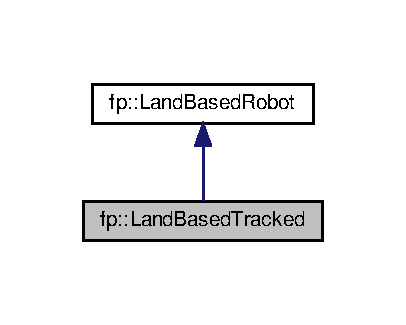
\includegraphics[width=195pt]{classfp_1_1_land_based_tracked__inherit__graph}
\end{center}
\end{figure}


Collaboration diagram for fp\+:\+:Land\+Based\+Tracked\+:\nopagebreak
\begin{figure}[H]
\begin{center}
\leavevmode
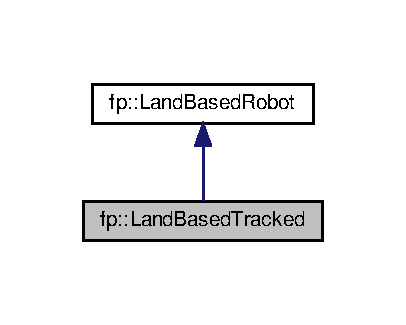
\includegraphics[width=195pt]{classfp_1_1_land_based_tracked__coll__graph}
\end{center}
\end{figure}
\subsection*{Public Member Functions}
\begin{DoxyCompactItemize}
\item 
\hyperlink{classfp_1_1_land_based_tracked_adde9b81138a39b13b4b05386c1a6b3a3}{Land\+Based\+Tracked} (std\+::string name=\char`\"{}tracked\char`\"{}, int \hyperlink{classfp_1_1_land_based_robot_a305bb45b4478ab51080fa0d7fc7bc2d7}{x}=0, int \hyperlink{classfp_1_1_land_based_robot_ad1ff889538680eba6bc6eb135b4ccd63}{y}=0, char direction=\textquotesingle{}N\textquotesingle{})
\item 
virtual char \hyperlink{classfp_1_1_land_based_tracked_a3e6ba37a5c5bf8f2b4abb19907e5e9b8}{Get\+Direction} () override
\item 
virtual void \hyperlink{classfp_1_1_land_based_tracked_a3f4290b614fe0e31e361366e71501cea}{Move\+Forward} (int \hyperlink{classfp_1_1_land_based_robot_a305bb45b4478ab51080fa0d7fc7bc2d7}{x}, int \hyperlink{classfp_1_1_land_based_robot_ad1ff889538680eba6bc6eb135b4ccd63}{y}, char direction) override
\item 
void \hyperlink{classfp_1_1_land_based_tracked_a63141c32f8f81c301be4126297103a41}{Turn\+Left} () override
\item 
void \hyperlink{classfp_1_1_land_based_tracked_a813613a1eaa7a0782ea254a167d97da3}{Turn\+Right} () override
\item 
virtual \hyperlink{classfp_1_1_land_based_tracked_a60b4e1da43f053a5a0351d52d79785e0}{$\sim$\+Land\+Based\+Tracked} ()
\end{DoxyCompactItemize}
\subsection*{Public Attributes}
\begin{DoxyCompactItemize}
\item 
double \hyperlink{classfp_1_1_land_based_tracked_a08b67f2f7c1da6db1c4d6cf4de689573}{speed} = \hyperlink{classfp_1_1_land_based_robot_a44fed3a00505f6679ff8505aebae4505}{Land\+Based\+Robot\+::get\+\_\+speed}()
\item 
double \hyperlink{classfp_1_1_land_based_tracked_a82b74ecf56d8d84b001fcb4f1ae92dad}{width} = \hyperlink{classfp_1_1_land_based_robot_a523b439167030a7ab1e0e7f6c8d42315}{Land\+Based\+Robot\+::get\+\_\+width}()
\item 
double \hyperlink{classfp_1_1_land_based_tracked_a5c81a68468defb336f0c207069290cc2}{length} = \hyperlink{classfp_1_1_land_based_robot_adb03fbded9a3b0553301bcc0322cb1c1}{Land\+Based\+Robot\+::get\+\_\+length}()
\item 
double \hyperlink{classfp_1_1_land_based_tracked_a23bbcb88d1b14513c786017dc1ceee66}{height} = \hyperlink{classfp_1_1_land_based_robot_ac77253c989c417ee26654541c50669d4}{Land\+Based\+Robot\+::get\+\_\+height}()
\item 
double \hyperlink{classfp_1_1_land_based_tracked_a13d92f0fa31949ca268678a7c339d4f7}{capacity} = \hyperlink{classfp_1_1_land_based_robot_a24c0f6d395f3dfd6bdbcf5a2a9801de1}{Land\+Based\+Robot\+::get\+\_\+capacity}()
\end{DoxyCompactItemize}
\subsection*{Protected Attributes}
\begin{DoxyCompactItemize}
\item 
std\+::shared\+\_\+ptr$<$ std\+::string $>$ \hyperlink{classfp_1_1_land_based_tracked_a2e5f75cdd135af0f33a369058de3b15c}{track\+\_\+type\+\_\+}
\item 
const std\+::string \hyperlink{classfp_1_1_land_based_tracked_abf54193cc934e3e3833a2ed3767eee9a}{name\+\_\+}
\item 
double \hyperlink{classfp_1_1_land_based_tracked_ae4203781ac58381e57fe189d6bf9908a}{speed\+\_\+} \{\}
\item 
double \hyperlink{classfp_1_1_land_based_tracked_ac3f7d3a782facd141e5a604a6ba150f8}{width\+\_\+} \{\}
\item 
double \hyperlink{classfp_1_1_land_based_tracked_ab6a7476275dfee103cfd8b1f5817d79a}{length\+\_\+} \{\}
\item 
double \hyperlink{classfp_1_1_land_based_tracked_a5f9e0d15ade5738525ccef9d8899a1b2}{height\+\_\+} \{\}
\item 
double \hyperlink{classfp_1_1_land_based_tracked_a608f59273d6f0882809fa11dbb1ca325}{capacity\+\_\+} \{\}
\item 
int \hyperlink{classfp_1_1_land_based_tracked_a8001133ebf0739a851c283248b7bf3f3}{x\+\_\+} \{\}
\item 
int \hyperlink{classfp_1_1_land_based_tracked_ae8f41c1bd340a84c7704b3bd7281ae79}{y\+\_\+} \{\}
\item 
char \hyperlink{classfp_1_1_land_based_tracked_a2efd39a637cc76891f6e8fd1eb84420e}{direction\+\_\+} \{\textquotesingle{}N\textquotesingle{}\}
\end{DoxyCompactItemize}


\subsection{Constructor \& Destructor Documentation}
\mbox{\Hypertarget{classfp_1_1_land_based_tracked_adde9b81138a39b13b4b05386c1a6b3a3}\label{classfp_1_1_land_based_tracked_adde9b81138a39b13b4b05386c1a6b3a3}} 
\index{fp\+::\+Land\+Based\+Tracked@{fp\+::\+Land\+Based\+Tracked}!Land\+Based\+Tracked@{Land\+Based\+Tracked}}
\index{Land\+Based\+Tracked@{Land\+Based\+Tracked}!fp\+::\+Land\+Based\+Tracked@{fp\+::\+Land\+Based\+Tracked}}
\subsubsection{\texorpdfstring{Land\+Based\+Tracked()}{LandBasedTracked()}}
{\footnotesize\ttfamily fp\+::\+Land\+Based\+Tracked\+::\+Land\+Based\+Tracked (\begin{DoxyParamCaption}\item[{std\+::string}]{name = {\ttfamily \char`\"{}tracked\char`\"{}},  }\item[{int}]{x = {\ttfamily 0},  }\item[{int}]{y = {\ttfamily 0},  }\item[{char}]{direction = {\ttfamily \textquotesingle{}N\textquotesingle{}} }\end{DoxyParamCaption})\hspace{0.3cm}{\ttfamily [inline]}, {\ttfamily [explicit]}}

\hyperlink{classfp_1_1_land_based_tracked}{Land\+Based\+Tracked} Constructor 
\begin{DoxyParams}{Parameters}
{\em name} & name of the robot \\
\hline
{\em x} & x coordinate of the robot \\
\hline
{\em y} & y coordinate of the robot \\
\hline
{\em direction} & direction that the robot is facing in the maze \\
\hline
\end{DoxyParams}
\mbox{\Hypertarget{classfp_1_1_land_based_tracked_a60b4e1da43f053a5a0351d52d79785e0}\label{classfp_1_1_land_based_tracked_a60b4e1da43f053a5a0351d52d79785e0}} 
\index{fp\+::\+Land\+Based\+Tracked@{fp\+::\+Land\+Based\+Tracked}!````~Land\+Based\+Tracked@{$\sim$\+Land\+Based\+Tracked}}
\index{````~Land\+Based\+Tracked@{$\sim$\+Land\+Based\+Tracked}!fp\+::\+Land\+Based\+Tracked@{fp\+::\+Land\+Based\+Tracked}}
\subsubsection{\texorpdfstring{$\sim$\+Land\+Based\+Tracked()}{~LandBasedTracked()}}
{\footnotesize\ttfamily virtual fp\+::\+Land\+Based\+Tracked\+::$\sim$\+Land\+Based\+Tracked (\begin{DoxyParamCaption}{ }\end{DoxyParamCaption})\hspace{0.3cm}{\ttfamily [inline]}, {\ttfamily [virtual]}}



\subsection{Member Function Documentation}
\mbox{\Hypertarget{classfp_1_1_land_based_tracked_a3e6ba37a5c5bf8f2b4abb19907e5e9b8}\label{classfp_1_1_land_based_tracked_a3e6ba37a5c5bf8f2b4abb19907e5e9b8}} 
\index{fp\+::\+Land\+Based\+Tracked@{fp\+::\+Land\+Based\+Tracked}!Get\+Direction@{Get\+Direction}}
\index{Get\+Direction@{Get\+Direction}!fp\+::\+Land\+Based\+Tracked@{fp\+::\+Land\+Based\+Tracked}}
\subsubsection{\texorpdfstring{Get\+Direction()}{GetDirection()}}
{\footnotesize\ttfamily char fp\+::\+Land\+Based\+Tracked\+::\+Get\+Direction (\begin{DoxyParamCaption}{ }\end{DoxyParamCaption})\hspace{0.3cm}{\ttfamily [override]}, {\ttfamily [virtual]}}

Virtual Get\+Direction Method Get the direction of the robot in the maze 
\begin{DoxyParams}{Parameters}
{\em x} & x coordinate of the robot \\
\hline
{\em y} & y coordinate of the robot \\
\hline
\end{DoxyParams}


Implements \hyperlink{classfp_1_1_land_based_robot_a50841b6e40d4e92832770d26b427fea2}{fp\+::\+Land\+Based\+Robot}.

\mbox{\Hypertarget{classfp_1_1_land_based_tracked_a3f4290b614fe0e31e361366e71501cea}\label{classfp_1_1_land_based_tracked_a3f4290b614fe0e31e361366e71501cea}} 
\index{fp\+::\+Land\+Based\+Tracked@{fp\+::\+Land\+Based\+Tracked}!Move\+Forward@{Move\+Forward}}
\index{Move\+Forward@{Move\+Forward}!fp\+::\+Land\+Based\+Tracked@{fp\+::\+Land\+Based\+Tracked}}
\subsubsection{\texorpdfstring{Move\+Forward()}{MoveForward()}}
{\footnotesize\ttfamily void fp\+::\+Land\+Based\+Tracked\+::\+Move\+Forward (\begin{DoxyParamCaption}\item[{int}]{x,  }\item[{int}]{y,  }\item[{char}]{direction }\end{DoxyParamCaption})\hspace{0.3cm}{\ttfamily [override]}, {\ttfamily [virtual]}}

Virtual Move\+Forward Method Moves the robot forward in the maze 
\begin{DoxyParams}{Parameters}
{\em x} & x coordinate of the robot \\
\hline
{\em y} & y coordinate of the robot \\
\hline
\end{DoxyParams}


Implements \hyperlink{classfp_1_1_land_based_robot_a370d28ef28553e8e7a56b1ea68884bb0}{fp\+::\+Land\+Based\+Robot}.

\mbox{\Hypertarget{classfp_1_1_land_based_tracked_a63141c32f8f81c301be4126297103a41}\label{classfp_1_1_land_based_tracked_a63141c32f8f81c301be4126297103a41}} 
\index{fp\+::\+Land\+Based\+Tracked@{fp\+::\+Land\+Based\+Tracked}!Turn\+Left@{Turn\+Left}}
\index{Turn\+Left@{Turn\+Left}!fp\+::\+Land\+Based\+Tracked@{fp\+::\+Land\+Based\+Tracked}}
\subsubsection{\texorpdfstring{Turn\+Left()}{TurnLeft()}}
{\footnotesize\ttfamily void fp\+::\+Land\+Based\+Tracked\+::\+Turn\+Left (\begin{DoxyParamCaption}{ }\end{DoxyParamCaption})\hspace{0.3cm}{\ttfamily [override]}, {\ttfamily [virtual]}}

Virtual Turn\+Left Method Moves the robot left in the maze 
\begin{DoxyParams}{Parameters}
{\em x} & x coordinate of the robot \\
\hline
{\em y} & y coordinate of the robot \\
\hline
\end{DoxyParams}


Implements \hyperlink{classfp_1_1_land_based_robot_acd135f01e40d4f2e32739156b56c722f}{fp\+::\+Land\+Based\+Robot}.

\mbox{\Hypertarget{classfp_1_1_land_based_tracked_a813613a1eaa7a0782ea254a167d97da3}\label{classfp_1_1_land_based_tracked_a813613a1eaa7a0782ea254a167d97da3}} 
\index{fp\+::\+Land\+Based\+Tracked@{fp\+::\+Land\+Based\+Tracked}!Turn\+Right@{Turn\+Right}}
\index{Turn\+Right@{Turn\+Right}!fp\+::\+Land\+Based\+Tracked@{fp\+::\+Land\+Based\+Tracked}}
\subsubsection{\texorpdfstring{Turn\+Right()}{TurnRight()}}
{\footnotesize\ttfamily void fp\+::\+Land\+Based\+Tracked\+::\+Turn\+Right (\begin{DoxyParamCaption}{ }\end{DoxyParamCaption})\hspace{0.3cm}{\ttfamily [override]}, {\ttfamily [virtual]}}

Virtual Turn\+Right Method Moves the robot right in the maze 
\begin{DoxyParams}{Parameters}
{\em x} & x coordinate of the robot \\
\hline
{\em y} & y coordinate of the robot\+Destructor for \hyperlink{classfp_1_1_land_based_tracked}{Land\+Based\+Tracked} \\
\hline
\end{DoxyParams}


Implements \hyperlink{classfp_1_1_land_based_robot_aa905ba0f9b2670bea138df1e5d6836ff}{fp\+::\+Land\+Based\+Robot}.



\subsection{Member Data Documentation}
\mbox{\Hypertarget{classfp_1_1_land_based_tracked_a13d92f0fa31949ca268678a7c339d4f7}\label{classfp_1_1_land_based_tracked_a13d92f0fa31949ca268678a7c339d4f7}} 
\index{fp\+::\+Land\+Based\+Tracked@{fp\+::\+Land\+Based\+Tracked}!capacity@{capacity}}
\index{capacity@{capacity}!fp\+::\+Land\+Based\+Tracked@{fp\+::\+Land\+Based\+Tracked}}
\subsubsection{\texorpdfstring{capacity}{capacity}}
{\footnotesize\ttfamily double fp\+::\+Land\+Based\+Tracked\+::capacity = \hyperlink{classfp_1_1_land_based_robot_a24c0f6d395f3dfd6bdbcf5a2a9801de1}{Land\+Based\+Robot\+::get\+\_\+capacity}()}

\mbox{\Hypertarget{classfp_1_1_land_based_tracked_a608f59273d6f0882809fa11dbb1ca325}\label{classfp_1_1_land_based_tracked_a608f59273d6f0882809fa11dbb1ca325}} 
\index{fp\+::\+Land\+Based\+Tracked@{fp\+::\+Land\+Based\+Tracked}!capacity\+\_\+@{capacity\+\_\+}}
\index{capacity\+\_\+@{capacity\+\_\+}!fp\+::\+Land\+Based\+Tracked@{fp\+::\+Land\+Based\+Tracked}}
\subsubsection{\texorpdfstring{capacity\+\_\+}{capacity\_}}
{\footnotesize\ttfamily double fp\+::\+Land\+Based\+Tracked\+::capacity\+\_\+ \{\}\hspace{0.3cm}{\ttfamily [protected]}}

Height of the base of the robot \mbox{\Hypertarget{classfp_1_1_land_based_tracked_a2efd39a637cc76891f6e8fd1eb84420e}\label{classfp_1_1_land_based_tracked_a2efd39a637cc76891f6e8fd1eb84420e}} 
\index{fp\+::\+Land\+Based\+Tracked@{fp\+::\+Land\+Based\+Tracked}!direction\+\_\+@{direction\+\_\+}}
\index{direction\+\_\+@{direction\+\_\+}!fp\+::\+Land\+Based\+Tracked@{fp\+::\+Land\+Based\+Tracked}}
\subsubsection{\texorpdfstring{direction\+\_\+}{direction\_}}
{\footnotesize\ttfamily char fp\+::\+Land\+Based\+Tracked\+::direction\+\_\+ \{\textquotesingle{}N\textquotesingle{}\}\hspace{0.3cm}{\ttfamily [protected]}}

Direction that the robot is facing in the maze \mbox{\Hypertarget{classfp_1_1_land_based_tracked_a23bbcb88d1b14513c786017dc1ceee66}\label{classfp_1_1_land_based_tracked_a23bbcb88d1b14513c786017dc1ceee66}} 
\index{fp\+::\+Land\+Based\+Tracked@{fp\+::\+Land\+Based\+Tracked}!height@{height}}
\index{height@{height}!fp\+::\+Land\+Based\+Tracked@{fp\+::\+Land\+Based\+Tracked}}
\subsubsection{\texorpdfstring{height}{height}}
{\footnotesize\ttfamily double fp\+::\+Land\+Based\+Tracked\+::height = \hyperlink{classfp_1_1_land_based_robot_ac77253c989c417ee26654541c50669d4}{Land\+Based\+Robot\+::get\+\_\+height}()}

\mbox{\Hypertarget{classfp_1_1_land_based_tracked_a5f9e0d15ade5738525ccef9d8899a1b2}\label{classfp_1_1_land_based_tracked_a5f9e0d15ade5738525ccef9d8899a1b2}} 
\index{fp\+::\+Land\+Based\+Tracked@{fp\+::\+Land\+Based\+Tracked}!height\+\_\+@{height\+\_\+}}
\index{height\+\_\+@{height\+\_\+}!fp\+::\+Land\+Based\+Tracked@{fp\+::\+Land\+Based\+Tracked}}
\subsubsection{\texorpdfstring{height\+\_\+}{height\_}}
{\footnotesize\ttfamily double fp\+::\+Land\+Based\+Tracked\+::height\+\_\+ \{\}\hspace{0.3cm}{\ttfamily [protected]}}

Height of the base of the robot \mbox{\Hypertarget{classfp_1_1_land_based_tracked_a5c81a68468defb336f0c207069290cc2}\label{classfp_1_1_land_based_tracked_a5c81a68468defb336f0c207069290cc2}} 
\index{fp\+::\+Land\+Based\+Tracked@{fp\+::\+Land\+Based\+Tracked}!length@{length}}
\index{length@{length}!fp\+::\+Land\+Based\+Tracked@{fp\+::\+Land\+Based\+Tracked}}
\subsubsection{\texorpdfstring{length}{length}}
{\footnotesize\ttfamily double fp\+::\+Land\+Based\+Tracked\+::length = \hyperlink{classfp_1_1_land_based_robot_adb03fbded9a3b0553301bcc0322cb1c1}{Land\+Based\+Robot\+::get\+\_\+length}()}

\mbox{\Hypertarget{classfp_1_1_land_based_tracked_ab6a7476275dfee103cfd8b1f5817d79a}\label{classfp_1_1_land_based_tracked_ab6a7476275dfee103cfd8b1f5817d79a}} 
\index{fp\+::\+Land\+Based\+Tracked@{fp\+::\+Land\+Based\+Tracked}!length\+\_\+@{length\+\_\+}}
\index{length\+\_\+@{length\+\_\+}!fp\+::\+Land\+Based\+Tracked@{fp\+::\+Land\+Based\+Tracked}}
\subsubsection{\texorpdfstring{length\+\_\+}{length\_}}
{\footnotesize\ttfamily double fp\+::\+Land\+Based\+Tracked\+::length\+\_\+ \{\}\hspace{0.3cm}{\ttfamily [protected]}}

Width of the base of the robot \mbox{\Hypertarget{classfp_1_1_land_based_tracked_abf54193cc934e3e3833a2ed3767eee9a}\label{classfp_1_1_land_based_tracked_abf54193cc934e3e3833a2ed3767eee9a}} 
\index{fp\+::\+Land\+Based\+Tracked@{fp\+::\+Land\+Based\+Tracked}!name\+\_\+@{name\+\_\+}}
\index{name\+\_\+@{name\+\_\+}!fp\+::\+Land\+Based\+Tracked@{fp\+::\+Land\+Based\+Tracked}}
\subsubsection{\texorpdfstring{name\+\_\+}{name\_}}
{\footnotesize\ttfamily const std\+::string fp\+::\+Land\+Based\+Tracked\+::name\+\_\+\hspace{0.3cm}{\ttfamily [protected]}}

Type of track mounted on the robot Name of the robot \mbox{\Hypertarget{classfp_1_1_land_based_tracked_a08b67f2f7c1da6db1c4d6cf4de689573}\label{classfp_1_1_land_based_tracked_a08b67f2f7c1da6db1c4d6cf4de689573}} 
\index{fp\+::\+Land\+Based\+Tracked@{fp\+::\+Land\+Based\+Tracked}!speed@{speed}}
\index{speed@{speed}!fp\+::\+Land\+Based\+Tracked@{fp\+::\+Land\+Based\+Tracked}}
\subsubsection{\texorpdfstring{speed}{speed}}
{\footnotesize\ttfamily double fp\+::\+Land\+Based\+Tracked\+::speed = \hyperlink{classfp_1_1_land_based_robot_a44fed3a00505f6679ff8505aebae4505}{Land\+Based\+Robot\+::get\+\_\+speed}()}

The following are accessors to get the required derived attributes from the base class (\hyperlink{classfp_1_1_land_based_robot}{Land\+Based\+Robot}) \mbox{\Hypertarget{classfp_1_1_land_based_tracked_ae4203781ac58381e57fe189d6bf9908a}\label{classfp_1_1_land_based_tracked_ae4203781ac58381e57fe189d6bf9908a}} 
\index{fp\+::\+Land\+Based\+Tracked@{fp\+::\+Land\+Based\+Tracked}!speed\+\_\+@{speed\+\_\+}}
\index{speed\+\_\+@{speed\+\_\+}!fp\+::\+Land\+Based\+Tracked@{fp\+::\+Land\+Based\+Tracked}}
\subsubsection{\texorpdfstring{speed\+\_\+}{speed\_}}
{\footnotesize\ttfamily double fp\+::\+Land\+Based\+Tracked\+::speed\+\_\+ \{\}\hspace{0.3cm}{\ttfamily [protected]}}

Driving speed of the robot \mbox{\Hypertarget{classfp_1_1_land_based_tracked_a2e5f75cdd135af0f33a369058de3b15c}\label{classfp_1_1_land_based_tracked_a2e5f75cdd135af0f33a369058de3b15c}} 
\index{fp\+::\+Land\+Based\+Tracked@{fp\+::\+Land\+Based\+Tracked}!track\+\_\+type\+\_\+@{track\+\_\+type\+\_\+}}
\index{track\+\_\+type\+\_\+@{track\+\_\+type\+\_\+}!fp\+::\+Land\+Based\+Tracked@{fp\+::\+Land\+Based\+Tracked}}
\subsubsection{\texorpdfstring{track\+\_\+type\+\_\+}{track\_type\_}}
{\footnotesize\ttfamily std\+::shared\+\_\+ptr$<$std\+::string$>$ fp\+::\+Land\+Based\+Tracked\+::track\+\_\+type\+\_\+\hspace{0.3cm}{\ttfamily [protected]}}

\mbox{\Hypertarget{classfp_1_1_land_based_tracked_a82b74ecf56d8d84b001fcb4f1ae92dad}\label{classfp_1_1_land_based_tracked_a82b74ecf56d8d84b001fcb4f1ae92dad}} 
\index{fp\+::\+Land\+Based\+Tracked@{fp\+::\+Land\+Based\+Tracked}!width@{width}}
\index{width@{width}!fp\+::\+Land\+Based\+Tracked@{fp\+::\+Land\+Based\+Tracked}}
\subsubsection{\texorpdfstring{width}{width}}
{\footnotesize\ttfamily double fp\+::\+Land\+Based\+Tracked\+::width = \hyperlink{classfp_1_1_land_based_robot_a523b439167030a7ab1e0e7f6c8d42315}{Land\+Based\+Robot\+::get\+\_\+width}()}

\mbox{\Hypertarget{classfp_1_1_land_based_tracked_ac3f7d3a782facd141e5a604a6ba150f8}\label{classfp_1_1_land_based_tracked_ac3f7d3a782facd141e5a604a6ba150f8}} 
\index{fp\+::\+Land\+Based\+Tracked@{fp\+::\+Land\+Based\+Tracked}!width\+\_\+@{width\+\_\+}}
\index{width\+\_\+@{width\+\_\+}!fp\+::\+Land\+Based\+Tracked@{fp\+::\+Land\+Based\+Tracked}}
\subsubsection{\texorpdfstring{width\+\_\+}{width\_}}
{\footnotesize\ttfamily double fp\+::\+Land\+Based\+Tracked\+::width\+\_\+ \{\}\hspace{0.3cm}{\ttfamily [protected]}}

Width of the base of the robot \mbox{\Hypertarget{classfp_1_1_land_based_tracked_a8001133ebf0739a851c283248b7bf3f3}\label{classfp_1_1_land_based_tracked_a8001133ebf0739a851c283248b7bf3f3}} 
\index{fp\+::\+Land\+Based\+Tracked@{fp\+::\+Land\+Based\+Tracked}!x\+\_\+@{x\+\_\+}}
\index{x\+\_\+@{x\+\_\+}!fp\+::\+Land\+Based\+Tracked@{fp\+::\+Land\+Based\+Tracked}}
\subsubsection{\texorpdfstring{x\+\_\+}{x\_}}
{\footnotesize\ttfamily int fp\+::\+Land\+Based\+Tracked\+::x\+\_\+ \{\}\hspace{0.3cm}{\ttfamily [protected]}}

x coordinate of the robot \mbox{\Hypertarget{classfp_1_1_land_based_tracked_ae8f41c1bd340a84c7704b3bd7281ae79}\label{classfp_1_1_land_based_tracked_ae8f41c1bd340a84c7704b3bd7281ae79}} 
\index{fp\+::\+Land\+Based\+Tracked@{fp\+::\+Land\+Based\+Tracked}!y\+\_\+@{y\+\_\+}}
\index{y\+\_\+@{y\+\_\+}!fp\+::\+Land\+Based\+Tracked@{fp\+::\+Land\+Based\+Tracked}}
\subsubsection{\texorpdfstring{y\+\_\+}{y\_}}
{\footnotesize\ttfamily int fp\+::\+Land\+Based\+Tracked\+::y\+\_\+ \{\}\hspace{0.3cm}{\ttfamily [protected]}}

y coordinate of the robot 

The documentation for this class was generated from the following files\+:\begin{DoxyCompactItemize}
\item 
/home/diane/\+One\+Drive/\+Fall 2020/\+E\+N\+P\+M809\+Y Intro Robot Programming/\+Homework/\+Final-\/\+Project-\/\+Group3/src/\+Land\+Based\+Tracked/\hyperlink{landbasedtracked_8h}{landbasedtracked.\+h}\item 
/home/diane/\+One\+Drive/\+Fall 2020/\+E\+N\+P\+M809\+Y Intro Robot Programming/\+Homework/\+Final-\/\+Project-\/\+Group3/src/\+Land\+Based\+Tracked/\hyperlink{landbasedtracked_8cpp}{landbasedtracked.\+cpp}\end{DoxyCompactItemize}

\hypertarget{classfp_1_1_land_based_wheeled}{}\section{fp\+:\+:Land\+Based\+Wheeled Class Reference}
\label{classfp_1_1_land_based_wheeled}\index{fp\+::\+Land\+Based\+Wheeled@{fp\+::\+Land\+Based\+Wheeled}}


{\ttfamily \#include $<$landbasedwheeled.\+h$>$}



Inheritance diagram for fp\+:\+:Land\+Based\+Wheeled\+:\nopagebreak
\begin{figure}[H]
\begin{center}
\leavevmode
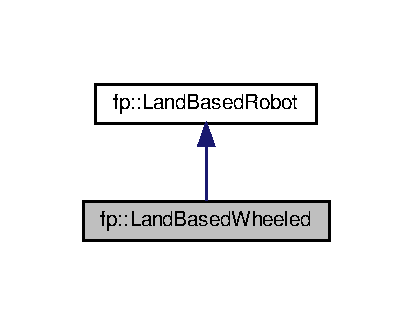
\includegraphics[width=198pt]{classfp_1_1_land_based_wheeled__inherit__graph}
\end{center}
\end{figure}


Collaboration diagram for fp\+:\+:Land\+Based\+Wheeled\+:\nopagebreak
\begin{figure}[H]
\begin{center}
\leavevmode
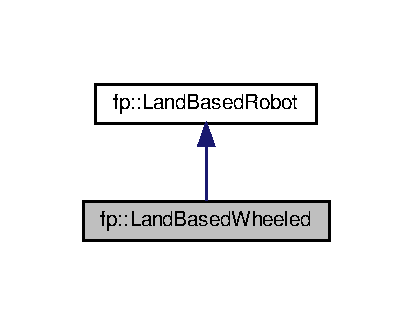
\includegraphics[width=198pt]{classfp_1_1_land_based_wheeled__coll__graph}
\end{center}
\end{figure}
\subsection*{Public Member Functions}
\begin{DoxyCompactItemize}
\item 
\hyperlink{classfp_1_1_land_based_wheeled_a0fe67f1df86ad377e0ef9d64a64f9416}{Land\+Based\+Wheeled} (std\+::string name=\char`\"{}wheeled\char`\"{}, int x=1, int y=4, char direction=\textquotesingle{}N\textquotesingle{})
\item 
virtual char \hyperlink{classfp_1_1_land_based_wheeled_adaafaceb388374ffb9cec28301665492}{Get\+Direction} () override
\item 
virtual void \hyperlink{classfp_1_1_land_based_wheeled_a9c6a668ce9233468141516c8ea678593}{Move\+Forward} (int x, int y) override
\item 
void \hyperlink{classfp_1_1_land_based_wheeled_ad7e32884e0747b347d5d74db171c2854}{Turn\+Left} (int x, int y) override
\item 
void \hyperlink{classfp_1_1_land_based_wheeled_a759f28e9ca00e77cc0e2f2ce2f524811}{Turn\+Right} (int x, int y) override
\item 
virtual \hyperlink{classfp_1_1_land_based_wheeled_a932593879ef390bf1b019ddb3cfa604d}{$\sim$\+Land\+Based\+Wheeled} ()
\end{DoxyCompactItemize}
\subsection*{Public Attributes}
\begin{DoxyCompactItemize}
\item 
double \hyperlink{classfp_1_1_land_based_wheeled_aaab6e766362d75c7e52a183256123a36}{speed} = \hyperlink{classfp_1_1_land_based_robot_a44fed3a00505f6679ff8505aebae4505}{Land\+Based\+Robot\+::get\+\_\+speed}()
\item 
double \hyperlink{classfp_1_1_land_based_wheeled_af340cd88db06fdbb837eddedf7ec9c14}{width} = \hyperlink{classfp_1_1_land_based_robot_a523b439167030a7ab1e0e7f6c8d42315}{Land\+Based\+Robot\+::get\+\_\+width}()
\item 
double \hyperlink{classfp_1_1_land_based_wheeled_a99e87d729bfd9bee5924a387a11052e6}{length} = \hyperlink{classfp_1_1_land_based_robot_adb03fbded9a3b0553301bcc0322cb1c1}{Land\+Based\+Robot\+::get\+\_\+length}()
\item 
double \hyperlink{classfp_1_1_land_based_wheeled_ae56bdd84440e468928e4f416394d5dde}{height} = \hyperlink{classfp_1_1_land_based_robot_ac77253c989c417ee26654541c50669d4}{Land\+Based\+Robot\+::get\+\_\+height}()
\item 
double \hyperlink{classfp_1_1_land_based_wheeled_a724d9e2b23926f461d8afea8311707e3}{capacity} = \hyperlink{classfp_1_1_land_based_robot_a24c0f6d395f3dfd6bdbcf5a2a9801de1}{Land\+Based\+Robot\+::get\+\_\+capacity}()
\end{DoxyCompactItemize}
\subsection*{Protected Attributes}
\begin{DoxyCompactItemize}
\item 
const int \hyperlink{classfp_1_1_land_based_wheeled_ac93d4b44f9091f566ec886ddb9972810}{wheel\+\_\+number}
\item 
const std\+::string \hyperlink{classfp_1_1_land_based_wheeled_a72094d60b6dbfa33b6e5cab4a8e5f7c4}{name\+\_\+}
\item 
double \hyperlink{classfp_1_1_land_based_wheeled_a65bfb90a4e7fe10c87f30d276d9db80c}{speed\+\_\+} \{\}
\item 
double \hyperlink{classfp_1_1_land_based_wheeled_ab36bf6c7c4d986d6e88982b224e1ad1a}{width\+\_\+} \{\}
\item 
double \hyperlink{classfp_1_1_land_based_wheeled_addf50162ea822bf0484978cc08afd07a}{length\+\_\+} \{\}
\item 
double \hyperlink{classfp_1_1_land_based_wheeled_a2a5ae9e9307a22c9538f51ab366d7f57}{height\+\_\+} \{\}
\item 
double \hyperlink{classfp_1_1_land_based_wheeled_abf13221333a556a215b951d45568f03a}{capacity\+\_\+} \{\}
\item 
int \hyperlink{classfp_1_1_land_based_wheeled_a575a73a2601f480d2edbc5daa4cc5bf1}{x\+\_\+} \{\}
\item 
int \hyperlink{classfp_1_1_land_based_wheeled_a5b66ada6988a2b8ce6efafa971dfd9c6}{y\+\_\+} \{\}
\item 
char \hyperlink{classfp_1_1_land_based_wheeled_a71bec8ed4710864eb7a9534b3d39e060}{direction\+\_\+} \{\textquotesingle{}N\textquotesingle{}\}
\end{DoxyCompactItemize}


\subsection{Constructor \& Destructor Documentation}
\mbox{\Hypertarget{classfp_1_1_land_based_wheeled_a0fe67f1df86ad377e0ef9d64a64f9416}\label{classfp_1_1_land_based_wheeled_a0fe67f1df86ad377e0ef9d64a64f9416}} 
\index{fp\+::\+Land\+Based\+Wheeled@{fp\+::\+Land\+Based\+Wheeled}!Land\+Based\+Wheeled@{Land\+Based\+Wheeled}}
\index{Land\+Based\+Wheeled@{Land\+Based\+Wheeled}!fp\+::\+Land\+Based\+Wheeled@{fp\+::\+Land\+Based\+Wheeled}}
\subsubsection{\texorpdfstring{Land\+Based\+Wheeled()}{LandBasedWheeled()}}
{\footnotesize\ttfamily fp\+::\+Land\+Based\+Wheeled\+::\+Land\+Based\+Wheeled (\begin{DoxyParamCaption}\item[{std\+::string}]{name = {\ttfamily \char`\"{}wheeled\char`\"{}},  }\item[{int}]{x = {\ttfamily 1},  }\item[{int}]{y = {\ttfamily 4},  }\item[{char}]{direction = {\ttfamily \textquotesingle{}N\textquotesingle{}} }\end{DoxyParamCaption})\hspace{0.3cm}{\ttfamily [inline]}, {\ttfamily [explicit]}}

\hyperlink{classfp_1_1_land_based_wheeled}{Land\+Based\+Wheeled} Constructor 
\begin{DoxyParams}{Parameters}
{\em name} & name of the robot \\
\hline
{\em x} & x coordinate of the robot \\
\hline
{\em y} & y coordinate of the robot \\
\hline
{\em wheels} & number of wheels on the robot \\
\hline
\end{DoxyParams}
\mbox{\Hypertarget{classfp_1_1_land_based_wheeled_a932593879ef390bf1b019ddb3cfa604d}\label{classfp_1_1_land_based_wheeled_a932593879ef390bf1b019ddb3cfa604d}} 
\index{fp\+::\+Land\+Based\+Wheeled@{fp\+::\+Land\+Based\+Wheeled}!````~Land\+Based\+Wheeled@{$\sim$\+Land\+Based\+Wheeled}}
\index{````~Land\+Based\+Wheeled@{$\sim$\+Land\+Based\+Wheeled}!fp\+::\+Land\+Based\+Wheeled@{fp\+::\+Land\+Based\+Wheeled}}
\subsubsection{\texorpdfstring{$\sim$\+Land\+Based\+Wheeled()}{~LandBasedWheeled()}}
{\footnotesize\ttfamily virtual fp\+::\+Land\+Based\+Wheeled\+::$\sim$\+Land\+Based\+Wheeled (\begin{DoxyParamCaption}{ }\end{DoxyParamCaption})\hspace{0.3cm}{\ttfamily [inline]}, {\ttfamily [virtual]}}



\subsection{Member Function Documentation}
\mbox{\Hypertarget{classfp_1_1_land_based_wheeled_adaafaceb388374ffb9cec28301665492}\label{classfp_1_1_land_based_wheeled_adaafaceb388374ffb9cec28301665492}} 
\index{fp\+::\+Land\+Based\+Wheeled@{fp\+::\+Land\+Based\+Wheeled}!Get\+Direction@{Get\+Direction}}
\index{Get\+Direction@{Get\+Direction}!fp\+::\+Land\+Based\+Wheeled@{fp\+::\+Land\+Based\+Wheeled}}
\subsubsection{\texorpdfstring{Get\+Direction()}{GetDirection()}}
{\footnotesize\ttfamily char fp\+::\+Land\+Based\+Wheeled\+::\+Get\+Direction (\begin{DoxyParamCaption}{ }\end{DoxyParamCaption})\hspace{0.3cm}{\ttfamily [override]}, {\ttfamily [virtual]}}

Virtual Get\+Direction Method Get the direction of the robot in the maze 
\begin{DoxyParams}{Parameters}
{\em x} & x coordinate of the robot \\
\hline
{\em y} & y coordinate of the robot \\
\hline
\end{DoxyParams}


Implements \hyperlink{classfp_1_1_land_based_robot_a50841b6e40d4e92832770d26b427fea2}{fp\+::\+Land\+Based\+Robot}.

\mbox{\Hypertarget{classfp_1_1_land_based_wheeled_a9c6a668ce9233468141516c8ea678593}\label{classfp_1_1_land_based_wheeled_a9c6a668ce9233468141516c8ea678593}} 
\index{fp\+::\+Land\+Based\+Wheeled@{fp\+::\+Land\+Based\+Wheeled}!Move\+Forward@{Move\+Forward}}
\index{Move\+Forward@{Move\+Forward}!fp\+::\+Land\+Based\+Wheeled@{fp\+::\+Land\+Based\+Wheeled}}
\subsubsection{\texorpdfstring{Move\+Forward()}{MoveForward()}}
{\footnotesize\ttfamily void fp\+::\+Land\+Based\+Wheeled\+::\+Move\+Forward (\begin{DoxyParamCaption}\item[{int}]{x,  }\item[{int}]{y }\end{DoxyParamCaption})\hspace{0.3cm}{\ttfamily [override]}, {\ttfamily [virtual]}}

Virtual Move\+Forward Method Moves the robot forward in the maze 
\begin{DoxyParams}{Parameters}
{\em x} & x coordinate of the robot \\
\hline
{\em y} & y coordinate of the robot \\
\hline
\end{DoxyParams}


Implements \hyperlink{classfp_1_1_land_based_robot_a25ed5c4c524e68cc983104a8da57599b}{fp\+::\+Land\+Based\+Robot}.

\mbox{\Hypertarget{classfp_1_1_land_based_wheeled_ad7e32884e0747b347d5d74db171c2854}\label{classfp_1_1_land_based_wheeled_ad7e32884e0747b347d5d74db171c2854}} 
\index{fp\+::\+Land\+Based\+Wheeled@{fp\+::\+Land\+Based\+Wheeled}!Turn\+Left@{Turn\+Left}}
\index{Turn\+Left@{Turn\+Left}!fp\+::\+Land\+Based\+Wheeled@{fp\+::\+Land\+Based\+Wheeled}}
\subsubsection{\texorpdfstring{Turn\+Left()}{TurnLeft()}}
{\footnotesize\ttfamily void fp\+::\+Land\+Based\+Wheeled\+::\+Turn\+Left (\begin{DoxyParamCaption}\item[{int}]{x,  }\item[{int}]{y }\end{DoxyParamCaption})\hspace{0.3cm}{\ttfamily [override]}, {\ttfamily [virtual]}}

Virtual Turn\+Left Method Moves the robot left in the maze 
\begin{DoxyParams}{Parameters}
{\em x} & x coordinate of the robot \\
\hline
{\em y} & y coordinate of the robot \\
\hline
\end{DoxyParams}


Implements \hyperlink{classfp_1_1_land_based_robot_a359e1012e9093475b7a1b0d38e41a118}{fp\+::\+Land\+Based\+Robot}.

\mbox{\Hypertarget{classfp_1_1_land_based_wheeled_a759f28e9ca00e77cc0e2f2ce2f524811}\label{classfp_1_1_land_based_wheeled_a759f28e9ca00e77cc0e2f2ce2f524811}} 
\index{fp\+::\+Land\+Based\+Wheeled@{fp\+::\+Land\+Based\+Wheeled}!Turn\+Right@{Turn\+Right}}
\index{Turn\+Right@{Turn\+Right}!fp\+::\+Land\+Based\+Wheeled@{fp\+::\+Land\+Based\+Wheeled}}
\subsubsection{\texorpdfstring{Turn\+Right()}{TurnRight()}}
{\footnotesize\ttfamily void fp\+::\+Land\+Based\+Wheeled\+::\+Turn\+Right (\begin{DoxyParamCaption}\item[{int}]{x,  }\item[{int}]{y }\end{DoxyParamCaption})\hspace{0.3cm}{\ttfamily [override]}, {\ttfamily [virtual]}}

Virtual Turn\+Right Method Moves the robot right in the maze 
\begin{DoxyParams}{Parameters}
{\em x} & x coordinate of the robot \\
\hline
{\em y} & y coordinate of the robot\+Destructor for \hyperlink{classfp_1_1_land_based_wheeled}{Land\+Based\+Wheeled} \\
\hline
\end{DoxyParams}


Implements \hyperlink{classfp_1_1_land_based_robot_a7360e4084bc5254f72ab0d3612644907}{fp\+::\+Land\+Based\+Robot}.



\subsection{Member Data Documentation}
\mbox{\Hypertarget{classfp_1_1_land_based_wheeled_a724d9e2b23926f461d8afea8311707e3}\label{classfp_1_1_land_based_wheeled_a724d9e2b23926f461d8afea8311707e3}} 
\index{fp\+::\+Land\+Based\+Wheeled@{fp\+::\+Land\+Based\+Wheeled}!capacity@{capacity}}
\index{capacity@{capacity}!fp\+::\+Land\+Based\+Wheeled@{fp\+::\+Land\+Based\+Wheeled}}
\subsubsection{\texorpdfstring{capacity}{capacity}}
{\footnotesize\ttfamily double fp\+::\+Land\+Based\+Wheeled\+::capacity = \hyperlink{classfp_1_1_land_based_robot_a24c0f6d395f3dfd6bdbcf5a2a9801de1}{Land\+Based\+Robot\+::get\+\_\+capacity}()}

\mbox{\Hypertarget{classfp_1_1_land_based_wheeled_abf13221333a556a215b951d45568f03a}\label{classfp_1_1_land_based_wheeled_abf13221333a556a215b951d45568f03a}} 
\index{fp\+::\+Land\+Based\+Wheeled@{fp\+::\+Land\+Based\+Wheeled}!capacity\+\_\+@{capacity\+\_\+}}
\index{capacity\+\_\+@{capacity\+\_\+}!fp\+::\+Land\+Based\+Wheeled@{fp\+::\+Land\+Based\+Wheeled}}
\subsubsection{\texorpdfstring{capacity\+\_\+}{capacity\_}}
{\footnotesize\ttfamily double fp\+::\+Land\+Based\+Wheeled\+::capacity\+\_\+ \{\}\hspace{0.3cm}{\ttfamily [protected]}}

Height of the base of the robot \mbox{\Hypertarget{classfp_1_1_land_based_wheeled_a71bec8ed4710864eb7a9534b3d39e060}\label{classfp_1_1_land_based_wheeled_a71bec8ed4710864eb7a9534b3d39e060}} 
\index{fp\+::\+Land\+Based\+Wheeled@{fp\+::\+Land\+Based\+Wheeled}!direction\+\_\+@{direction\+\_\+}}
\index{direction\+\_\+@{direction\+\_\+}!fp\+::\+Land\+Based\+Wheeled@{fp\+::\+Land\+Based\+Wheeled}}
\subsubsection{\texorpdfstring{direction\+\_\+}{direction\_}}
{\footnotesize\ttfamily char fp\+::\+Land\+Based\+Wheeled\+::direction\+\_\+ \{\textquotesingle{}N\textquotesingle{}\}\hspace{0.3cm}{\ttfamily [protected]}}

Direction that the robot is facing in the maze \mbox{\Hypertarget{classfp_1_1_land_based_wheeled_ae56bdd84440e468928e4f416394d5dde}\label{classfp_1_1_land_based_wheeled_ae56bdd84440e468928e4f416394d5dde}} 
\index{fp\+::\+Land\+Based\+Wheeled@{fp\+::\+Land\+Based\+Wheeled}!height@{height}}
\index{height@{height}!fp\+::\+Land\+Based\+Wheeled@{fp\+::\+Land\+Based\+Wheeled}}
\subsubsection{\texorpdfstring{height}{height}}
{\footnotesize\ttfamily double fp\+::\+Land\+Based\+Wheeled\+::height = \hyperlink{classfp_1_1_land_based_robot_ac77253c989c417ee26654541c50669d4}{Land\+Based\+Robot\+::get\+\_\+height}()}

\mbox{\Hypertarget{classfp_1_1_land_based_wheeled_a2a5ae9e9307a22c9538f51ab366d7f57}\label{classfp_1_1_land_based_wheeled_a2a5ae9e9307a22c9538f51ab366d7f57}} 
\index{fp\+::\+Land\+Based\+Wheeled@{fp\+::\+Land\+Based\+Wheeled}!height\+\_\+@{height\+\_\+}}
\index{height\+\_\+@{height\+\_\+}!fp\+::\+Land\+Based\+Wheeled@{fp\+::\+Land\+Based\+Wheeled}}
\subsubsection{\texorpdfstring{height\+\_\+}{height\_}}
{\footnotesize\ttfamily double fp\+::\+Land\+Based\+Wheeled\+::height\+\_\+ \{\}\hspace{0.3cm}{\ttfamily [protected]}}

Height of the base of the robot \mbox{\Hypertarget{classfp_1_1_land_based_wheeled_a99e87d729bfd9bee5924a387a11052e6}\label{classfp_1_1_land_based_wheeled_a99e87d729bfd9bee5924a387a11052e6}} 
\index{fp\+::\+Land\+Based\+Wheeled@{fp\+::\+Land\+Based\+Wheeled}!length@{length}}
\index{length@{length}!fp\+::\+Land\+Based\+Wheeled@{fp\+::\+Land\+Based\+Wheeled}}
\subsubsection{\texorpdfstring{length}{length}}
{\footnotesize\ttfamily double fp\+::\+Land\+Based\+Wheeled\+::length = \hyperlink{classfp_1_1_land_based_robot_adb03fbded9a3b0553301bcc0322cb1c1}{Land\+Based\+Robot\+::get\+\_\+length}()}

\mbox{\Hypertarget{classfp_1_1_land_based_wheeled_addf50162ea822bf0484978cc08afd07a}\label{classfp_1_1_land_based_wheeled_addf50162ea822bf0484978cc08afd07a}} 
\index{fp\+::\+Land\+Based\+Wheeled@{fp\+::\+Land\+Based\+Wheeled}!length\+\_\+@{length\+\_\+}}
\index{length\+\_\+@{length\+\_\+}!fp\+::\+Land\+Based\+Wheeled@{fp\+::\+Land\+Based\+Wheeled}}
\subsubsection{\texorpdfstring{length\+\_\+}{length\_}}
{\footnotesize\ttfamily double fp\+::\+Land\+Based\+Wheeled\+::length\+\_\+ \{\}\hspace{0.3cm}{\ttfamily [protected]}}

Width of the base of the robot \mbox{\Hypertarget{classfp_1_1_land_based_wheeled_a72094d60b6dbfa33b6e5cab4a8e5f7c4}\label{classfp_1_1_land_based_wheeled_a72094d60b6dbfa33b6e5cab4a8e5f7c4}} 
\index{fp\+::\+Land\+Based\+Wheeled@{fp\+::\+Land\+Based\+Wheeled}!name\+\_\+@{name\+\_\+}}
\index{name\+\_\+@{name\+\_\+}!fp\+::\+Land\+Based\+Wheeled@{fp\+::\+Land\+Based\+Wheeled}}
\subsubsection{\texorpdfstring{name\+\_\+}{name\_}}
{\footnotesize\ttfamily const std\+::string fp\+::\+Land\+Based\+Wheeled\+::name\+\_\+\hspace{0.3cm}{\ttfamily [protected]}}

Name of the robot \mbox{\Hypertarget{classfp_1_1_land_based_wheeled_aaab6e766362d75c7e52a183256123a36}\label{classfp_1_1_land_based_wheeled_aaab6e766362d75c7e52a183256123a36}} 
\index{fp\+::\+Land\+Based\+Wheeled@{fp\+::\+Land\+Based\+Wheeled}!speed@{speed}}
\index{speed@{speed}!fp\+::\+Land\+Based\+Wheeled@{fp\+::\+Land\+Based\+Wheeled}}
\subsubsection{\texorpdfstring{speed}{speed}}
{\footnotesize\ttfamily double fp\+::\+Land\+Based\+Wheeled\+::speed = \hyperlink{classfp_1_1_land_based_robot_a44fed3a00505f6679ff8505aebae4505}{Land\+Based\+Robot\+::get\+\_\+speed}()}

The following are accessors to get the required derived attributes from the base class (\hyperlink{classfp_1_1_land_based_robot}{Land\+Based\+Robot}) \mbox{\Hypertarget{classfp_1_1_land_based_wheeled_a65bfb90a4e7fe10c87f30d276d9db80c}\label{classfp_1_1_land_based_wheeled_a65bfb90a4e7fe10c87f30d276d9db80c}} 
\index{fp\+::\+Land\+Based\+Wheeled@{fp\+::\+Land\+Based\+Wheeled}!speed\+\_\+@{speed\+\_\+}}
\index{speed\+\_\+@{speed\+\_\+}!fp\+::\+Land\+Based\+Wheeled@{fp\+::\+Land\+Based\+Wheeled}}
\subsubsection{\texorpdfstring{speed\+\_\+}{speed\_}}
{\footnotesize\ttfamily double fp\+::\+Land\+Based\+Wheeled\+::speed\+\_\+ \{\}\hspace{0.3cm}{\ttfamily [protected]}}

Driving speed of the robot \mbox{\Hypertarget{classfp_1_1_land_based_wheeled_ac93d4b44f9091f566ec886ddb9972810}\label{classfp_1_1_land_based_wheeled_ac93d4b44f9091f566ec886ddb9972810}} 
\index{fp\+::\+Land\+Based\+Wheeled@{fp\+::\+Land\+Based\+Wheeled}!wheel\+\_\+number@{wheel\+\_\+number}}
\index{wheel\+\_\+number@{wheel\+\_\+number}!fp\+::\+Land\+Based\+Wheeled@{fp\+::\+Land\+Based\+Wheeled}}
\subsubsection{\texorpdfstring{wheel\+\_\+number}{wheel\_number}}
{\footnotesize\ttfamily const int fp\+::\+Land\+Based\+Wheeled\+::wheel\+\_\+number\hspace{0.3cm}{\ttfamily [protected]}}

Number of wheels mounted on the robot \mbox{\Hypertarget{classfp_1_1_land_based_wheeled_af340cd88db06fdbb837eddedf7ec9c14}\label{classfp_1_1_land_based_wheeled_af340cd88db06fdbb837eddedf7ec9c14}} 
\index{fp\+::\+Land\+Based\+Wheeled@{fp\+::\+Land\+Based\+Wheeled}!width@{width}}
\index{width@{width}!fp\+::\+Land\+Based\+Wheeled@{fp\+::\+Land\+Based\+Wheeled}}
\subsubsection{\texorpdfstring{width}{width}}
{\footnotesize\ttfamily double fp\+::\+Land\+Based\+Wheeled\+::width = \hyperlink{classfp_1_1_land_based_robot_a523b439167030a7ab1e0e7f6c8d42315}{Land\+Based\+Robot\+::get\+\_\+width}()}

\mbox{\Hypertarget{classfp_1_1_land_based_wheeled_ab36bf6c7c4d986d6e88982b224e1ad1a}\label{classfp_1_1_land_based_wheeled_ab36bf6c7c4d986d6e88982b224e1ad1a}} 
\index{fp\+::\+Land\+Based\+Wheeled@{fp\+::\+Land\+Based\+Wheeled}!width\+\_\+@{width\+\_\+}}
\index{width\+\_\+@{width\+\_\+}!fp\+::\+Land\+Based\+Wheeled@{fp\+::\+Land\+Based\+Wheeled}}
\subsubsection{\texorpdfstring{width\+\_\+}{width\_}}
{\footnotesize\ttfamily double fp\+::\+Land\+Based\+Wheeled\+::width\+\_\+ \{\}\hspace{0.3cm}{\ttfamily [protected]}}

Width of the base of the robot \mbox{\Hypertarget{classfp_1_1_land_based_wheeled_a575a73a2601f480d2edbc5daa4cc5bf1}\label{classfp_1_1_land_based_wheeled_a575a73a2601f480d2edbc5daa4cc5bf1}} 
\index{fp\+::\+Land\+Based\+Wheeled@{fp\+::\+Land\+Based\+Wheeled}!x\+\_\+@{x\+\_\+}}
\index{x\+\_\+@{x\+\_\+}!fp\+::\+Land\+Based\+Wheeled@{fp\+::\+Land\+Based\+Wheeled}}
\subsubsection{\texorpdfstring{x\+\_\+}{x\_}}
{\footnotesize\ttfamily int fp\+::\+Land\+Based\+Wheeled\+::x\+\_\+ \{\}\hspace{0.3cm}{\ttfamily [protected]}}

x coordinate of the robot \mbox{\Hypertarget{classfp_1_1_land_based_wheeled_a5b66ada6988a2b8ce6efafa971dfd9c6}\label{classfp_1_1_land_based_wheeled_a5b66ada6988a2b8ce6efafa971dfd9c6}} 
\index{fp\+::\+Land\+Based\+Wheeled@{fp\+::\+Land\+Based\+Wheeled}!y\+\_\+@{y\+\_\+}}
\index{y\+\_\+@{y\+\_\+}!fp\+::\+Land\+Based\+Wheeled@{fp\+::\+Land\+Based\+Wheeled}}
\subsubsection{\texorpdfstring{y\+\_\+}{y\_}}
{\footnotesize\ttfamily int fp\+::\+Land\+Based\+Wheeled\+::y\+\_\+ \{\}\hspace{0.3cm}{\ttfamily [protected]}}

y coordinate of the robot 

The documentation for this class was generated from the following files\+:\begin{DoxyCompactItemize}
\item 
/home/diane/\+One\+Drive/\+Fall 2020/\+E\+N\+P\+M809\+Y Intro Robot Programming/\+Homework/\+Final-\/\+Project-\/\+Group3/src/\+Land\+Based\+Wheeled/\hyperlink{landbasedwheeled_8h}{landbasedwheeled.\+h}\item 
/home/diane/\+One\+Drive/\+Fall 2020/\+E\+N\+P\+M809\+Y Intro Robot Programming/\+Homework/\+Final-\/\+Project-\/\+Group3/src/\+Land\+Based\+Wheeled/\hyperlink{landbasedwheeled_8cpp}{landbasedwheeled.\+cpp}\end{DoxyCompactItemize}

\hypertarget{classfp_1_1_maze}{}\section{fp\+:\+:Maze Class Reference}
\label{classfp_1_1_maze}\index{fp\+::\+Maze@{fp\+::\+Maze}}


{\ttfamily \#include $<$Maze.\+h$>$}

\subsection*{Public Member Functions}
\begin{DoxyCompactItemize}
\item 
\hyperlink{classfp_1_1_maze_af090b97595ed34cad9f7c8de9e79a127}{Maze} ()
\item 
void \hyperlink{classfp_1_1_maze_af1ffa713840a40bdcedb99e79ea5bde3}{Set\+Center} ()
\item 
void \hyperlink{classfp_1_1_maze_ace62554f667bd404e059bb61166e44f0}{Set\+Path\+Color} (std\+::array$<$ int, 2 $>$ start\+\_\+node)
\end{DoxyCompactItemize}
\subsection*{Static Public Member Functions}
\begin{DoxyCompactItemize}
\item 
static void \hyperlink{classfp_1_1_maze_a689d998d05f671c2644804ee912c5e79}{Set\+Perimeter\+Walls} ()
\end{DoxyCompactItemize}
\subsection*{Public Attributes}
\begin{DoxyCompactItemize}
\item 
int \hyperlink{classfp_1_1_maze_a8610720d37ec84d7b2192b13334ea525}{maze\+\_\+arr} \mbox{[}\hyperlink{classfp_1_1_maze_ae976c87b67bf82c41ede75a19ac28c2c}{M\+A\+Z\+E\+\_\+\+W\+I\+D\+TH}\mbox{]}\mbox{[}\hyperlink{classfp_1_1_maze_a3cee2050b4d60bceacc9307e7016b931}{M\+A\+Z\+E\+\_\+\+H\+E\+I\+G\+HT}\mbox{]}
\item 
std\+::array$<$ std\+::array$<$ bool, 16 $>$, 2 $>$ \hyperlink{classfp_1_1_maze_a7a16c86454b8898a4ba6a913cbfcb67e}{north\+\_\+}
\item 
std\+::array$<$ std\+::array$<$ bool, 16 $>$, 2 $>$ \hyperlink{classfp_1_1_maze_ab494935167a2bf7f358b72e6c032eef8}{south\+\_\+}
\item 
std\+::array$<$ std\+::array$<$ bool, 16 $>$, 2 $>$ \hyperlink{classfp_1_1_maze_ac1d6b5fc763eff421af708aa39f2141a}{east\+\_\+}
\item 
std\+::array$<$ std\+::array$<$ bool, 16 $>$, 2 $>$ \hyperlink{classfp_1_1_maze_afc8b97457d6f4ff69ed812741982c298}{west\+\_\+}
\item 
bool \hyperlink{classfp_1_1_maze_abdf504125bc0cd3ea18ba17b0887a5a2}{Unsolvable}
\end{DoxyCompactItemize}
\subsection*{Static Public Attributes}
\begin{DoxyCompactItemize}
\item 
static const int \hyperlink{classfp_1_1_maze_ae976c87b67bf82c41ede75a19ac28c2c}{M\+A\+Z\+E\+\_\+\+W\+I\+D\+TH} = 16
\item 
static const int \hyperlink{classfp_1_1_maze_a3cee2050b4d60bceacc9307e7016b931}{M\+A\+Z\+E\+\_\+\+H\+E\+I\+G\+HT} = 16
\end{DoxyCompactItemize}


\subsection{Constructor \& Destructor Documentation}
\mbox{\Hypertarget{classfp_1_1_maze_af090b97595ed34cad9f7c8de9e79a127}\label{classfp_1_1_maze_af090b97595ed34cad9f7c8de9e79a127}} 
\index{fp\+::\+Maze@{fp\+::\+Maze}!Maze@{Maze}}
\index{Maze@{Maze}!fp\+::\+Maze@{fp\+::\+Maze}}
\subsubsection{\texorpdfstring{Maze()}{Maze()}}
{\footnotesize\ttfamily fp\+::\+Maze\+::\+Maze (\begin{DoxyParamCaption}{ }\end{DoxyParamCaption})\hspace{0.3cm}{\ttfamily [inline]}}

Constructor for maze 

\subsection{Member Function Documentation}
\mbox{\Hypertarget{classfp_1_1_maze_af1ffa713840a40bdcedb99e79ea5bde3}\label{classfp_1_1_maze_af1ffa713840a40bdcedb99e79ea5bde3}} 
\index{fp\+::\+Maze@{fp\+::\+Maze}!Set\+Center@{Set\+Center}}
\index{Set\+Center@{Set\+Center}!fp\+::\+Maze@{fp\+::\+Maze}}
\subsubsection{\texorpdfstring{Set\+Center()}{SetCenter()}}
{\footnotesize\ttfamily void fp\+::\+Maze\+::\+Set\+Center (\begin{DoxyParamCaption}{ }\end{DoxyParamCaption})}

Initialize center of the maze by setting the color and text of the 4 center tiles \mbox{\Hypertarget{classfp_1_1_maze_ace62554f667bd404e059bb61166e44f0}\label{classfp_1_1_maze_ace62554f667bd404e059bb61166e44f0}} 
\index{fp\+::\+Maze@{fp\+::\+Maze}!Set\+Path\+Color@{Set\+Path\+Color}}
\index{Set\+Path\+Color@{Set\+Path\+Color}!fp\+::\+Maze@{fp\+::\+Maze}}
\subsubsection{\texorpdfstring{Set\+Path\+Color()}{SetPathColor()}}
{\footnotesize\ttfamily void fp\+::\+Maze\+::\+Set\+Path\+Color (\begin{DoxyParamCaption}\item[{std\+::array$<$ int, 2 $>$}]{start\+\_\+node }\end{DoxyParamCaption})}

Sets the path color as the robot travels 
\begin{DoxyParams}{Parameters}
{\em start\+\_\+node} & starting position of the robot \\
\hline
\end{DoxyParams}
\mbox{\Hypertarget{classfp_1_1_maze_a689d998d05f671c2644804ee912c5e79}\label{classfp_1_1_maze_a689d998d05f671c2644804ee912c5e79}} 
\index{fp\+::\+Maze@{fp\+::\+Maze}!Set\+Perimeter\+Walls@{Set\+Perimeter\+Walls}}
\index{Set\+Perimeter\+Walls@{Set\+Perimeter\+Walls}!fp\+::\+Maze@{fp\+::\+Maze}}
\subsubsection{\texorpdfstring{Set\+Perimeter\+Walls()}{SetPerimeterWalls()}}
{\footnotesize\ttfamily void fp\+::\+Maze\+::\+Set\+Perimeter\+Walls (\begin{DoxyParamCaption}{ }\end{DoxyParamCaption})\hspace{0.3cm}{\ttfamily [static]}}

Set the perimeter walls 

\subsection{Member Data Documentation}
\mbox{\Hypertarget{classfp_1_1_maze_ac1d6b5fc763eff421af708aa39f2141a}\label{classfp_1_1_maze_ac1d6b5fc763eff421af708aa39f2141a}} 
\index{fp\+::\+Maze@{fp\+::\+Maze}!east\+\_\+@{east\+\_\+}}
\index{east\+\_\+@{east\+\_\+}!fp\+::\+Maze@{fp\+::\+Maze}}
\subsubsection{\texorpdfstring{east\+\_\+}{east\_}}
{\footnotesize\ttfamily std\+::array$<$std\+::array$<$bool, 16$>$, 2$>$ fp\+::\+Maze\+::east\+\_\+}

\mbox{\Hypertarget{classfp_1_1_maze_a8610720d37ec84d7b2192b13334ea525}\label{classfp_1_1_maze_a8610720d37ec84d7b2192b13334ea525}} 
\index{fp\+::\+Maze@{fp\+::\+Maze}!maze\+\_\+arr@{maze\+\_\+arr}}
\index{maze\+\_\+arr@{maze\+\_\+arr}!fp\+::\+Maze@{fp\+::\+Maze}}
\subsubsection{\texorpdfstring{maze\+\_\+arr}{maze\_arr}}
{\footnotesize\ttfamily int fp\+::\+Maze\+::maze\+\_\+arr\mbox{[}\hyperlink{classfp_1_1_maze_ae976c87b67bf82c41ede75a19ac28c2c}{M\+A\+Z\+E\+\_\+\+W\+I\+D\+TH}\mbox{]}\mbox{[}\hyperlink{classfp_1_1_maze_a3cee2050b4d60bceacc9307e7016b931}{M\+A\+Z\+E\+\_\+\+H\+E\+I\+G\+HT}\mbox{]}}

Define the maze as 16x16 2D array \mbox{\Hypertarget{classfp_1_1_maze_a3cee2050b4d60bceacc9307e7016b931}\label{classfp_1_1_maze_a3cee2050b4d60bceacc9307e7016b931}} 
\index{fp\+::\+Maze@{fp\+::\+Maze}!M\+A\+Z\+E\+\_\+\+H\+E\+I\+G\+HT@{M\+A\+Z\+E\+\_\+\+H\+E\+I\+G\+HT}}
\index{M\+A\+Z\+E\+\_\+\+H\+E\+I\+G\+HT@{M\+A\+Z\+E\+\_\+\+H\+E\+I\+G\+HT}!fp\+::\+Maze@{fp\+::\+Maze}}
\subsubsection{\texorpdfstring{M\+A\+Z\+E\+\_\+\+H\+E\+I\+G\+HT}{MAZE\_HEIGHT}}
{\footnotesize\ttfamily const int fp\+::\+Maze\+::\+M\+A\+Z\+E\+\_\+\+H\+E\+I\+G\+HT = 16\hspace{0.3cm}{\ttfamily [static]}}

Define the maze height \mbox{\Hypertarget{classfp_1_1_maze_ae976c87b67bf82c41ede75a19ac28c2c}\label{classfp_1_1_maze_ae976c87b67bf82c41ede75a19ac28c2c}} 
\index{fp\+::\+Maze@{fp\+::\+Maze}!M\+A\+Z\+E\+\_\+\+W\+I\+D\+TH@{M\+A\+Z\+E\+\_\+\+W\+I\+D\+TH}}
\index{M\+A\+Z\+E\+\_\+\+W\+I\+D\+TH@{M\+A\+Z\+E\+\_\+\+W\+I\+D\+TH}!fp\+::\+Maze@{fp\+::\+Maze}}
\subsubsection{\texorpdfstring{M\+A\+Z\+E\+\_\+\+W\+I\+D\+TH}{MAZE\_WIDTH}}
{\footnotesize\ttfamily const int fp\+::\+Maze\+::\+M\+A\+Z\+E\+\_\+\+W\+I\+D\+TH = 16\hspace{0.3cm}{\ttfamily [static]}}

Define the maze width \mbox{\Hypertarget{classfp_1_1_maze_a7a16c86454b8898a4ba6a913cbfcb67e}\label{classfp_1_1_maze_a7a16c86454b8898a4ba6a913cbfcb67e}} 
\index{fp\+::\+Maze@{fp\+::\+Maze}!north\+\_\+@{north\+\_\+}}
\index{north\+\_\+@{north\+\_\+}!fp\+::\+Maze@{fp\+::\+Maze}}
\subsubsection{\texorpdfstring{north\+\_\+}{north\_}}
{\footnotesize\ttfamily std\+::array$<$std\+::array$<$bool, 16$>$, 2$>$ fp\+::\+Maze\+::north\+\_\+}

\mbox{\Hypertarget{classfp_1_1_maze_ab494935167a2bf7f358b72e6c032eef8}\label{classfp_1_1_maze_ab494935167a2bf7f358b72e6c032eef8}} 
\index{fp\+::\+Maze@{fp\+::\+Maze}!south\+\_\+@{south\+\_\+}}
\index{south\+\_\+@{south\+\_\+}!fp\+::\+Maze@{fp\+::\+Maze}}
\subsubsection{\texorpdfstring{south\+\_\+}{south\_}}
{\footnotesize\ttfamily std\+::array$<$std\+::array$<$bool, 16$>$, 2$>$ fp\+::\+Maze\+::south\+\_\+}

\mbox{\Hypertarget{classfp_1_1_maze_abdf504125bc0cd3ea18ba17b0887a5a2}\label{classfp_1_1_maze_abdf504125bc0cd3ea18ba17b0887a5a2}} 
\index{fp\+::\+Maze@{fp\+::\+Maze}!Unsolvable@{Unsolvable}}
\index{Unsolvable@{Unsolvable}!fp\+::\+Maze@{fp\+::\+Maze}}
\subsubsection{\texorpdfstring{Unsolvable}{Unsolvable}}
{\footnotesize\ttfamily bool fp\+::\+Maze\+::\+Unsolvable}

\mbox{\Hypertarget{classfp_1_1_maze_afc8b97457d6f4ff69ed812741982c298}\label{classfp_1_1_maze_afc8b97457d6f4ff69ed812741982c298}} 
\index{fp\+::\+Maze@{fp\+::\+Maze}!west\+\_\+@{west\+\_\+}}
\index{west\+\_\+@{west\+\_\+}!fp\+::\+Maze@{fp\+::\+Maze}}
\subsubsection{\texorpdfstring{west\+\_\+}{west\_}}
{\footnotesize\ttfamily std\+::array$<$std\+::array$<$bool, 16$>$, 2$>$ fp\+::\+Maze\+::west\+\_\+}



The documentation for this class was generated from the following files\+:\begin{DoxyCompactItemize}
\item 
/home/diane/\+One\+Drive/\+Fall 2020/\+E\+N\+P\+M809\+Y Intro Robot Programming/\+Homework/\+Final-\/\+Project-\/\+Group3/src/\+Maze/\hyperlink{_maze_8h}{Maze.\+h}\item 
/home/diane/\+One\+Drive/\+Fall 2020/\+E\+N\+P\+M809\+Y Intro Robot Programming/\+Homework/\+Final-\/\+Project-\/\+Group3/src/\+Maze/\hyperlink{_maze_8cpp}{Maze.\+cpp}\end{DoxyCompactItemize}

\hypertarget{structfp_1_1_algorithm_1_1_position}{}\section{fp\+:\+:Algorithm\+:\+:Position Struct Reference}
\label{structfp_1_1_algorithm_1_1_position}\index{fp\+::\+Algorithm\+::\+Position@{fp\+::\+Algorithm\+::\+Position}}


{\ttfamily \#include $<$Algorithm.\+h$>$}

\subsection*{Public Attributes}
\begin{DoxyCompactItemize}
\item 
int \hyperlink{structfp_1_1_algorithm_1_1_position_a3ff5edbcb349dc2f7fcc17b9b7d646f8}{x} \{0\}
\item 
int \hyperlink{structfp_1_1_algorithm_1_1_position_a78a81d6698d3fb3479a433d389fac322}{y} \{0\}
\end{DoxyCompactItemize}


\subsection{Detailed Description}
\hyperlink{structfp_1_1_algorithm_1_1_position}{Position} structure for the x and y coordinate of the robot 

\subsection{Member Data Documentation}
\mbox{\Hypertarget{structfp_1_1_algorithm_1_1_position_a3ff5edbcb349dc2f7fcc17b9b7d646f8}\label{structfp_1_1_algorithm_1_1_position_a3ff5edbcb349dc2f7fcc17b9b7d646f8}} 
\index{fp\+::\+Algorithm\+::\+Position@{fp\+::\+Algorithm\+::\+Position}!x@{x}}
\index{x@{x}!fp\+::\+Algorithm\+::\+Position@{fp\+::\+Algorithm\+::\+Position}}
\subsubsection{\texorpdfstring{x}{x}}
{\footnotesize\ttfamily int fp\+::\+Algorithm\+::\+Position\+::x \{0\}}

\mbox{\Hypertarget{structfp_1_1_algorithm_1_1_position_a78a81d6698d3fb3479a433d389fac322}\label{structfp_1_1_algorithm_1_1_position_a78a81d6698d3fb3479a433d389fac322}} 
\index{fp\+::\+Algorithm\+::\+Position@{fp\+::\+Algorithm\+::\+Position}!y@{y}}
\index{y@{y}!fp\+::\+Algorithm\+::\+Position@{fp\+::\+Algorithm\+::\+Position}}
\subsubsection{\texorpdfstring{y}{y}}
{\footnotesize\ttfamily int fp\+::\+Algorithm\+::\+Position\+::y \{0\}}



The documentation for this struct was generated from the following file\+:\begin{DoxyCompactItemize}
\item 
/home/diane/\+One\+Drive/\+Fall 2020/\+E\+N\+P\+M809\+Y Intro Robot Programming/\+Homework/\+Final-\/\+Project-\/\+Group3/src/\+Algorithm/\hyperlink{_algorithm_8h}{Algorithm.\+h}\end{DoxyCompactItemize}

\chapter{File Documentation}
\hypertarget{main_8cpp}{}\section{main.\+cpp File Reference}
\label{main_8cpp}\index{main.\+cpp@{main.\+cpp}}
{\ttfamily \#include $<$iostream$>$}\newline
Include dependency graph for main.\+cpp\+:\nopagebreak
\begin{figure}[H]
\begin{center}
\leavevmode
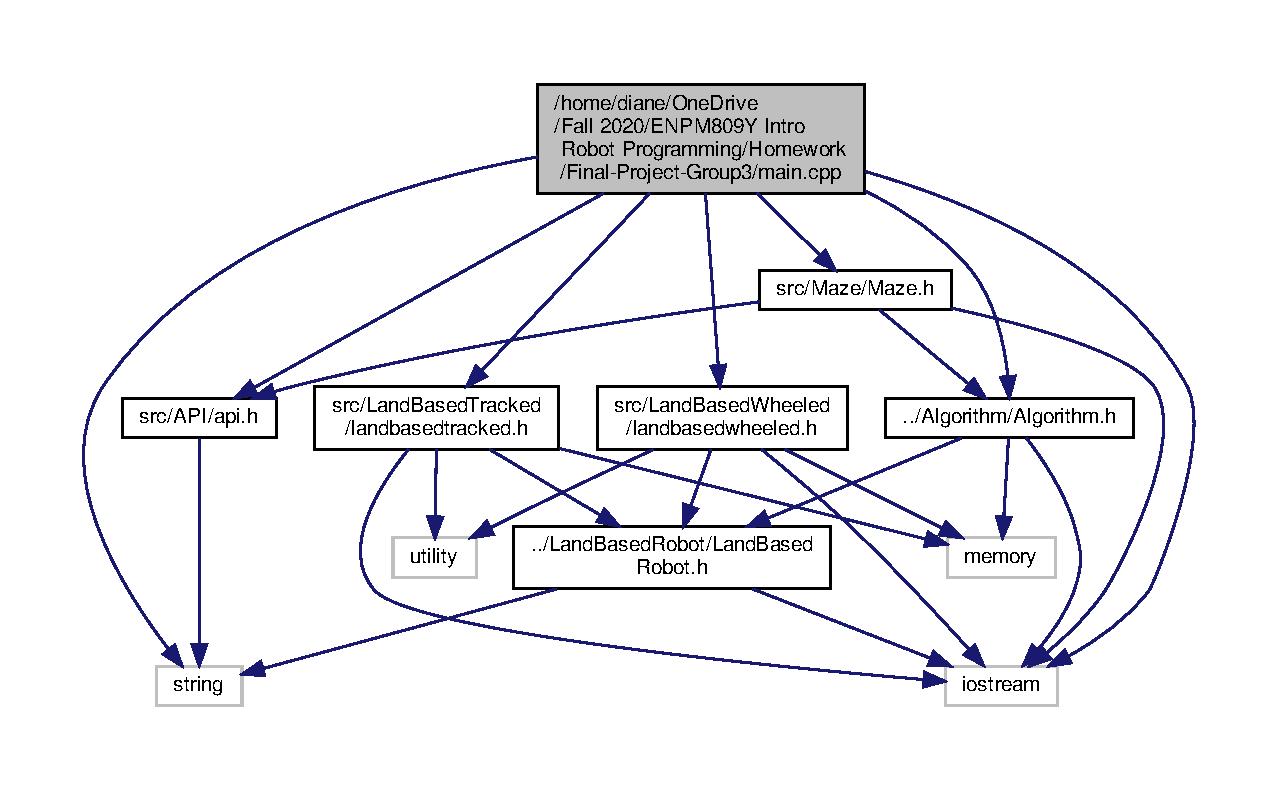
\includegraphics[width=136pt]{main_8cpp__incl}
\end{center}
\end{figure}
\subsection*{Macros}
\begin{DoxyCompactItemize}
\item 
\#define \hyperlink{main_8cpp_a3cfd3aa62338d12609f6d65bce97e9cd}{R\+O\+WS}~6
\begin{DoxyCompactList}\small\item\em Number of Rows for the Maze. \end{DoxyCompactList}\item 
\#define \hyperlink{main_8cpp_ab59ad2ee1a48b83c2eef1f019ed8cc48}{C\+O\+LS}~8
\begin{DoxyCompactList}\small\item\em Number of Columns for the Maze. \end{DoxyCompactList}\end{DoxyCompactItemize}
\subsection*{Functions}
\begin{DoxyCompactItemize}
\item 
bool \hyperlink{main_8cpp_acfa4bb7c74cebff4cd34982630e27e5a}{Check\+Wall} (char maze\mbox{[}6\mbox{]}\mbox{[}8\mbox{]}, int \&x, int \&y)
\item 
bool \hyperlink{main_8cpp_a15ab7ba904c0f46588d62b302075a8c3}{Check\+Outside} (int \&x, int \&y)
\item 
bool \hyperlink{main_8cpp_aefd146022809df49fb9ba712ecb00ffe}{Back\+Track} (char maze\mbox{[}6\mbox{]}\mbox{[}8\mbox{]}, int \&x, int \&y)
\item 
void \hyperlink{main_8cpp_a41b5491830aa7fa26ded753af127966f}{display\+\_\+maze} (char maze\mbox{[}6\mbox{]}\mbox{[}8\mbox{]})
\item 
bool \hyperlink{main_8cpp_acafe6eccc9f6c953bc9b609f732b2273}{Find\+Path} (char maze\mbox{[}6\mbox{]}\mbox{[}8\mbox{]}, int x, int y)
\item 
int \hyperlink{main_8cpp_ae66f6b31b5ad750f1fe042a706a4e3d4}{main} ()
\end{DoxyCompactItemize}


\subsection{Macro Definition Documentation}
\mbox{\Hypertarget{main_8cpp_ab59ad2ee1a48b83c2eef1f019ed8cc48}\label{main_8cpp_ab59ad2ee1a48b83c2eef1f019ed8cc48}} 
\index{main.\+cpp@{main.\+cpp}!C\+O\+LS@{C\+O\+LS}}
\index{C\+O\+LS@{C\+O\+LS}!main.\+cpp@{main.\+cpp}}
\subsubsection{\texorpdfstring{C\+O\+LS}{COLS}}
{\footnotesize\ttfamily \#define C\+O\+LS~8}



Number of Columns for the Maze. 

\mbox{\Hypertarget{main_8cpp_a3cfd3aa62338d12609f6d65bce97e9cd}\label{main_8cpp_a3cfd3aa62338d12609f6d65bce97e9cd}} 
\index{main.\+cpp@{main.\+cpp}!R\+O\+WS@{R\+O\+WS}}
\index{R\+O\+WS@{R\+O\+WS}!main.\+cpp@{main.\+cpp}}
\subsubsection{\texorpdfstring{R\+O\+WS}{ROWS}}
{\footnotesize\ttfamily \#define R\+O\+WS~6}



Number of Rows for the Maze. 



\subsection{Function Documentation}
\mbox{\Hypertarget{main_8cpp_aefd146022809df49fb9ba712ecb00ffe}\label{main_8cpp_aefd146022809df49fb9ba712ecb00ffe}} 
\index{main.\+cpp@{main.\+cpp}!Back\+Track@{Back\+Track}}
\index{Back\+Track@{Back\+Track}!main.\+cpp@{main.\+cpp}}
\subsubsection{\texorpdfstring{Back\+Track()}{BackTrack()}}
{\footnotesize\ttfamily bool Back\+Track (\begin{DoxyParamCaption}\item[{char}]{maze\mbox{[}6\mbox{]}\mbox{[}8\mbox{]},  }\item[{int \&}]{x,  }\item[{int \&}]{y }\end{DoxyParamCaption})}

Function to backtrack if the coordinate has been visited and there is no path found 
\begin{DoxyParams}{Parameters}
{\em maze} & the 2D array of character for the maze \\
\hline
{\em x} & integer of the x coordinate \\
\hline
{\em y} & integer of the y coordinate \\
\hline
\end{DoxyParams}
\begin{DoxyReturn}{Returns}

\end{DoxyReturn}
\mbox{\Hypertarget{main_8cpp_a15ab7ba904c0f46588d62b302075a8c3}\label{main_8cpp_a15ab7ba904c0f46588d62b302075a8c3}} 
\index{main.\+cpp@{main.\+cpp}!Check\+Outside@{Check\+Outside}}
\index{Check\+Outside@{Check\+Outside}!main.\+cpp@{main.\+cpp}}
\subsubsection{\texorpdfstring{Check\+Outside()}{CheckOutside()}}
{\footnotesize\ttfamily bool Check\+Outside (\begin{DoxyParamCaption}\item[{int \&}]{x,  }\item[{int \&}]{y }\end{DoxyParamCaption})}

Check\+Outside Function\+: Function to check if the desired direction is outside of the maze 
\begin{DoxyParams}{Parameters}
{\em maze} & the 2D array of character for the maze \\
\hline
{\em x} & integer of the x coordinate \\
\hline
{\em y} & integer of the y coordinate \\
\hline
\end{DoxyParams}
\begin{DoxyReturn}{Returns}

\end{DoxyReturn}
\mbox{\Hypertarget{main_8cpp_acfa4bb7c74cebff4cd34982630e27e5a}\label{main_8cpp_acfa4bb7c74cebff4cd34982630e27e5a}} 
\index{main.\+cpp@{main.\+cpp}!Check\+Wall@{Check\+Wall}}
\index{Check\+Wall@{Check\+Wall}!main.\+cpp@{main.\+cpp}}
\subsubsection{\texorpdfstring{Check\+Wall()}{CheckWall()}}
{\footnotesize\ttfamily bool Check\+Wall (\begin{DoxyParamCaption}\item[{char}]{maze\mbox{[}6\mbox{]}\mbox{[}8\mbox{]},  }\item[{int \&}]{x,  }\item[{int \&}]{y }\end{DoxyParamCaption})}

Check\+Wall Function\+: Function to check if there is a wall in the desired direction 
\begin{DoxyParams}{Parameters}
{\em maze} & the 2D array of character for the maze \\
\hline
{\em x} & integer of the x coordinate \\
\hline
{\em y} & integer of the y coordinate \\
\hline
\end{DoxyParams}
\begin{DoxyReturn}{Returns}

\end{DoxyReturn}
\mbox{\Hypertarget{main_8cpp_a41b5491830aa7fa26ded753af127966f}\label{main_8cpp_a41b5491830aa7fa26ded753af127966f}} 
\index{main.\+cpp@{main.\+cpp}!display\+\_\+maze@{display\+\_\+maze}}
\index{display\+\_\+maze@{display\+\_\+maze}!main.\+cpp@{main.\+cpp}}
\subsubsection{\texorpdfstring{display\+\_\+maze()}{display\_maze()}}
{\footnotesize\ttfamily void display\+\_\+maze (\begin{DoxyParamCaption}\item[{char}]{maze\mbox{[}6\mbox{]}\mbox{[}8\mbox{]} }\end{DoxyParamCaption})}

Function to display the maze 
\begin{DoxyParams}{Parameters}
{\em maze} & the 2d array of characters for the maze \\
\hline
\end{DoxyParams}
\mbox{\Hypertarget{main_8cpp_acafe6eccc9f6c953bc9b609f732b2273}\label{main_8cpp_acafe6eccc9f6c953bc9b609f732b2273}} 
\index{main.\+cpp@{main.\+cpp}!Find\+Path@{Find\+Path}}
\index{Find\+Path@{Find\+Path}!main.\+cpp@{main.\+cpp}}
\subsubsection{\texorpdfstring{Find\+Path()}{FindPath()}}
{\footnotesize\ttfamily bool Find\+Path (\begin{DoxyParamCaption}\item[{char}]{maze\mbox{[}6\mbox{]}\mbox{[}8\mbox{]},  }\item[{int}]{x,  }\item[{int}]{y }\end{DoxyParamCaption})}

Find\+Path Function is a recursive function to iterate through the maze by checking North, East, South, and West. It checks if there is a wall at the position or if its outside of the maze, then proceeds by placing a + sign at the position and updates. 
\begin{DoxyParams}{Parameters}
{\em maze} & the 2D array of character for the maze \\
\hline
{\em x} & integer of the x coordinate \\
\hline
{\em y} & integer of the y coordinate \\
\hline
\end{DoxyParams}
\begin{DoxyReturn}{Returns}

\end{DoxyReturn}
If the x, y is at the goal position

If the coordinates is not at the goal position

Declare outside variable

Declare wall variable

Declare backtrack variable

If x, y is outside of the maze or is a wall

Mark path

Checking North

Checking East

Checking South

Checking West

Backtrack by setting the coordinate back to . \mbox{\Hypertarget{main_8cpp_ae66f6b31b5ad750f1fe042a706a4e3d4}\label{main_8cpp_ae66f6b31b5ad750f1fe042a706a4e3d4}} 
\index{main.\+cpp@{main.\+cpp}!main@{main}}
\index{main@{main}!main.\+cpp@{main.\+cpp}}
\subsubsection{\texorpdfstring{main()}{main()}}
{\footnotesize\ttfamily int main (\begin{DoxyParamCaption}{ }\end{DoxyParamCaption})}

Maze array is reversed to print it out with respect to the coordinate system

Initialize the variables for the starting position

Initialize temporary variables s\+\_\+x and s\+\_\+y to save the new input

User Input

While Loop to determine if start and goal position are inside of the maze and not a wall

This if loop checks if the desired starting position is outside of the maze.

set the s array to coordinates x, y

Initialize temporary variables g\+\_\+x and g\+\_\+y to save the new input

This if loop checks if the desired goal position is outside of the maze.

set the g array to coordinates x, y 
\hypertarget{_algorithm_8cpp}{}\section{/home/diane/\+One\+Drive/\+Fall 2020/\+E\+N\+P\+M809Y Intro Robot Programming/\+Homework/\+Final-\/\+Project-\/\+Group3/src/\+Algorithm/\+Algorithm.cpp File Reference}
\label{_algorithm_8cpp}\index{/home/diane/\+One\+Drive/\+Fall 2020/\+E\+N\+P\+M809\+Y Intro Robot Programming/\+Homework/\+Final-\/\+Project-\/\+Group3/src/\+Algorithm/\+Algorithm.\+cpp@{/home/diane/\+One\+Drive/\+Fall 2020/\+E\+N\+P\+M809\+Y Intro Robot Programming/\+Homework/\+Final-\/\+Project-\/\+Group3/src/\+Algorithm/\+Algorithm.\+cpp}}
{\ttfamily \#include \char`\"{}Algorithm.\+h\char`\"{}}\newline
{\ttfamily \#include $<$iostream$>$}\newline
{\ttfamily \#include $<$string$>$}\newline
{\ttfamily \#include \char`\"{}../\+A\+P\+I/api.\+h\char`\"{}}\newline
{\ttfamily \#include \char`\"{}../\+Maze/\+Maze.\+h\char`\"{}}\newline
{\ttfamily \#include \char`\"{}../\+Land\+Based\+Robot/\+Land\+Based\+Robot.\+h\char`\"{}}\newline
Include dependency graph for Algorithm.\+cpp\+:\nopagebreak
\begin{figure}[H]
\begin{center}
\leavevmode
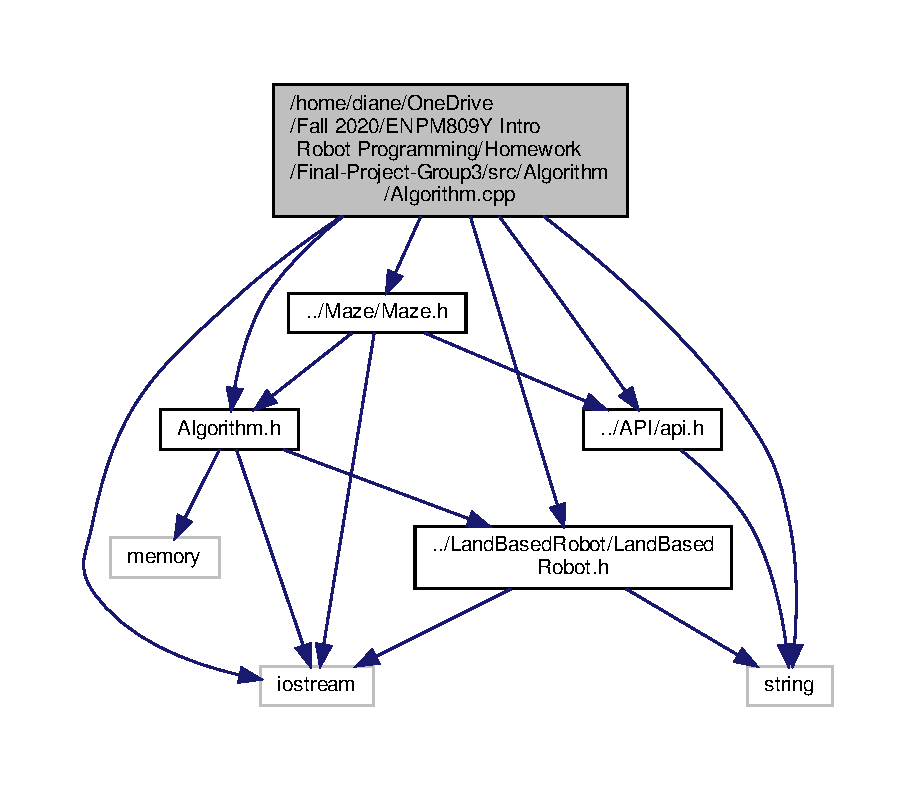
\includegraphics[width=350pt]{_algorithm_8cpp__incl}
\end{center}
\end{figure}

\hypertarget{_algorithm_8h}{}\section{/home/diane/\+One\+Drive/\+Fall 2020/\+E\+N\+P\+M809Y Intro Robot Programming/\+Homework/\+Final-\/\+Project-\/\+Group3/src/\+Algorithm/\+Algorithm.h File Reference}
\label{_algorithm_8h}\index{/home/diane/\+One\+Drive/\+Fall 2020/\+E\+N\+P\+M809\+Y Intro Robot Programming/\+Homework/\+Final-\/\+Project-\/\+Group3/src/\+Algorithm/\+Algorithm.\+h@{/home/diane/\+One\+Drive/\+Fall 2020/\+E\+N\+P\+M809\+Y Intro Robot Programming/\+Homework/\+Final-\/\+Project-\/\+Group3/src/\+Algorithm/\+Algorithm.\+h}}
{\ttfamily \#include $<$iostream$>$}\newline
{\ttfamily \#include $<$memory$>$}\newline
{\ttfamily \#include $<$stack$>$}\newline
{\ttfamily \#include \char`\"{}../\+Land\+Based\+Robot/\+Land\+Based\+Robot.\+h\char`\"{}}\newline
{\ttfamily \#include \char`\"{}../\+Maze/\+Maze.\+h\char`\"{}}\newline
{\ttfamily \#include $<$array$>$}\newline
Include dependency graph for Algorithm.\+h\+:
\nopagebreak
\begin{figure}[H]
\begin{center}
\leavevmode
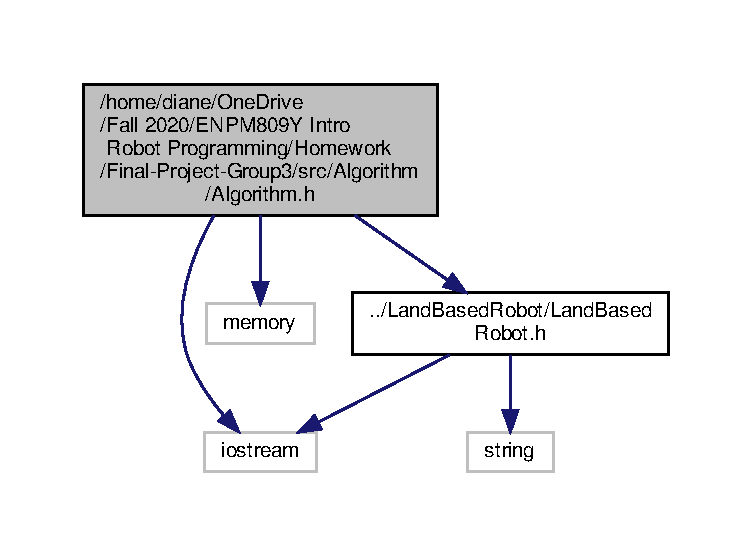
\includegraphics[width=350pt]{_algorithm_8h__incl}
\end{center}
\end{figure}
This graph shows which files directly or indirectly include this file\+:
\nopagebreak
\begin{figure}[H]
\begin{center}
\leavevmode
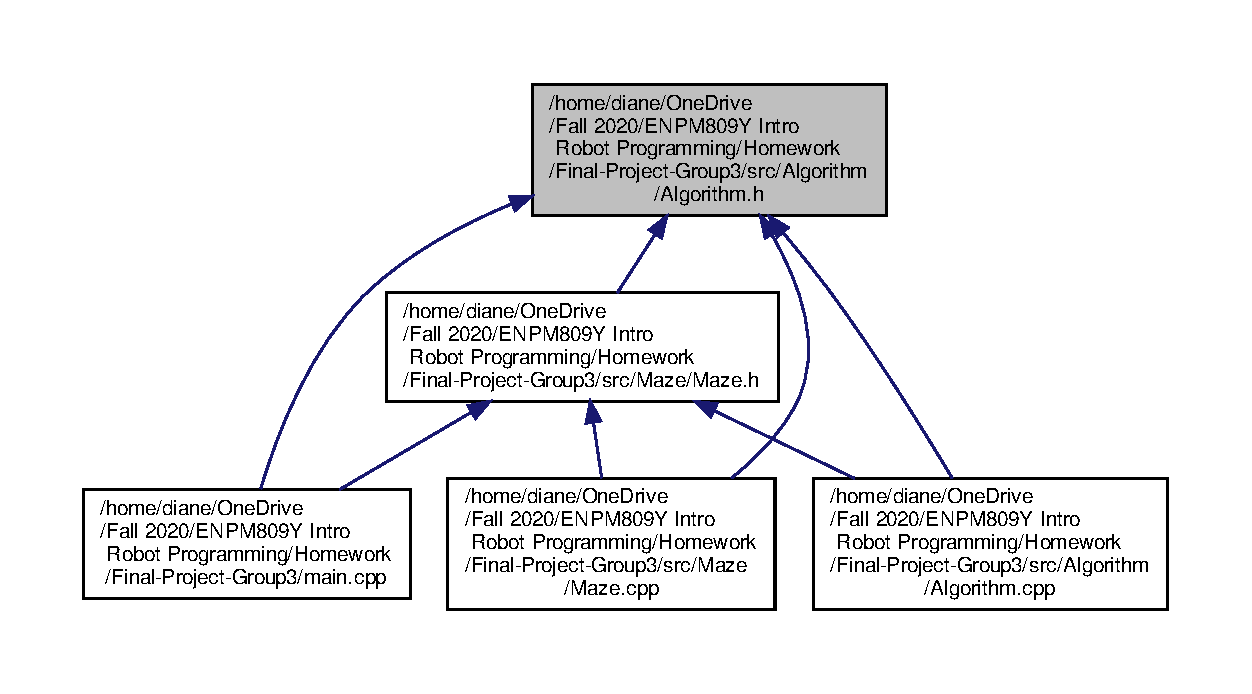
\includegraphics[width=350pt]{_algorithm_8h__dep__incl}
\end{center}
\end{figure}
\subsection*{Classes}
\begin{DoxyCompactItemize}
\item 
class \hyperlink{classfp_1_1_algorithm}{fp\+::\+Algorithm}
\item 
struct \hyperlink{structfp_1_1_algorithm_1_1_position}{fp\+::\+Algorithm\+::\+Position}
\end{DoxyCompactItemize}
\subsection*{Namespaces}
\begin{DoxyCompactItemize}
\item 
 \hyperlink{namespacefp}{fp}
\end{DoxyCompactItemize}

\hypertarget{api_8cpp}{}\section{/home/diane/\+One\+Drive/\+Fall 2020/\+E\+N\+P\+M809Y Intro Robot Programming/\+Homework/\+Final-\/\+Project-\/\+Group3/src/\+A\+P\+I/api.cpp File Reference}
\label{api_8cpp}\index{/home/diane/\+One\+Drive/\+Fall 2020/\+E\+N\+P\+M809\+Y Intro Robot Programming/\+Homework/\+Final-\/\+Project-\/\+Group3/src/\+A\+P\+I/api.\+cpp@{/home/diane/\+One\+Drive/\+Fall 2020/\+E\+N\+P\+M809\+Y Intro Robot Programming/\+Homework/\+Final-\/\+Project-\/\+Group3/src/\+A\+P\+I/api.\+cpp}}
{\ttfamily \#include \char`\"{}api.\+h\char`\"{}}\newline
{\ttfamily \#include $<$cstdlib$>$}\newline
{\ttfamily \#include $<$iostream$>$}\newline
Include dependency graph for api.\+cpp\+:\nopagebreak
\begin{figure}[H]
\begin{center}
\leavevmode
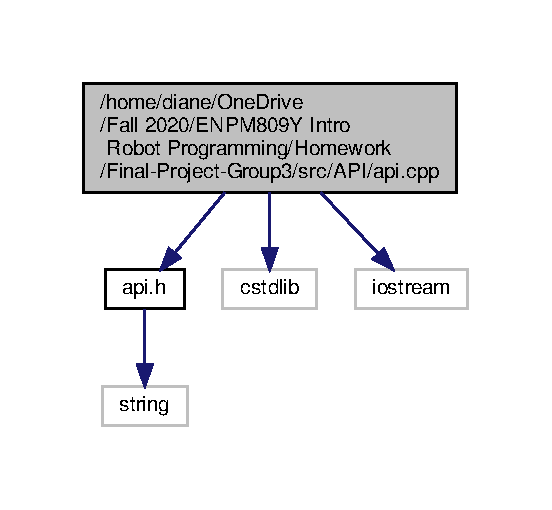
\includegraphics[width=265pt]{api_8cpp__incl}
\end{center}
\end{figure}

\hypertarget{api_8h}{}\section{/home/diane/\+One\+Drive/\+Fall 2020/\+E\+N\+P\+M809Y Intro Robot Programming/\+Homework/\+Final-\/\+Project-\/\+Group3/src/\+A\+P\+I/api.h File Reference}
\label{api_8h}\index{/home/diane/\+One\+Drive/\+Fall 2020/\+E\+N\+P\+M809\+Y Intro Robot Programming/\+Homework/\+Final-\/\+Project-\/\+Group3/src/\+A\+P\+I/api.\+h@{/home/diane/\+One\+Drive/\+Fall 2020/\+E\+N\+P\+M809\+Y Intro Robot Programming/\+Homework/\+Final-\/\+Project-\/\+Group3/src/\+A\+P\+I/api.\+h}}
{\ttfamily \#include $<$string$>$}\newline
Include dependency graph for api.\+h\+:\nopagebreak
\begin{figure}[H]
\begin{center}
\leavevmode
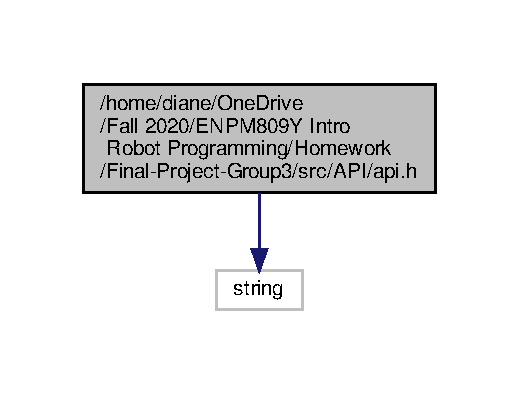
\includegraphics[width=249pt]{api_8h__incl}
\end{center}
\end{figure}
This graph shows which files directly or indirectly include this file\+:\nopagebreak
\begin{figure}[H]
\begin{center}
\leavevmode
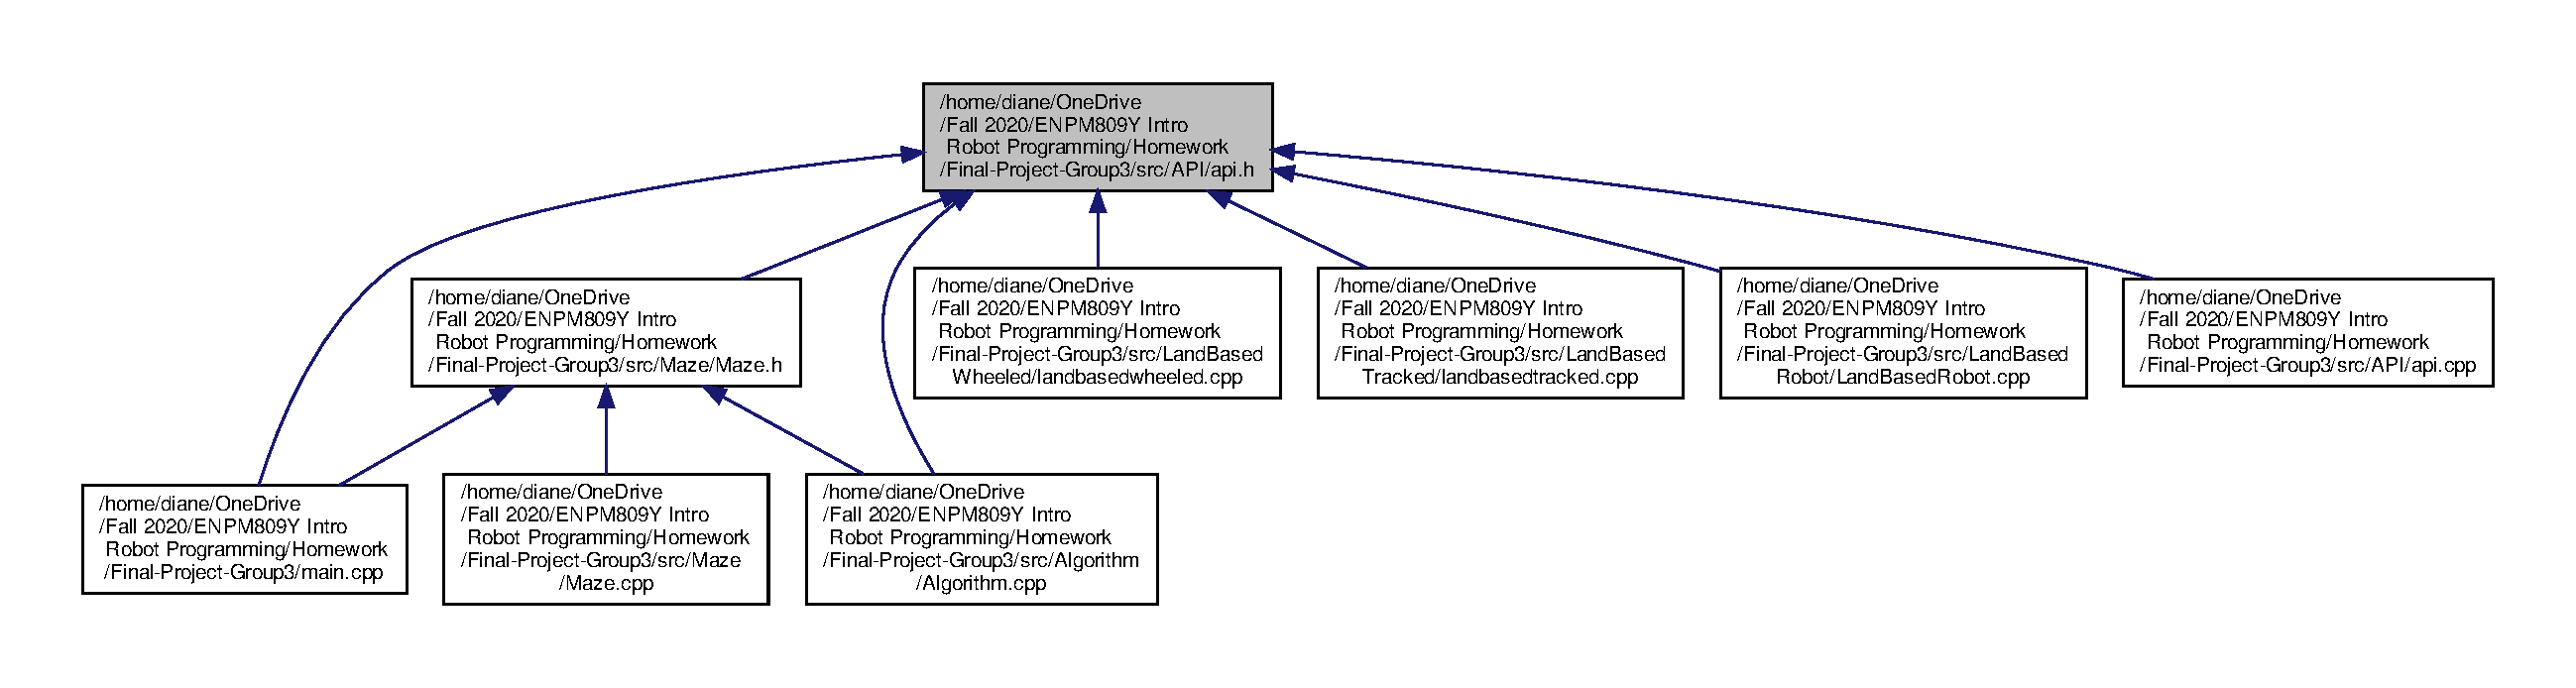
\includegraphics[width=350pt]{api_8h__dep__incl}
\end{center}
\end{figure}
\subsection*{Classes}
\begin{DoxyCompactItemize}
\item 
class \hyperlink{classfp_1_1_a_p_i}{fp\+::\+A\+PI}
\end{DoxyCompactItemize}
\subsection*{Namespaces}
\begin{DoxyCompactItemize}
\item 
 \hyperlink{namespacefp}{fp}
\end{DoxyCompactItemize}

\hypertarget{_land_based_robot_8cpp}{}\section{/home/diane/\+One\+Drive/\+Fall 2020/\+E\+N\+P\+M809Y Intro Robot Programming/\+Homework/\+R\+W\+A3-\/\+Group3/\+Land\+Based\+Robot/\+Land\+Based\+Robot.cpp File Reference}
\label{_land_based_robot_8cpp}\index{/home/diane/\+One\+Drive/\+Fall 2020/\+E\+N\+P\+M809\+Y Intro Robot Programming/\+Homework/\+R\+W\+A3-\/\+Group3/\+Land\+Based\+Robot/\+Land\+Based\+Robot.\+cpp@{/home/diane/\+One\+Drive/\+Fall 2020/\+E\+N\+P\+M809\+Y Intro Robot Programming/\+Homework/\+R\+W\+A3-\/\+Group3/\+Land\+Based\+Robot/\+Land\+Based\+Robot.\+cpp}}
{\ttfamily \#include \char`\"{}Land\+Based\+Robot.\+h\char`\"{}}\newline
{\ttfamily \#include $<$iostream$>$}\newline
Include dependency graph for Land\+Based\+Robot.\+cpp\+:\nopagebreak
\begin{figure}[H]
\begin{center}
\leavevmode
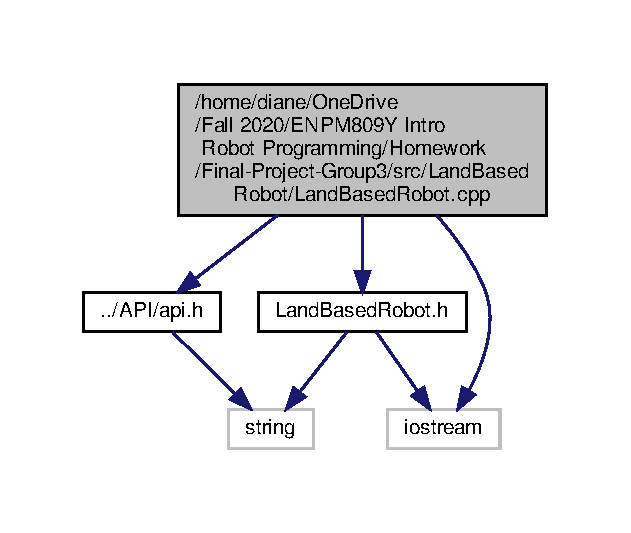
\includegraphics[width=275pt]{_land_based_robot_8cpp__incl}
\end{center}
\end{figure}
\subsection*{Namespaces}
\begin{DoxyCompactItemize}
\item 
 \hyperlink{namespacerwa3}{rwa3}
\end{DoxyCompactItemize}

\hypertarget{_land_based_robot_8h}{}\section{/home/diane/\+One\+Drive/\+Fall 2020/\+E\+N\+P\+M809Y Intro Robot Programming/\+Homework/\+R\+W\+A3-\/\+Group3/\+Land\+Based\+Robot/\+Land\+Based\+Robot.h File Reference}
\label{_land_based_robot_8h}\index{/home/diane/\+One\+Drive/\+Fall 2020/\+E\+N\+P\+M809\+Y Intro Robot Programming/\+Homework/\+R\+W\+A3-\/\+Group3/\+Land\+Based\+Robot/\+Land\+Based\+Robot.\+h@{/home/diane/\+One\+Drive/\+Fall 2020/\+E\+N\+P\+M809\+Y Intro Robot Programming/\+Homework/\+R\+W\+A3-\/\+Group3/\+Land\+Based\+Robot/\+Land\+Based\+Robot.\+h}}
{\ttfamily \#include $<$string$>$}\newline
{\ttfamily \#include $<$iostream$>$}\newline
{\ttfamily \#include $<$utility$>$}\newline
Include dependency graph for Land\+Based\+Robot.\+h\+:\nopagebreak
\begin{figure}[H]
\begin{center}
\leavevmode
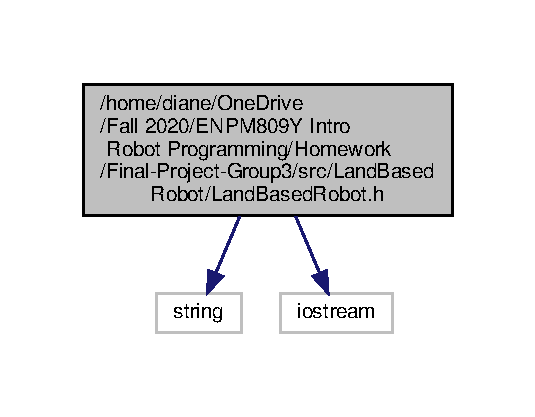
\includegraphics[width=252pt]{_land_based_robot_8h__incl}
\end{center}
\end{figure}
This graph shows which files directly or indirectly include this file\+:\nopagebreak
\begin{figure}[H]
\begin{center}
\leavevmode
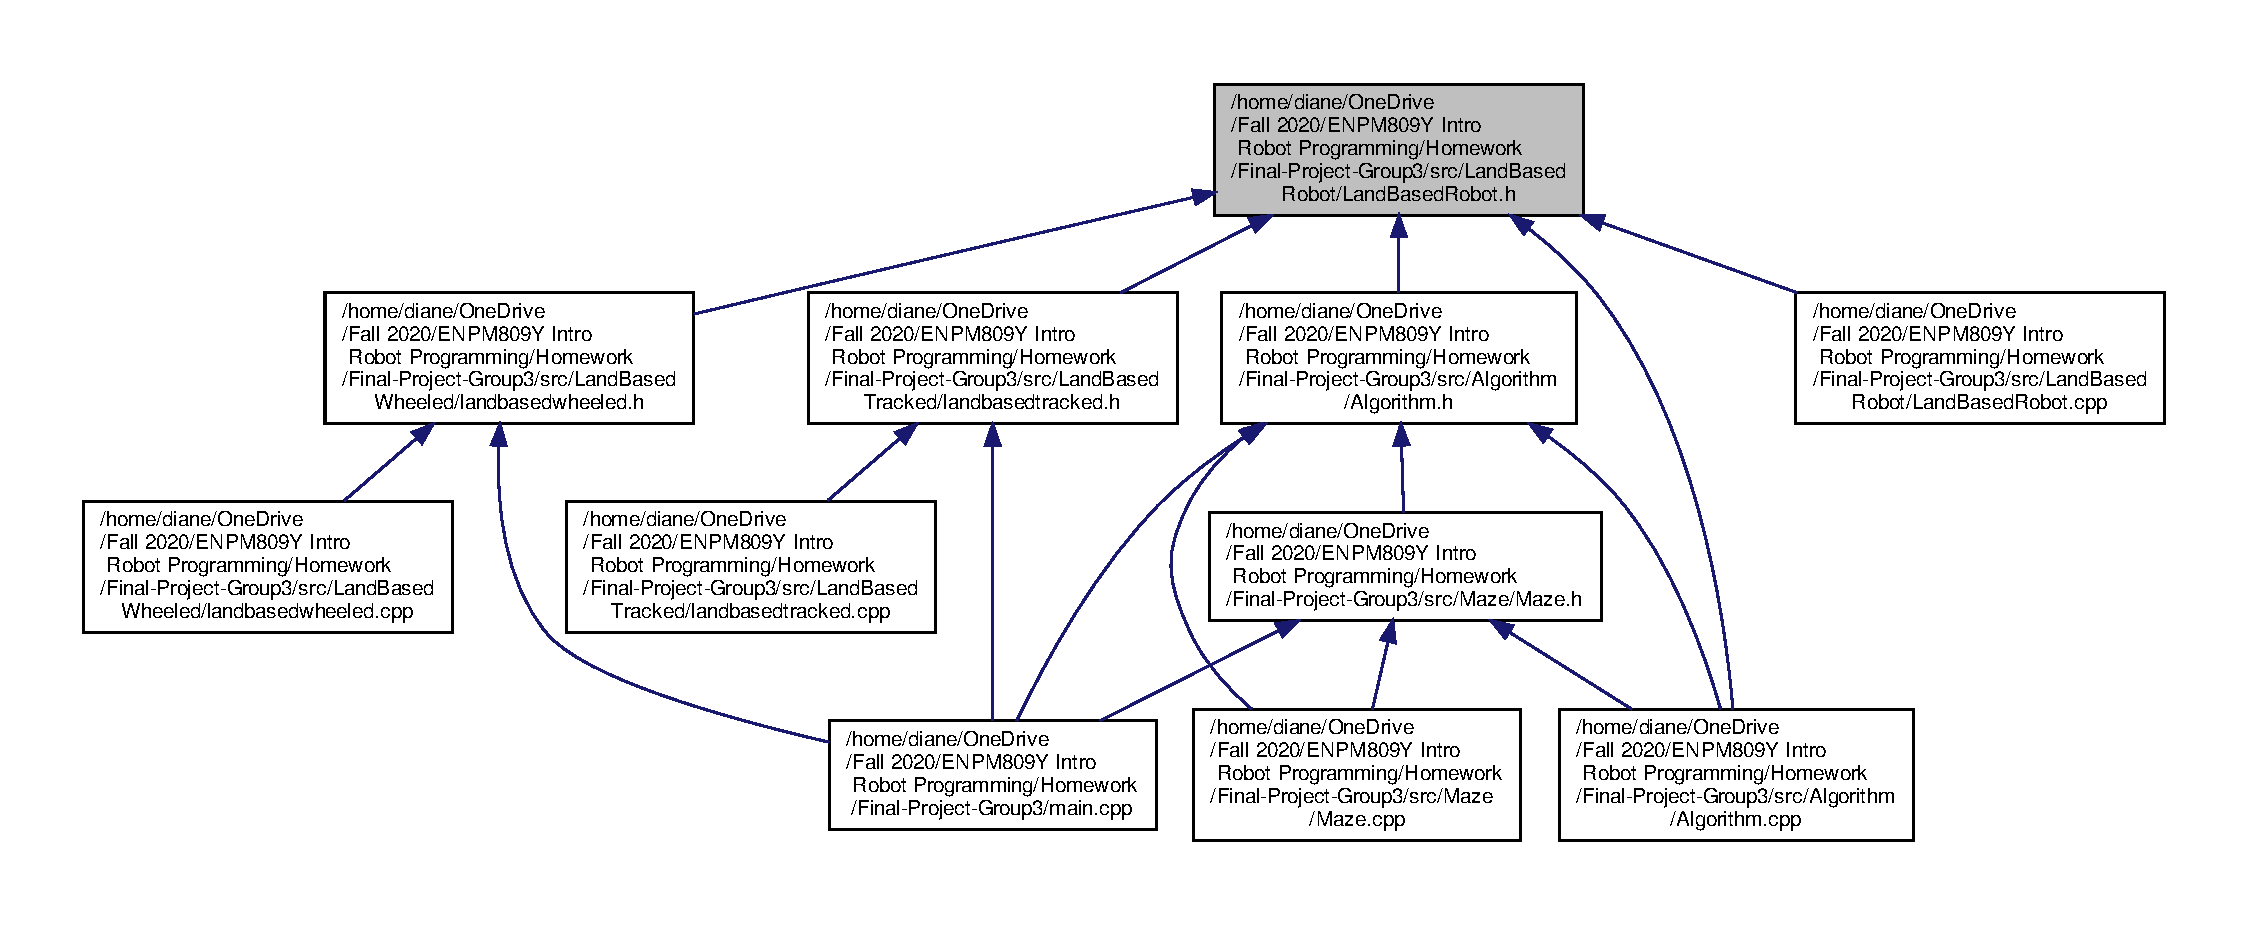
\includegraphics[width=350pt]{_land_based_robot_8h__dep__incl}
\end{center}
\end{figure}
\subsection*{Classes}
\begin{DoxyCompactItemize}
\item 
class \hyperlink{classrwa3_1_1_land_based_robot}{rwa3\+::\+Land\+Based\+Robot}
\end{DoxyCompactItemize}
\subsection*{Namespaces}
\begin{DoxyCompactItemize}
\item 
 \hyperlink{namespacerwa3}{rwa3}
\end{DoxyCompactItemize}

\hypertarget{landbasedtracked_8cpp}{}\section{/home/diane/\+One\+Drive/\+Fall 2020/\+E\+N\+P\+M809Y Intro Robot Programming/\+Homework/\+R\+W\+A3-\/\+Group3/\+Land\+Based\+Tracked/landbasedtracked.cpp File Reference}
\label{landbasedtracked_8cpp}\index{/home/diane/\+One\+Drive/\+Fall 2020/\+E\+N\+P\+M809\+Y Intro Robot Programming/\+Homework/\+R\+W\+A3-\/\+Group3/\+Land\+Based\+Tracked/landbasedtracked.\+cpp@{/home/diane/\+One\+Drive/\+Fall 2020/\+E\+N\+P\+M809\+Y Intro Robot Programming/\+Homework/\+R\+W\+A3-\/\+Group3/\+Land\+Based\+Tracked/landbasedtracked.\+cpp}}
{\ttfamily \#include \char`\"{}landbasedtracked.\+h\char`\"{}}\newline
{\ttfamily \#include $<$iostream$>$}\newline
Include dependency graph for landbasedtracked.\+cpp\+:\nopagebreak
\begin{figure}[H]
\begin{center}
\leavevmode
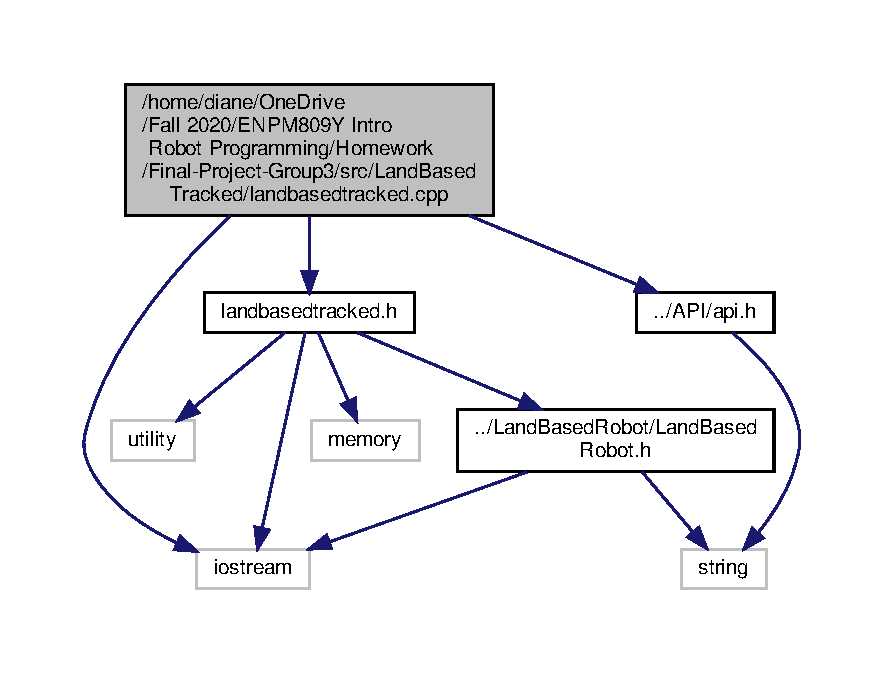
\includegraphics[width=350pt]{landbasedtracked_8cpp__incl}
\end{center}
\end{figure}

\hypertarget{landbasedtracked_8h}{}\section{/home/diane/\+One\+Drive/\+Fall 2020/\+E\+N\+P\+M809Y Intro Robot Programming/\+Homework/\+Final-\/\+Project-\/\+Group3/src/\+Land\+Based\+Tracked/landbasedtracked.h File Reference}
\label{landbasedtracked_8h}\index{/home/diane/\+One\+Drive/\+Fall 2020/\+E\+N\+P\+M809\+Y Intro Robot Programming/\+Homework/\+Final-\/\+Project-\/\+Group3/src/\+Land\+Based\+Tracked/landbasedtracked.\+h@{/home/diane/\+One\+Drive/\+Fall 2020/\+E\+N\+P\+M809\+Y Intro Robot Programming/\+Homework/\+Final-\/\+Project-\/\+Group3/src/\+Land\+Based\+Tracked/landbasedtracked.\+h}}
{\ttfamily \#include $<$iostream$>$}\newline
{\ttfamily \#include $<$memory$>$}\newline
{\ttfamily \#include $<$utility$>$}\newline
{\ttfamily \#include \char`\"{}../\+Land\+Based\+Robot/\+Land\+Based\+Robot.\+h\char`\"{}}\newline
Include dependency graph for landbasedtracked.\+h\+:\nopagebreak
\begin{figure}[H]
\begin{center}
\leavevmode
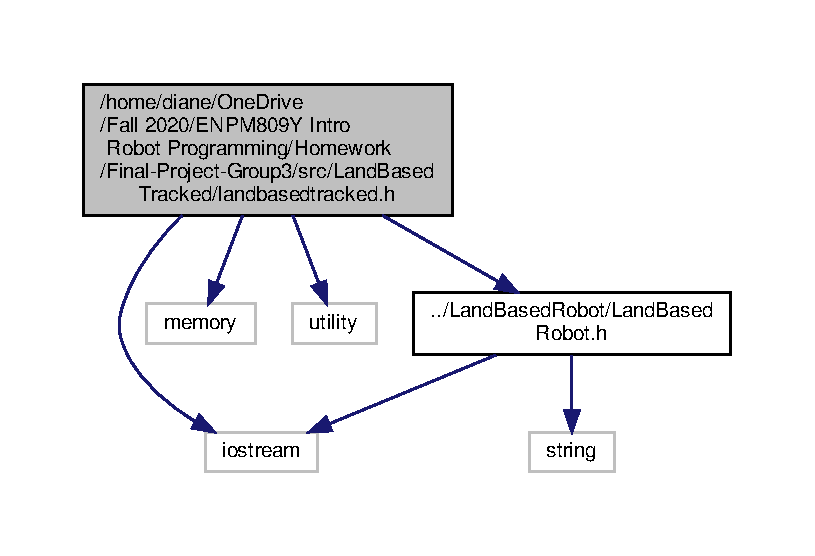
\includegraphics[width=350pt]{landbasedtracked_8h__incl}
\end{center}
\end{figure}
This graph shows which files directly or indirectly include this file\+:\nopagebreak
\begin{figure}[H]
\begin{center}
\leavevmode
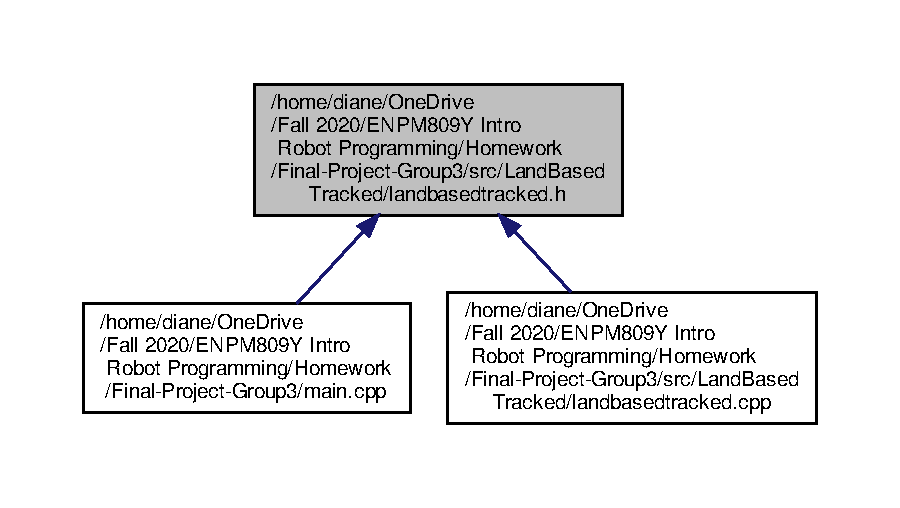
\includegraphics[width=350pt]{landbasedtracked_8h__dep__incl}
\end{center}
\end{figure}
\subsection*{Classes}
\begin{DoxyCompactItemize}
\item 
class \hyperlink{classfp_1_1_land_based_tracked}{fp\+::\+Land\+Based\+Tracked}
\end{DoxyCompactItemize}
\subsection*{Namespaces}
\begin{DoxyCompactItemize}
\item 
 \hyperlink{namespacefp}{fp}
\end{DoxyCompactItemize}

\hypertarget{landbasedwheeled_8cpp}{}\section{/home/diane/\+One\+Drive/\+Fall 2020/\+E\+N\+P\+M809Y Intro Robot Programming/\+Homework/\+R\+W\+A3-\/\+Group3/\+Land\+Based\+Wheeled/landbasedwheeled.cpp File Reference}
\label{landbasedwheeled_8cpp}\index{/home/diane/\+One\+Drive/\+Fall 2020/\+E\+N\+P\+M809\+Y Intro Robot Programming/\+Homework/\+R\+W\+A3-\/\+Group3/\+Land\+Based\+Wheeled/landbasedwheeled.\+cpp@{/home/diane/\+One\+Drive/\+Fall 2020/\+E\+N\+P\+M809\+Y Intro Robot Programming/\+Homework/\+R\+W\+A3-\/\+Group3/\+Land\+Based\+Wheeled/landbasedwheeled.\+cpp}}
{\ttfamily \#include \char`\"{}landbasedwheeled.\+h\char`\"{}}\newline
{\ttfamily \#include $<$iostream$>$}\newline
Include dependency graph for landbasedwheeled.\+cpp\+:\nopagebreak
\begin{figure}[H]
\begin{center}
\leavevmode
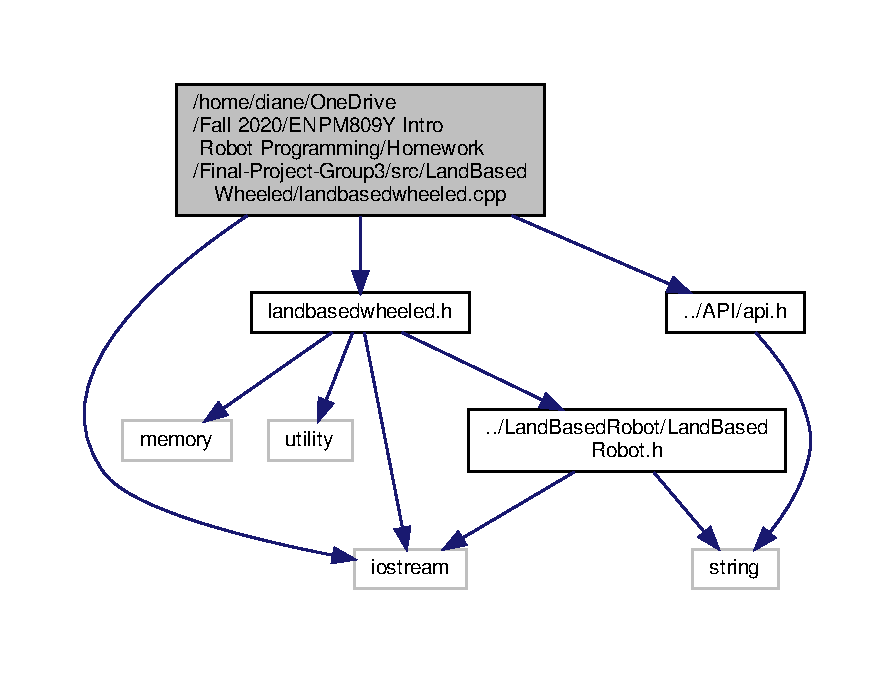
\includegraphics[width=350pt]{landbasedwheeled_8cpp__incl}
\end{center}
\end{figure}

\hypertarget{landbasedwheeled_8h}{}\section{/home/diane/\+One\+Drive/\+Fall 2020/\+E\+N\+P\+M809Y Intro Robot Programming/\+Homework/\+Final-\/\+Project-\/\+Group3/src/\+Land\+Based\+Wheeled/landbasedwheeled.h File Reference}
\label{landbasedwheeled_8h}\index{/home/diane/\+One\+Drive/\+Fall 2020/\+E\+N\+P\+M809\+Y Intro Robot Programming/\+Homework/\+Final-\/\+Project-\/\+Group3/src/\+Land\+Based\+Wheeled/landbasedwheeled.\+h@{/home/diane/\+One\+Drive/\+Fall 2020/\+E\+N\+P\+M809\+Y Intro Robot Programming/\+Homework/\+Final-\/\+Project-\/\+Group3/src/\+Land\+Based\+Wheeled/landbasedwheeled.\+h}}
{\ttfamily \#include \char`\"{}../\+Land\+Based\+Robot/\+Land\+Based\+Robot.\+h\char`\"{}}\newline
{\ttfamily \#include $<$iostream$>$}\newline
{\ttfamily \#include $<$memory$>$}\newline
{\ttfamily \#include $<$utility$>$}\newline
Include dependency graph for landbasedwheeled.\+h\+:\nopagebreak
\begin{figure}[H]
\begin{center}
\leavevmode
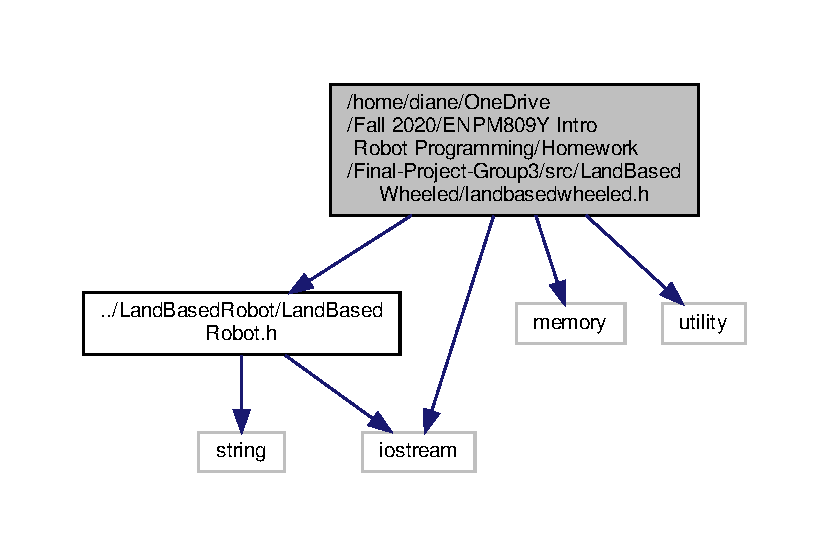
\includegraphics[width=350pt]{landbasedwheeled_8h__incl}
\end{center}
\end{figure}
This graph shows which files directly or indirectly include this file\+:\nopagebreak
\begin{figure}[H]
\begin{center}
\leavevmode
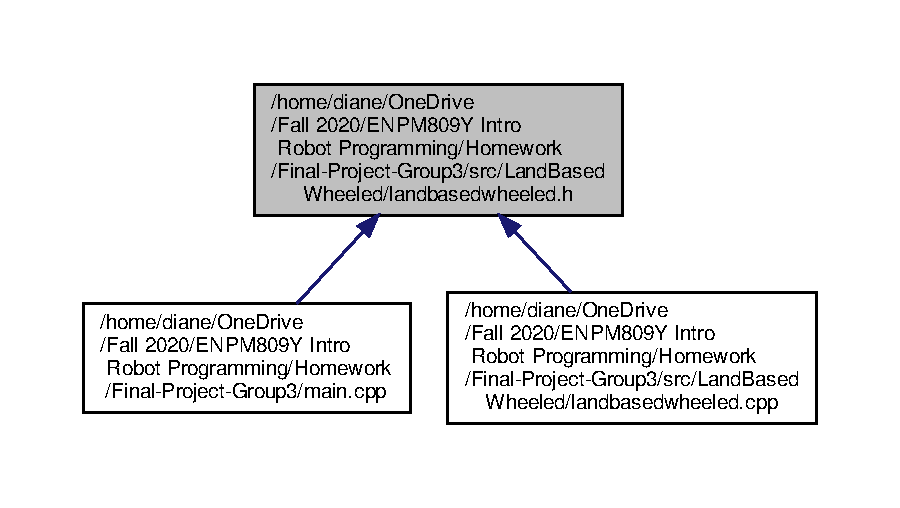
\includegraphics[width=350pt]{landbasedwheeled_8h__dep__incl}
\end{center}
\end{figure}
\subsection*{Classes}
\begin{DoxyCompactItemize}
\item 
class \hyperlink{classfp_1_1_land_based_wheeled}{fp\+::\+Land\+Based\+Wheeled}
\end{DoxyCompactItemize}
\subsection*{Namespaces}
\begin{DoxyCompactItemize}
\item 
 \hyperlink{namespacefp}{fp}
\end{DoxyCompactItemize}

\hypertarget{_maze_8cpp}{}\section{/home/diane/\+One\+Drive/\+Fall 2020/\+E\+N\+P\+M809Y Intro Robot Programming/\+Homework/\+Final-\/\+Project-\/\+Group3/src/\+Maze/\+Maze.cpp File Reference}
\label{_maze_8cpp}\index{/home/diane/\+One\+Drive/\+Fall 2020/\+E\+N\+P\+M809\+Y Intro Robot Programming/\+Homework/\+Final-\/\+Project-\/\+Group3/src/\+Maze/\+Maze.\+cpp@{/home/diane/\+One\+Drive/\+Fall 2020/\+E\+N\+P\+M809\+Y Intro Robot Programming/\+Homework/\+Final-\/\+Project-\/\+Group3/src/\+Maze/\+Maze.\+cpp}}
{\ttfamily \#include \char`\"{}Maze.\+h\char`\"{}}\newline
{\ttfamily \#include \char`\"{}../\+Algorithm/\+Algorithm.\+h\char`\"{}}\newline
Include dependency graph for Maze.\+cpp\+:
\nopagebreak
\begin{figure}[H]
\begin{center}
\leavevmode
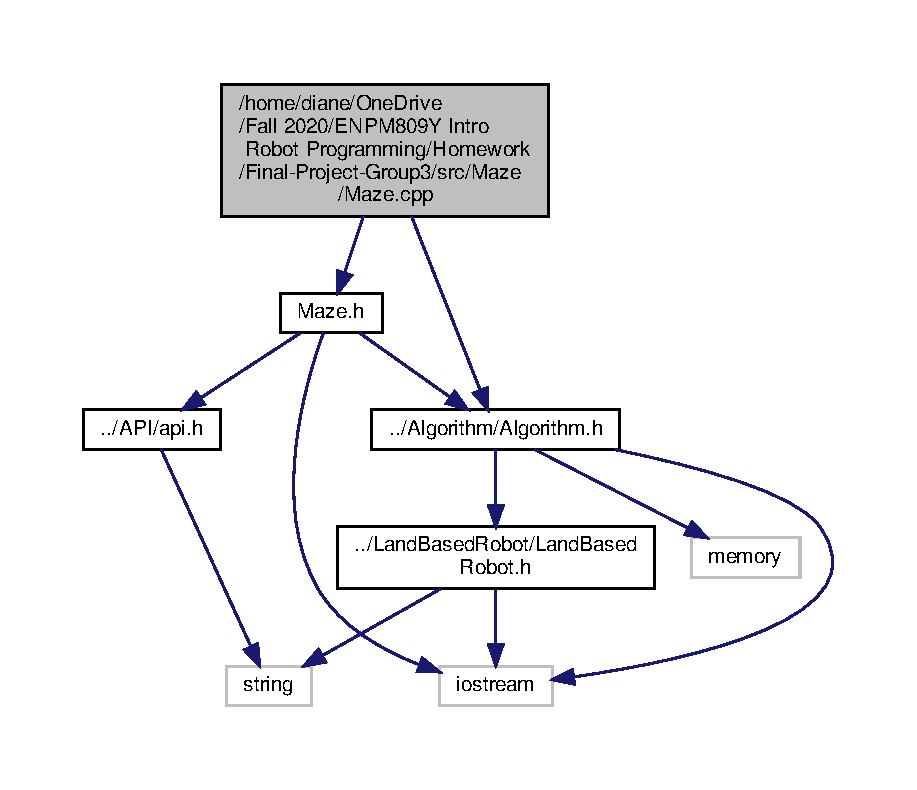
\includegraphics[width=350pt]{_maze_8cpp__incl}
\end{center}
\end{figure}
This graph shows which files directly or indirectly include this file\+:
\nopagebreak
\begin{figure}[H]
\begin{center}
\leavevmode
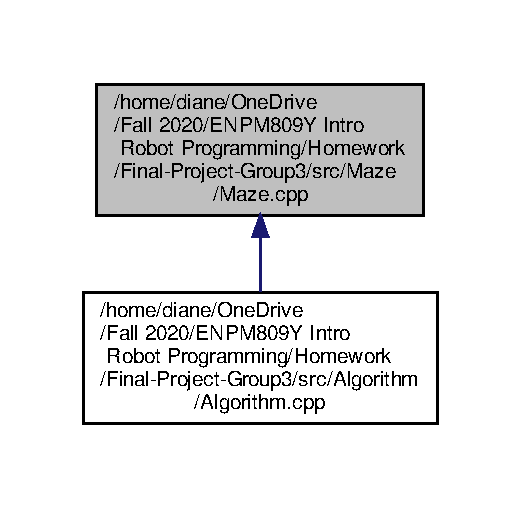
\includegraphics[width=250pt]{_maze_8cpp__dep__incl}
\end{center}
\end{figure}

\hypertarget{_maze_8h}{}\section{/home/diane/\+One\+Drive/\+Fall 2020/\+E\+N\+P\+M809Y Intro Robot Programming/\+Homework/\+Final-\/\+Project-\/\+Group3/src/\+Maze/\+Maze.h File Reference}
\label{_maze_8h}\index{/home/diane/\+One\+Drive/\+Fall 2020/\+E\+N\+P\+M809\+Y Intro Robot Programming/\+Homework/\+Final-\/\+Project-\/\+Group3/src/\+Maze/\+Maze.\+h@{/home/diane/\+One\+Drive/\+Fall 2020/\+E\+N\+P\+M809\+Y Intro Robot Programming/\+Homework/\+Final-\/\+Project-\/\+Group3/src/\+Maze/\+Maze.\+h}}
{\ttfamily \#include \char`\"{}../\+A\+P\+I/api.\+h\char`\"{}}\newline
{\ttfamily \#include \char`\"{}../\+Algorithm/\+Algorithm.\+h\char`\"{}}\newline
{\ttfamily \#include $<$iostream$>$}\newline
Include dependency graph for Maze.\+h\+:\nopagebreak
\begin{figure}[H]
\begin{center}
\leavevmode
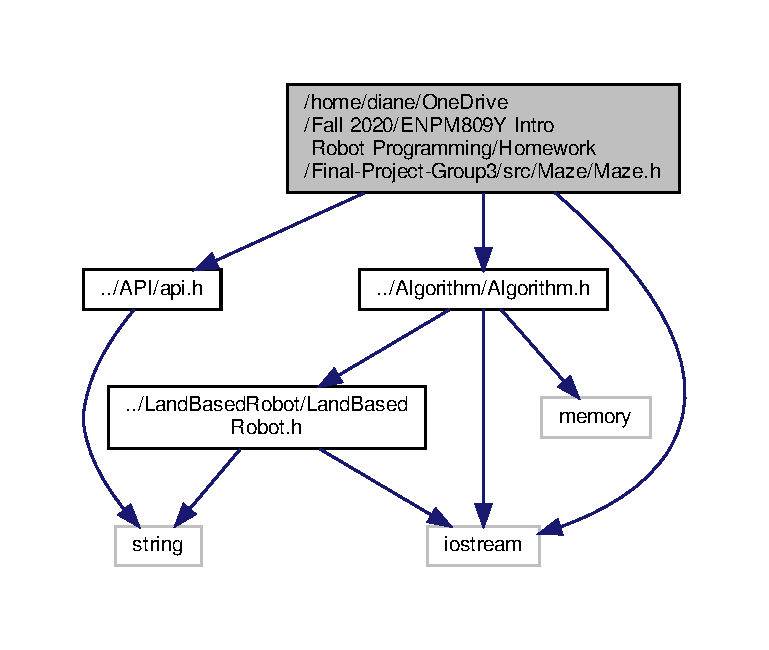
\includegraphics[width=350pt]{_maze_8h__incl}
\end{center}
\end{figure}
This graph shows which files directly or indirectly include this file\+:
\nopagebreak
\begin{figure}[H]
\begin{center}
\leavevmode
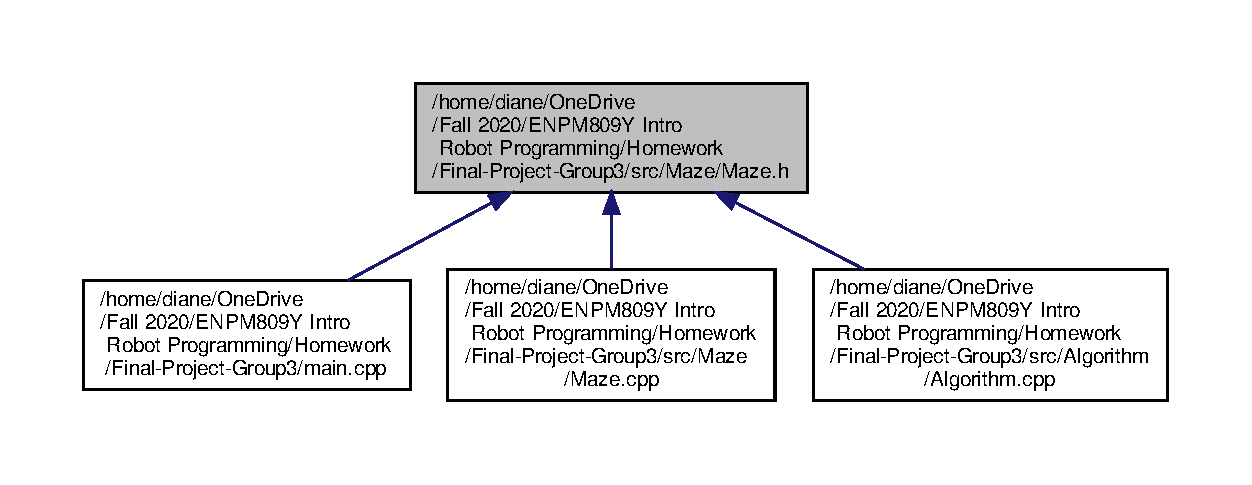
\includegraphics[width=350pt]{_maze_8h__dep__incl}
\end{center}
\end{figure}
\subsection*{Classes}
\begin{DoxyCompactItemize}
\item 
class \hyperlink{classfp_1_1_maze}{fp\+::\+Maze}
\end{DoxyCompactItemize}
\subsection*{Namespaces}
\begin{DoxyCompactItemize}
\item 
 \hyperlink{namespacefp}{fp}
\end{DoxyCompactItemize}

%--- End generated contents ---

% Index
\backmatter
\newpage
\phantomsection
\clearemptydoublepage
\addcontentsline{toc}{chapter}{Index}
\printindex

\end{document}
